% **************************************************
% Definicion del Documento
% **************************************************
\documentclass[paper=A4,twoside=true,openright,parskip=full,chapterprefix=true,11pt,headings=normal,bibliography=totoc,listof=totoc,titlepage=on,captions=tableabove,draft=false
]{scrreprt}

% **************************************************
% Configuracion
% **************************************************
% **************************************************
% Codificacion
% **************************************************
\PassOptionsToPackage{utf8}{inputenc}
\usepackage{inputenc}
\usepackage[nohints]{minitoc}
\usepackage{booktabs}
\usepackage{float}
\usepackage{caption}
\usepackage{array}
\usepackage{longtable}
\usepackage{pdfpages}
\usepackage{titlesec}
\usepackage[title,toc]{appendix}

% **************************************************
% Informacion y comandos para su reutilización
% **************************************************
\newcommand{\thesisTitle}{MODELO DE ARQUITECTURA EMPRESARIAL PARA LA EMPRESA MINSTITUTO.COM UTILIZANDO ARCHIMATE}
\newcommand{\thesisName}{José Daniel Peña}
\newcommand{\thesisCode}{20001020109}
\newcommand{\thesisSubject}{Trabajo de Grado}
\newcommand{\thesisDate}{febrero 20, 2016}
\newcommand{\thesisVersion}{1.0}

\newcommand{\thesisFirstReviewer}{Sandro Bolaños Castro}
\newcommand{\thesisFirstReviewerUniversity}{\protect{Universidad Distrital Francisco José de Caldas}}
\newcommand{\thesisFirstReviewerDepartment}{Ingenieria de Sistemas}

\newcommand{\thesisSecondReviewer}{Julio Barón Velandia}
\newcommand{\thesisSecondReviewerUniversity}{\protect{Universidad Distrital Francisco José de Caldas}}
\newcommand{\thesisSecondReviewerDepartment}{Ingenieria de Sistemas}

\newcommand{\thesisFirstSupervisor}{Jurado 1}
\newcommand{\thesisSecondSupervisor}{Jurado 2}

\newcommand{\thesisUniversity}{\protect{Universidad Distrital Francisco José de Caldas}}
\newcommand{\thesisUniversityDepartment}{Ingeniería de Sistemas}
\newcommand{\thesisUniversityInstitute}{Facultad de Ingeniería}
\newcommand{\thesisUniversityGroup}{}
\newcommand{\thesisUniversityCity}{Bogotá D.C.}
\newcommand{\thesisUniversityStreetAddress}{Cra. 8 \# 40-62}
\newcommand{\thesisUniversityPostalCode}{110231}

% **************************************************
% Configuracion de paquetes
% **************************************************
\usepackage[spanish]{babel}
\PassOptionsToPackage{
	figuresep=colon,
	sansserif=false,
	hangfigurecaption=false,
	hangsection=true,
	hangsubsection=true,
	colorize=full,
	colortheme=bluemagenta,
	bibsys=bibtex,
	bibfile=bib-refs,
	bibstyle=alphabetic,
	wrapfooter=false,
}{cleanthesis}
\usepackage{cleanthesis}

\hypersetup{
	pdftitle={\thesisTitle},
	pdfsubject={\thesisSubject},
	pdfauthor={\thesisName},
	plainpages=false,
	colorlinks=false,
	pdfborder={0 0 0},
	breaklinks=true,
	bookmarksnumbered=true,
	bookmarksopen=true
}
% **************************************************
% Comandos
% **************************************************
\renewcaptionname{spanish}{\figurename}{Fig.}
\renewcaptionname{spanish}{\tablename}{Tab.}
\mtcsetrules{*}{off}
\mtcsettitle{minitoc}{Contenido}
\graphicspath{{.}{imagenes/}}

% **************************************************
% Documento
% **************************************************
\begin{document}
	% --------------------------
	% Preliminares
	% --------------------------
	\pagenumbering{roman}
	\pagestyle{empty}
	% ------------------------------------  --> cover title page
\begin{titlepage}
	\pdfbookmark[0]{Portada}{Portada}
	\flushright
	\hfill
	\vfill
	{\LARGE\thesisTitle \par}
	\rule[5pt]{\textwidth}{.4pt} \par
	{\Large\thesisName}
	\vfill
	\textit{\large\thesisDate} \\
	Creatics
\end{titlepage}


% ------------------------------------  --> main title page
\begin{titlepage}
	\pdfbookmark[0]{Titulo}{Titulo}
	\tgherosfont
	\centering

	{\Large \thesisUniversity} \\[4mm]
	
\includegraphics{figuras/0} \\[2mm]
	\textsf{\thesisUniversityInstitute} \\
	\textsf{\thesisUniversityDepartment} \\
	\textsf{\thesisUniversityGroup} \\

	\vfill
	{\large \thesisSubject} \\[5mm]
	{\large \color{ctcolortitle}\textbf{\thesisTitle} \\[10mm]}
	{\Large \thesisName} \\
	{\Large \thesisCode} \\

	\vfill
	\begin{minipage}[t]{.27\textwidth}
		\raggedleft
		\textit{Director}
	\end{minipage}
	\hspace*{15pt}
	\begin{minipage}[t]{.65\textwidth}
		{\Large \thesisFirstReviewer} \\
		{\small \thesisFirstReviewerUniversity} \\[-1mm]
		{\small \thesisFirstReviewerDepartment}
	\end{minipage} \\[5mm]
	\begin{minipage}[t]{.27\textwidth}
		\raggedleft
		\textit{Revisor}
	\end{minipage}
	\hspace*{15pt}
	\begin{minipage}[t]{.65\textwidth}
		{\Large \thesisSecondReviewer} \\
		{\small \thesisSecondReviewerUniversity} \\[-1mm]
		{\small \thesisSecondReviewerDepartment}
	\end{minipage} \\[10mm]
	\begin{minipage}[t]{.27\textwidth}
		\raggedleft
		\textit{Jurados}
	\end{minipage}
	\hspace*{15pt}
	\begin{minipage}[t]{.65\textwidth}
		\thesisFirstSupervisor\ y \thesisSecondSupervisor
	\end{minipage} \\[10mm]
	
	\thesisDate \\

\end{titlepage}


% ------------------------------------  --> lower title back for single page layout
\hfill
\vfill
{
	\small
	\textbf{\thesisName} \\
	\textit{\thesisTitle} \\
	\thesisSubject, \thesisDate \\
	Director: \thesisFirstReviewer \\
	Revisor: \thesisSecondReviewer \\
	Jurados: \thesisFirstSupervisor\ y \thesisSecondSupervisor \\[1.5em]
	\textbf{\thesisUniversity} \\
	\textit{\thesisUniversityGroup} \\
	\thesisUniversityInstitute \\
	\thesisUniversityDepartment \\
	\thesisUniversityStreetAddress \\
	\thesisUniversityCity \\
	\thesisUniversityPostalCode
}
	\cleardoublepage
	\pagestyle{plain}
	\vspace*{\fill}
\begin{center}
	{\Large \textit{Dedicado a María P.}}\\[0.4cm]
\end{center}
\vspace*{\fill}
	\cleardoublepage
	\pdfbookmark[0]{Agradecimientos}{agradecimientos}
\vspace*{3cm}
\noindent\Huge\textsc{Agradecimientos}\\
\normalsize
\noindent\rule[2pt]{\textwidth}{0.8pt}
\hspace*{3cm}
	\cleardoublepage
	\pdfbookmark[0]{Resumen}{resumen}
\vspace*{3cm}
\noindent\Huge\textsc{Resumen}\\
\normalsize
\noindent\rule[2pt]{\textwidth}{0.8pt}
\hspace*{3cm}

El objetivo del trabajo de grado es el desarrollo de la arquitectura empresarial para la empresa Creatics y su producto Minstituto. La arquitectura empresarial se define como una metodología que a través de una visión integral de la organización realiza la alineación de la filosofía organizacional con los diferentes procesos al interior de la empresa, identificando la interrelaciones entre los mismos, teniendo en cuenta la estructura de ADM (Architecture Development Method), permitiendo que los procesos estratégicos y de apoyo tengan un horizonte definido formalmente.

Un instrumento fundamental para el desarrollo del trabajo de grado fue Archimate, que es un lenguaje gráfico por medio del cual se representa la arquitectura empresarial que soporta la operación de la empresa. Con esta herramienta se realizó la descripción de los diferentes puntos de vista que abarcan toda la operación generando la visión global de la misma y su respectiva alineación con los objetivos estratégicos.

{\large\textbf{Palabras Clave:}}
Archimate, Arquitectura, Patrones, Colosoft, Creatics

\newpage
\pdfbookmark[0]{Abstact}{Abstact}
\vspace*{3cm}
\noindent\Huge\textsc{Abstract}\\
\normalsize
\noindent\rule[2pt]{\textwidth}{0.8pt}
\hspace*{3cm}

The aim of this thesis is the development of enterprise architecture for the Creatics company and its product Minstituto. Enterprise Architecture is defined as a methodology in which through a holistic view of the organization the alignment of organizational philosophy with different processes within the company is performed, identifying the relationships between them, taking into account the ADM structure (Architecture Development Method), enabling that strategic and support processes have a formally defined horizon.

An essential tool for the development of the tesis was ArchiMate, which is a graphical language whereby enterprise architecture that supports the operation of the company is represented. With this tool the different views covering the entire operation were described, generating a global view of the organization and its alignment with the estrategic objectives.

	\cleardoublepage
	\dominitoc
	\setcounter{tocdepth}{2}
	\tableofcontents
	\cleardoublepage
	\listoffigures
	\cleardoublepage
	\listoftables
	% --------------------------
	% Cuerpo
	% --------------------------
	\cleardoublepage
	\pagenumbering{arabic}
	\setcounter{page}{1}
	\pagestyle{maincontentstyle}
	\cleardoublepage
	\vspace*{3cm}
\noindent\Huge\textsc{Introducción}\\
\normalsize
\noindent\rule[2pt]{\textwidth}{0.8pt}
\hspace*{3cm}

Con el trabajo desarrollado se elaboró una propuesta de Arquitectura empresarial para el producto mistituto.com de la empresa Creatics la cual se dedica al desarrollo de software.  Este proceso se generó a través de la identificación de las características organizacionales y la representación de sus componentes y sus relaciones de forma integral utilizando el lenguaje Archimate. \\ \\

La Arquitectura Empresarial es una metodología que describe formalmente el sistema visualizando de forma global los elementos de las organizaciones, su relación en la consecución de los objetivos estratégicos y su evolución en el tiempo.
Archimate es un lenguaje de modelamiento de Arquitectura empresarial que mediante un conjunto de símbolos y estructuras gráficas permite representar la arquitectura empresarial. \\ \\

El documento se encuentra dividido en cuatro partes; la primera parte contiene la contextualización, la cual incluye la descripción y filosofía organizacional de la empresa y la conceptualización.  En la segunda parte se desarrolla la arquitectura empresarial. En la tercera parte se presentan las conclusiones y por último la cuarta parte relaciona referencias bibliográficas.
	\part{Contextualización}
		\chapter{Descripción del proyecto}
\label{chap:Problema}
\textit{The first chapter introduces fluorescence-based DNA technology and highlights the motivation of the research conducted in the thesis}
\vfill
\minitoc
\newpage

\section{Definición del problema}
  \paragraph*{}
  Una de las mayores ventajas competitivas en una empresa es que la gestión de todos sus procesos y componentes estén alineados con su estrategia empresarial y su filosofía corporativa, sin embargo, realizar este proceso requiere una metodología que asegure que su planteamiento es efectivo. \\
  Creatics es una empresa en proceso de creación que requiere establecer estrategias de competitividad y sostenibilidad que la hagan desde el inicio una empresa sólida.

\section{Formulación del problema}
  \paragraph*{}
  ¿Es la Arquitectura Empresarial la metodología que permita alinear los procesos y componentes del producto mistituto.com de la empresa Creatics con el cumplimiento de sus objetivos estratégicos?

\section{Objetivos}
  \subsection{Objetivo General}
    \paragraph*{}
    Desarrollar una Arquitectura Empresarial para el producto mistituto.com de la empresa Creatics utilizando como herramienta el lenguaje de Arquitectura Archimate.

  \subsection{Objetivos Específicos}
    \begin{itemize}
      \item Identificar la filosofía y características organizacionales de Creatics.
      \item Establecer actores, roles y stakeholders dentro de los diferentes procesos.
      \item Determinar los procesos, datos, aplicaciones, infraestructura tecnológica y demás componentes para la modelación.
    \end{itemize}

\section{Alcance}
  \paragraph*{}
  Se desarrollará la Arquitectura Empresarial para el producto minstituto.com de la empresa Creatics utilizando el lenguaje de arquitectura Archimate.

\chapter{Presentación de la organización}
\label{chap:Descripcion}
\textit{The first chapter introduces fluorescence-based DNA technology and highlights the motivation of the research conducted in the thesis}
\vfill
\minitoc
\newpage

\section{Filosofía Organizacional}
  
  \subsection{Misión}
    \paragraph*{}
    Generamos soluciones tecnológicas que promueven el progreso de nuestros clientes contando con un equipo de trabajo altamente competitivo.
  
  \subsection{Visión}
    \paragraph*{}
    Ser reconocidos por nuestros productos innovadores principalmente en el sector de instituciones educativas.
  
  \subsection{Objetivos estratégicos}
    \begin{itemize}
  	  \item Proveer soluciones tecnológicas que permitan optimizar la gestión de la información en las instituciones educativas, generando renta para nuestros socios.
      \item Generar reconocimiento en el sector de instituciones educativas.
    \end{itemize}

  \subsection{Principios}
    \begin{itemize}
    	\item \textbf{Compromiso:} Orientamos nuestros esfuerzos al cumplimiento de las metas establecidas.
    	\item \textbf{Innovación:} Buscamos generar valor agregado a nuestros productos que permitan incrementar los beneficios a nuestros clientes.
    	\item \textbf{Enfoque al cliente:} Nuestros procesos se orientan en ofrecer el mejor servicio siendo respaldo para nuestros clientes.
    	\item \textbf{Confidencialidad:} Nuestros clientes cuentan con la garantía de que su información no será divulgada y tendrán un manejo apropiado de la información de su organización.
    	\item \textbf{Responsabilidad social y ambiental:} Buscamos beneficiar a nuestros colaboradores y a la sociedad al igual que el medio ambiente por medio de nuestros procesos internos.
    \end{itemize}
    
    \subsection{Valores}
      \begin{itemize}
		\item \textbf{Respeto:} Consiste en reconocer, aceptar y comprender los intereses y necesidades de todos los integrantes de la organización y de nuestros clientes.
		\item \textbf{Transparencia:} Generar procesos donde predomine la comunicación, la claridad y la honestidad.
		\item \textbf{Trabajo en equipo:} Buscamos integrar las habilidades y destrezas del equipo de profesionales en beneficio de nuestros clientes.
    \end{itemize}

\section{Estructura Organizacional}
  \begin{figure}[H]
  	\centering
  	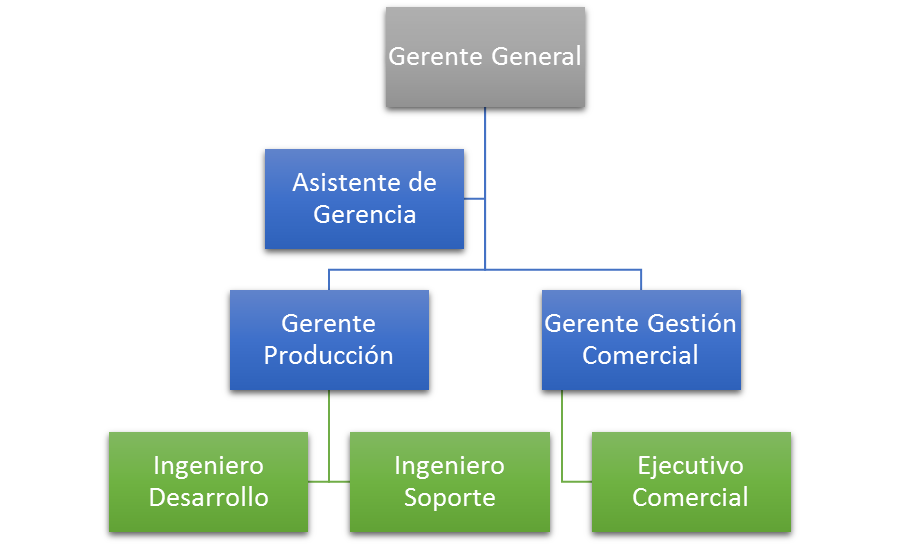
\includegraphics{figuras/1}
  	\captionsetup{width=.95\textwidth}
  	\caption{Organigrama Creatics}
  	\label{figura1}
  \end{figure}
  
\section{Mapa de Procesos}
  La organización con el fin de satisfacer las necesidades del cliente apoya su operación en tres procesos fundamentales: \\ \\
  \textbf{Estratégicos:} La gestión de dirección y la mejora continua dentro de su funcionamiento establecen las políticas y lineamientos que permiten llevar a cabo la misión. \\
  \textbf{Misionales:} Estos procesos llevan a cabo las operaciones orientadas a la satisfacción de las necesidades de los clientes. \\
  \textbf{Apoyo:} Son los procesos que brindan soporte a la gestión de los procesos estratégicos y misionales.

  \begin{figure}[H]
  	\centering
  	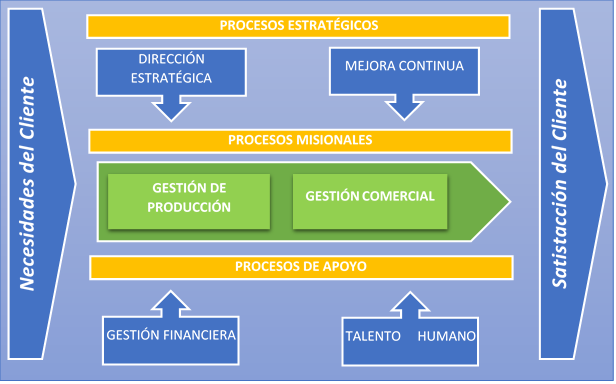
\includegraphics[scale=0.85]{figuras/2}
  	\captionsetup{width=.95\textwidth}
  	\caption{Mapa de Procesos}
  	\label{figura2}
  \end{figure}
		\chapter{Metodología y Cronograma de trabajo}
\label{chap:metodologia}
\textit{The first chapter introduces fluorescence-based DNA technology and highlights the motivation of the research conducted in the thesis}
\vfill
\minitoc
\newpage

\section{Metodología SCRUM}
\subsection{Visión General}
Scrum es un marco de trabajo en el que equipos cross-funcionales pueden crear productos o desarrollar proyectos de una forma iterativa e incremental. El desarrollo se estructura en ciclos de trabajo llamados Sprints (también conocidos como iteraciones). Estas iteraciones no deben durar más de cuatro semanas cada una (siendo dos semanas la duración más habitual) y tienen lugar una tras otra sin pausa entre ellas. Los Sprints están acotados en el tiempo – finalizan en una fecha determinada independientemente de si el trabajo ha finalizado por completo o no, y jamás se prorrogan. Normalmente los equipos Scrum escogen una duración de Sprint y la mantienen para todos sus Sprints hasta que mejoran y pueden emplear ciclos más cortos. Al principio de cada Sprint, un Equipo cross-funcional (de en torno a siete personas) selecciona elementos (peticiones del cliente) de una lista priorizada. El equipo acuerda un objetivo colectivo respecto a lo que creen que podrán entregar al final del Sprint, algo que sea tangible y que estará “terminado” por completo. Durante el Sprint no se podrán añadir nuevos elementos; Scrum se adapta a los cambios en el siguiente Sprint, pero el pequeño Sprint actual está pensado para concentrarnos en un objetivo pequeño, claro y relativamente estable. Todos los días el Equipo se reúne brevemente para inspeccionar su progreso y ajustar los siguientes pasos necesarios para completar el trabajo pendiente. Al final del Sprint, el Equipo revisa el Sprint con los diferentes Stakeholders (interesados e involucrados en el producto) y realiza una demostración de lo que han desarrollado. Se obtiene feedback que podrá ser incorporado en el siguiente Sprint. Scrum enfatiza un producto “funcionando” al final del Sprint que esté realmente “terminado”. En el caso del software, esto significa un sistema que está integrado, testado, con la documentación de usuario generada y potencialmente entregable.
  \begin{figure}[H]
  	\centering
  	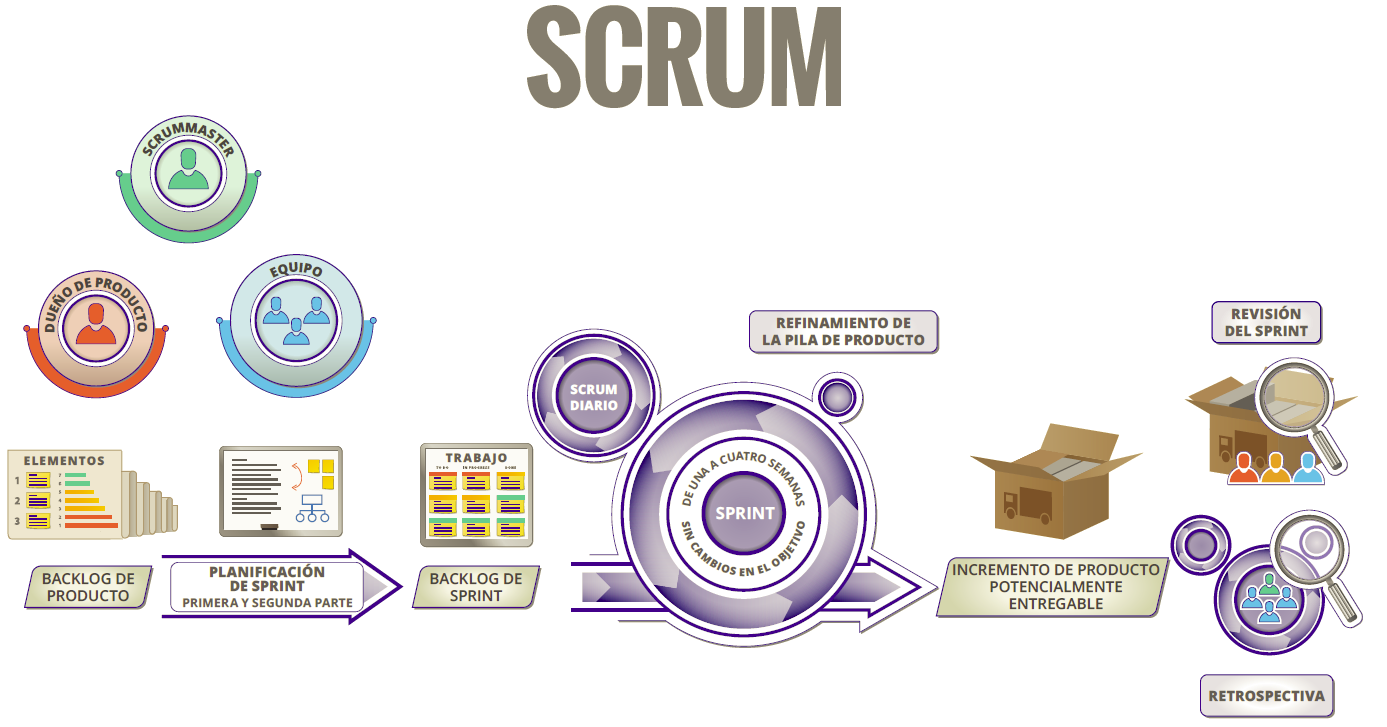
\includegraphics[scale=0.24]{figuras/2a}
  	\captionsetup{width=.95\textwidth}
  	\caption{Visión general de Scrum}
  	\label{figura2a}
  \end{figure}

\subsection{Teoría de Scrum}
Scrum se basa en la teoría de control de procesos empírica o empirismo. El empirismo asegura que el conocimiento procede de la experiencia y de tomar decisiones basándose en lo que se conoce, Scrum emplea un enfoque iterativo e incremental para optimizar la predictibilidad y el control del riesgo. \\

Tres pilares soportan toda la implementación del control de procesos empírico: transparencia, inspección y adaptación. \\
\begin{description}
	\item[Transparencia]  Los aspectos significativos del proceso deben ser visibles para aquellos que son responsables del resultado. La transparencia requiere que dichos aspectos sean definidos por un estándar común, de tal modo que los observadores compartan un entendimiento común de lo que se está viendo.
	\item[Inspección] Los usuarios de Scrum deben inspeccionar frecuentemente los artefactos de Scrum y el progreso hacia un objetivo, para detectar variaciones. Su inspección no debe ser tan frecuente como para que interfiera en el trabajo. Las inspecciones son más beneficiosas cuando se realizan de forma diligente por inspectores expertos, en el mismo lugar de trabajo.
	\item[Adaptación] Si un inspector determina que uno o más aspectos de un proceso se desvían de límites aceptables, y que el producto resultante no será aceptable, el proceso o el material que está siendo procesado deben ser ajustados. Dicho ajuste debe realizarse cuanto antes para minimizar desviaciones mayores.
\end{description}

Scrum prescribe cuatro eventos formales, contenidos dentro del Sprint, para la inspección y adaptación y son los siguientes.
  \begin{itemize}
  	\itemcolor{azull}
	\item Reunión de Planificación del Sprint (Sprint Planning Meeting)
	\item Scrum Diario (Daily Scrum)
	\item Revisión del Sprint (Sprint Review)
	\item Retrospectiva del Sprint (Sprint Retrospective)
  \end{itemize}
  
  \subsection{Eventos de Scrum}
  En Scrum existen eventos predefinidos con el fin de crear regularidad y minimizar la necesidad de reuniones no definidas en Scrum. Todos los eventos son bloques de tiempo (time-boxes), de tal modo que todos tienen una duración máxima. Una vez que comienza un Sprint, su duración es fija y no puede acortarse o alargarse. Los demás eventos pueden terminar siempre que se alcance el objetivo del evento, asegurando que se emplee una cantidad apropiada de tiempo sin permitir desperdicio en el proceso. \\
  
  Además del propio Sprint, que es un contenedor del resto de eventos, cada uno de los eventos de Scrum constituye una oportunidad formal para la inspección y adaptación de algún aspecto. Estos eventos están diseñados específicamente para habilitar las vitales transparencia e inspección. La falta de alguno de estos eventos da como resultado una reducción de la transparencia y constituye una oportunidad perdida para inspeccionar y adaptarse.
  
  \subsubsection{El Sprint}
  El corazón de Scrum es el Sprint, es un bloque de tiempo (time-box) de un mes o menos durante el cual se crea un incremento de producto “Terminado”, utilizable y potencialmente desplegable. Es más conveniente si la duración de los Sprints es consistente a lo largo del esfuerzo de desarrollo. Cada nuevo Sprint comienza inmediatamente después de la finalización del Sprint previo.
  
  \subsubsection{Revisión de Sprint}
  Al final del Sprint se lleva a cabo una Revisión de Sprint para inspeccionar el Incremento y adaptar la Lista de Producto si fuese necesario. Durante la Revisión de Sprint, el Equipo Scrum y los interesados colaboran acerca de lo que se hizo durante el Sprint. Basándose en esto, y en cualquier cambio a la Lista de Producto durante el Sprint.
  
  \subsubsection{Retrospectiva de Sprint}
  La Retrospectiva de Sprint es una oportunidad para el Equipo Scrum de inspeccionarse a sí mismo y crear un plan de mejoras que sean abordadas durante el siguiente Sprint. La Retrospectiva de Sprint tiene lugar después de la Revisión de Sprint y antes de la siguiente Reunión de Planificación de Sprint. Se trata de una reunión restringida a un bloque de tiempo de tres horas para Sprints de un mes.
  
  \subsection{El equipo Scrum}
  El Equipo Scrum consiste en un Dueño de Producto (Product Owner), el Equipo de Desarrollo (Development Team) y un Scrum Master. Los Equipos Scrum son autoorganizados y multifuncionales. El modelo de equipo en Scrum está diseñado para optimizar la flexibilidad, la creatividad y la productividad. \\
  
  Los Equipos Scrum entregan productos de forma iterativa e incremental, maximizando las oportunidades de obtener retroalimentación. Las entregas incrementales de producto terminado aseguran que siempre estará disponible una versión potencialmente útil y funcional del producto. 
  
  \subsubsection{El Dueño de Producto}
  El Dueño de Producto es el responsable de maximizar el valor del producto y del trabajo del Equipo de Desarrollo. El cómo se lleva a cabo esto podría variar ampliamente entre distintas organizaciones, Equipos Scrum e individuos.
  
  \subsubsection{El Equipo de Desarrollo}
  El Equipo de Desarrollo consiste en los profesionales que desempeñan el trabajo de entregar un Incremento de producto terminado, que potencialmente se pueda poner en producción, al final de cada Sprint. Solo los miembros del Equipo de Desarrollo participan en la creación del Incremento. Los Equipos de Desarrollo son estructurados y empoderados por la organización para organizar y gestionar su propio trabajo. La sinergia resultante optimiza la eficiencia y efectividad del Equipo de Desarrollo.
  
  \subsubsection{El Scrum Master}
  El Scrum Master es el responsable de asegurar que Scrum es entendido y adoptado. Los Scrum Masters hacen esto asegurándose de que el Equipo Scrum trabaja ajustándose a la teoría, prácticas y reglas de Scrum. El Scrum Master es un líder que está al servicio del Equipo Scrum. El Scrum Master ayuda a las personas externas al Equipo Scrum a entender qué interacciones con el Equipo Scrum pueden ser de ayuda y cuáles no. El Scrum Master ayuda a todos a modificar estas interacciones para maximizar el valor creado por el Equipo Scrum.

\section{Cronograma}
  \begin{figure}[H]
  	\centering
  	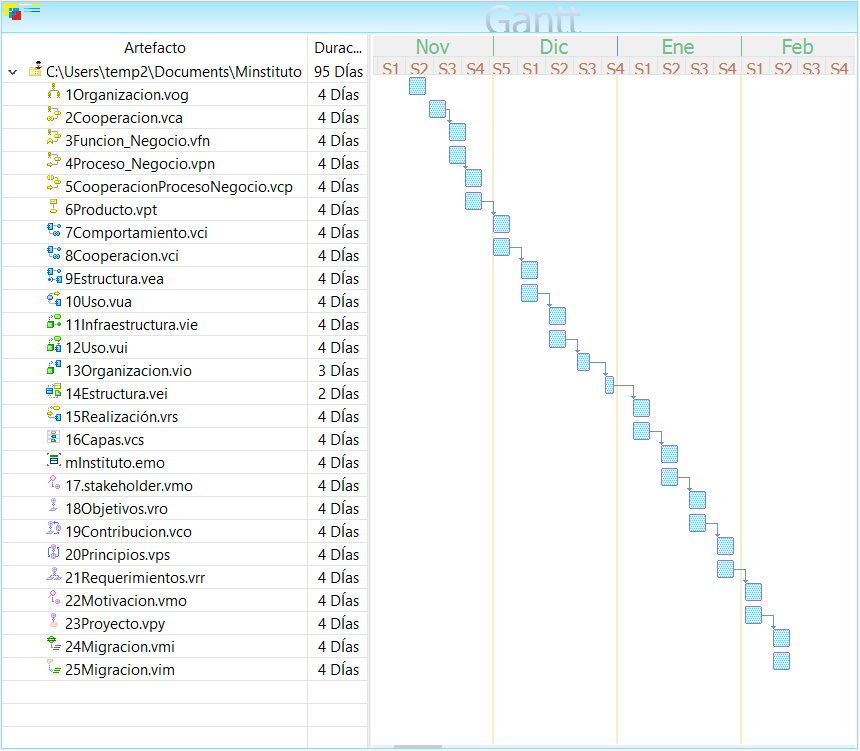
\includegraphics[scale=0.8]{figuras/3}
  	\captionsetup{width=.95\textwidth}
  	\caption{Cronograma}
  	\label{figura3}
  \end{figure}

\chapter{Arquitectura Empresarial}
\label{chap:aEmpresarial}
\textit{The first chapter introduces fluorescence-based DNA technology and highlights the motivation of the research conducted in the thesis}
\vfill
\minitoc
\newpage

\section{Arquitectura empresarial}
La definición de arquitectura empresarial surge frente a la necesidad de alinear las tecnologías de información a los objetivos estratégicos del negocio. Algunas definiciones de arquitectura empresarial se presentan a continuación:
  
  \begin{itemize}
  	\itemcolor{azull}
	\item \textit{IEEE Std. 1471-2000:} \\
	“…organización fundamental de un sistema, compuesta por sus componentes, las relaciones entre ellos y su ambiente y los principios que gobiernan su diseño y evolución”.
	\item \textit{The Open Group Architecture Framework:} \\
	“… la arquitectura empresarial se puede definir de dos posibles formas dependiendo del contexto en que se utilice 1) una descripción formal de un sistema o un plan detallado de un sistema a nivel de sus componentes para guiar su implementación; o 2) una estructura de componentes, sus interrelaciones, y los principios y guías que gobiernan su diseño y evolución en el tiempo”.
	\item \textit{International Enterprise Architecture Institute:} \\
	“El análisis y documentación de una organización en su estado actual y futuro desde las perspectivas de negocio, tecnología y estrategias integradas”.
	\item \textit{Federal Enterprise Architecture Framework, 1ra versión – 1999:}
	“… las arquitecturas empresariales son modelos que se aplican de manera sistemática y completa para definir el ámbito presente o futuro de una organización. Arquitecturas empresariales son esenciales para la evolución y desarrollo de nuevos sistemas de información que optimicen el valor de la misión de una organización…”
	\item \textit{Gartner Research:} \\
	“Una arquitectura empresarial es un proceso de planeamiento estratégico que traduce la visión y estrategias de negocio de una organización en un efectivo plan de cambio empresarial”.
  \end{itemize}

  En conclusión arquitectura empresarial es alinear los objetivos estratégicos de una organización con tecnología, describiendo el estado actual de la organización y proyectándonos a una visión futura con la implementación de nuevas tecnologías.
  
\section{Componentes de una Arquitectura Empresarial}
Los diferentes framework de arquitectura empresarial realizan un planteamiento de los componentes o dominios de arquitectura que son los elementos que definen el funcionamiento de una empresa. En la figura 1.5 se presentan los componentes de arquitectura empresarial: Arquitectura de negocio, arquitectura de información, arquitectura de sistemas de información y arquitectura tecnológica.
  
  \begin{figure}[H]
  	\centering
  	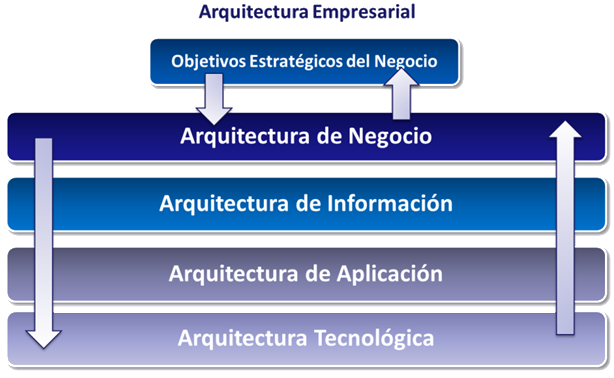
\includegraphics[scale=0.5]{figuras/4}
   	\captionsetup{width=.95\textwidth}
   	\caption{Componentes de Arquitectura Empresarial}
   	\label{figura4}
  \end{figure}
  
  \subsection{Arquitectura de negocio}
  Para Ralph Whittle, “La primera vista representa la arquitectura de negocio, la cual se encarga de la descripción de la estructura organizacional, de los procesos de negocio, los sistemas de planeación y control, los mecanismos de gobierno y administración de políticas y procedimientos en el entorno empresarial. Esta vista de arquitectura es la que refleja el valor del negocio obtenido de las sinergias y resultados que se producen desde las otras vistas de arquitectura que le preceden. La arquitectura de negocio recibe como insumo principal el plan estratégico de la empresa, los lineamientos corporativos, los indicadores de gestión, y se nutre de la misión, la visión, las estrategias y los objetivos corporativos. Las estrategias y objetivos de alto nivel los traducen en requerimientos que son relevantes para el negocio”.
  \subsection{Arquitectura de información}
  Para Richard Wurman, “La segunda vista representa la arquitectura de información, la cual describe los activos lógicos y físicos de los datos como un activo de la empresa, y la administración de los recursos de información; esta perspectiva muestra cómo los recursos de información están siendo administrados, compartidos y utilizados por la organización. \\
  La arquitectura de información es una disciplina que organiza conjuntos de información, permitiendo que cualquier persona los entienda y los integre a su propio conocimiento de manera simple. La construcción de una arquitectura de información requiere el levantamiento de un inventario de los objetos de negocio que representan los activos de información que están disponibles y que son utilizados por la organización. La información juega un rol fundamental para el funcionamiento de los sistemas de información y de los proceso de negocio”
  \subsection{Arquitectura de sistemas de información o aplicaciones}
  Para Richard Wurman, “La tercera vista representa la Arquitectura de sistemas de información que incorpora soluciones aplicativas que apoyan al negocio basadas en las capacidades funcionales requeridas y las estrategias de tecnología definidas, e identifica componentes y servicios que den respuesta a necesidades comunes de las áreas de negocio. La arquitectura aplicativa define qué clase de aplicaciones son relevantes para la empresa y lo que estas aplicaciones necesitan para gestionar los datos y presentar la información”.
  \subsection{Arquitectura tecnológica}
  Según Jaap Schekkerman, “La arquitectura técnica define la estrategia y arquitectura tecnológica en la infraestructura de TI, y el marco tecnológico de las plataformas computacionales y bases de datos que deben soportar las distintas soluciones del negocio, así como los mecanismos de almacenamiento de los datos e información, las redes de datos, los centros de procesamiento de datos y los servicios integrados de tecnología”.
 
\chapter{Framework y Modelado}
\label{chap:Archimate}
\textit{The first chapter introduces fluorescence-based DNA technology and highlights the motivation of the research conducted in the thesis}
\vfill
\minitoc
\newpage

\section{The Open Group}
The Open Group es un consorcio de la industria del software que provee estándares abiertos neutrales para la infraestructura de la informática. Fue formado a partir de la fusión de X/Open con OSF en 1996. The Open Group es muy famoso por sus sistemas de certificación de la marca UNIX; en el pasado el grupo fue reconocido por publicar el artículo Single UNIX Specification, el cual extiende los estándares de POSIX y es la definición oficial del sistema operativo conocido como UNIX. Sus miembros incluyen un conjunto de empresas y agencias gubernamentales, como por ejemplo Capgemini, Fujitsu, Hitachi, HP, IBM, NEC, Departamento de Defensa de Estados Unidos, NASA y otros.

\section{TOGAF}
TOGAF es un marco de referencia de arquitectura. En términos simples, TOGAF es una herramienta para asistir en la aceptación, creación, uso, y mantenimiento de arquitecturas. Está basado en un modelo iterativo de procesos apoyado por las mejores prácticas y un conjunto reutilizable de activos arquitectónicos existentes. \\

TOGAF es desarrollado y mantenido por el Foro de Arquitectura de The Open Group. La primera versión de TOGAF, desarrollada en 1995, se basó en el Marco de Referencia de Arquitectura Técnica para la Gestión de la Información del Ministerio de Defensa Estadounidense (TAFIM por sus siglas en inglés). Comenzando con esta solida fundación, el Foro de Arquitectura de The Open Group ha desarrollado versiones sucesivas de TOGAF con regularidad y ha publicado cada una en el sitio web público de The Open Group. \\

Según The Open Group, el 80\% de las grandes organizaciones a nivel mundial ha adoptado TOGAF como marco de referencia para sus Arquitecturas Empresariales; así mismo, decenas de miles de personas en todo el mundo han recibido formación y certificación en el marco del programa 'Open CA'.

Por otro lado, TOGAF se basa en modelos descriptivos que permiten definir la arquitectura desde diversos y estratégicos puntos de vista, para establecer a nivel general las necesidades, limitaciones y oportunidades del negocio.

  \subsection{¿Qué es Arquitectura para TOGAF?}
  Uno de los conceptos clave para cualquier proceso de arquitectura empresarial es la comprensión misma de la Arquitectura, ya que ésta determina, en parte, el enfoque desde el cual se adoptará el modelo. En TOGAF, “Arquitectura” tiene dos significados según el contexto:
  \begin{enumerate}
  	\itemcolor{azull}
  	\item Una descripción formal de un sistema o un plano detallado del sistema al nivel de sus componentes para orientar su implementación.
  	\item La estructura de componentes, sus interrelaciones y los principios y guías que gobiernan su diseño y evolución a través del tiempo.
  \end{enumerate}
  
  \subsection{Arquitectura soportada por TOGAF}
  TOGAF cubre el desarrollo de cuatro tipos relacionados en la arquitectura. Estos cuatro tipos de arquitectura son comúnmente aceptados como subconjuntos de una arquitectura empresarial, los cuales TOGAF esta diseñado para soportar.
  
    \begin{table}[H]
    	\centering
    	\begin{tabular}{p{5cm}p{8cm}}
    		\hline
    		\rowcolor[HTML]{0073a1}
    		{\color[HTML]{FFFFFF} \textbf{Tipo de Arquitectura}} & {\color[HTML]{FFFFFF} \textbf{Descripción}} \\
    		\hline
    		\textbf{Arquitectura de Negocio} & La estrategia de negocio, gobierno, organización y procesos clave de la organización. \\
    		\textbf{Arquitectura de datos} & La estructura de datos lógicos y fisicos que posee una organización y sus recursos de gestión de datos. \\
    		\textbf{Arquitectura de aplicación} & Un plano (blueprint en inglés) de las aplicaciones individuales a implementar, sus interacciones y sus relaciones con los procesos de negocio principales de la organización.
    		 \\
    		\textbf{Arquitectura tecnológica} & Las capacidades de software y hardware que se requieren para apoyar la implementación de servicios de negocio, datos y aplicación. Esto incluye infraestructura de IT, capa de mediación (middleware en ingles), redes, comunicaciones, procesamiento y estándares.
    		\\
    		\bottomrule
    	\end{tabular}
    	\captionsetup{width=.95\textwidth}
    	\caption{Tipos de la arquitectura soportados por TOGAF}
    	\label{tabla1} 
    \end{table}
    
  \subsection{Método de desarrollo de la Arquitectura (ADM)}
  El \textbf{ADM} describe cómo obtener una Arquitectura Empresarial que sea especifica para la organización y para responder a los requerimientos del negocio. El ADM es el componente principal de TOGAF y proporciona dirección a los arquitectos en varios niveles:
  \begin{itemize}
  	\itemcolor{azull}
  	\item Proporciona varias fases de desarrollo de arquitectura (Arquitectura de Negocio, Arquitecturas de Sistemas de Información, Arquitectura Tecnológica) en un ciclo, que sirve como una plantilla general de procesos para la actividad de desarrollo de la arquitectura.
  	\item Proporciona una narrativa de cada fase de la arquitectura, describiendo la fase en términos de objetivos, enfoque, entradas, pasos a seguir, y salidas. Las secciones de entradas y salidas proporcionan una definición de la estructura del contenido de arquitectura y entregables (una descripción detallada de las entradas de la fase y las salidas de la fase se da en el Marco de Referencia del Contenido Arquitectónico).
  	\item Proporciona resúmenes multi-fase que abordan también la Gestión de Requerimientos.
  \end{itemize}
  
  El ADM es el resultado de las contribuciones de numerosos profesionales de la arquitectura y constituye el núcleo de TOGAF. Es un método para obtener Arquitecturas Empresariales que son específicas para la organización, y está especialmente diseñado para responder a los requerimientos del negocio. El ADM describe:
  
  \begin{itemize}
  	\itemcolor{azull}
  	\item Un modo confiable y probado para desarrollar y utilizar una Arquitectura Empresarial
  	\item Un método para desarrollar arquitecturas en diferentes niveles1 (negocio, aplicaciones, datos, tecnología) que permiten al arquitecto asegurar que un conjunto complejo de requerimientos se aborden adecuadamente
  	\item Un conjunto de guías y técnicas para el desarrollo de arquitectura
 \end{itemize}
  
  \subsubsection{Fases del ADM}
  El ADM consiste en varias Fases que se desplazan cíclicamente a través de una serie de Dominios de Arquitectura y permiten al arquitecto asegurar que un conjunto complejo de requerimientos se aborden adecuadamente. La estructura básica del ADM se muestra en la Figura 2.
  
    \begin{figure}[H]
    	\centering
    	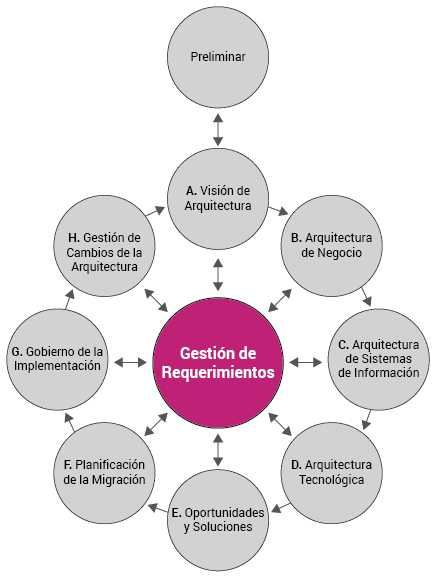
\includegraphics[scale=0.5]{figuras/5}
    	\captionsetup{width=.95\textwidth}
    	\caption{El ciclo del Modelo de Desarrollo de la Arquitectura}
    	\label{figura5}
    \end{figure}
    
    El ADM se aplica iterativamente durante todo el proceso, entre las diferentes Fases, y dentro de ellas. Durante todo el ciclo del ADM se debe realizar una validación frecuente de los resultados respecto a los requerimientos originales, tanto aquellos del ciclo completo del ADM como los de la Fase particular del proceso. Esta validación debe reconsiderar el alcance, los detalles, el plan y los hitos. Cada Fase debe considerar los activos producidos a partir de las iteraciones anteriores del proceso y los activos externos de mercado, así como otros marcos de referencia o modelos. \\
    
    El ADM apoya el concepto de iteración en tres niveles:
    \begin{itemize}
    	\itemcolor{azull}
    	\item \textbf{Ciclo alrededor del ADM:} El ADM se presenta de manera circular indicando que la finalización de una Fase de trabajo en la arquitectura alimenta directamente las Fases subsecuentes de trabajo en la arquitectura.
    	\item \textbf{Iteración entre Fases:} TOGAF describe el concepto de la iteración a través de Fases (por ejemplo, volviendo a la Arquitectura de Negocio posteriormente a la finalización de la Arquitectura Tecnológica).
    	\item \textbf{Ciclo alrededor de una Fase individual:} TOGAF apoya la ejecución repetida de las actividades dentro de una Fase individual del ADM como una técnica para elaborar contenido arquitectónico.
   \end{itemize}
   
   \begin{table}[H]
   	\centering
   	\begin{tabular}{p{3.5cm}p{8.5cm}}
   		\hline
   		\rowcolor[HTML]{0073a1}
   		{\color[HTML]{FFFFFF}\textbf{Fase de ADM}} & {\color[HTML]{FFFFFF}\textbf{Actividad}} \\
   		\hline
   		\textbf{Gestión de Requerimientos} & Cada etapa de un proyecto de TOGAF está basada en los requerimientos del negocio, incluyendo su validación.
   		Los requerimientos se identifican, se almacenan y se gestionan al ingreso y egreso de las fases relevantes del ADM, las cuales eliminan, abordan, y priorizan los requerimientos. \\ \hline
   		\textbf{A. Visión de arquitectura} & Establece el alcance, las limitaciones y expectativas de un proyecto de TOGAF. Crea la Visión de la Arquitectura. Identifica a los Interesados. Valida el contexto de negocio y crea la Declaración de Trabajo de Arquitectura. Obtiene aprobaciones. \\ \hline
   		\textbf{B. Arquitectura de Negocio C. Arquitecturas de sistemas de información D. Arquitectura tecnológica} & Desarrolla arquitecturas en cuatro dominios:
   		    \begin{enumerate}
   		    	\itemcolor{azull}
   		    	\item Negocio
   		    	\item Sistemas de Información - Aplicaciones
   		    	\item Sistemas de Información - Datos
   		    	\item Tecnología
   		    \end{enumerate}
   		En cada caso, desarrolla la Arquitectura de la línea de base y de destino y analiza las brechas entre ambas. \\  \hline
   		\textbf{E. Oportunidades y soluciones} & Realiza la planificación de la implementación inicial y la identificación de medios de entrega para los Bloques de Construcción identificados en las Fases anteriores. Determina si se requiere un enfoque incremental, y si asi fuera, identifica las Arquitecturas de Transición. \\ \hline
   		\textbf{F. Planificación de la migración} & Desarrolla el Plan detallado de Implementación y Migración que aborda cómo moverse de la Arquitectura de la Linea de Base a la Arquitectura de Destino. \\ \hline
   		\textbf{G. Gobierno de la Implementación} & Proporciona supervisión arquitectónica para la implementación. Prepara y publica Contratos de Arquitectura. Asegura que el proyecto de implementación esté en conformidad con la arquitectura. \\ \hline
   		\textbf{H. Gestión de cambios de la Arquitectura} & Proporciona seguimiento continuo y un proceso de gestión de cambios para asegurar que la arquitectura responda a las necesidades de la empresa y que se maximice el valor de la arquitectura para el negocio. \\
   		\bottomrule
   	\end{tabular}
   	\captionsetup{width=.95\textwidth}
   	\caption{Actividades del Método de Desarrollo de la arquitectura por Fase}
   	\label{tabla2} 
  \end{table}

\section{Archimate 2.1}
ArchiMate nace como un lenguaje de modelado de arquitecturas empresariales el cual tiene como objetivo proveer una representación uniforme de los diagramas que describen la arquitectura empresarial de una organización, permitiendo comprender las diferentes áreas o capas empresariales: estrategia, negocio, información, aplicaciones e infraestructura tecnológica; describiendo los diferentes dominios, relaciones, dependencias e incorporando el concepto de orientación a servicios. \\

El principal elemento en esta metodología es el servicio, que está definido como una unidad de funcionalidad que un actor (sistema o una organización) pone a disposición del ambiente de trabajo. Se adopta otro concepto ya existente: el concepto de arquitectura en capas. En una arquitectura orientada a servicios, cada capa proporciona servicios que pueden ser consumidos por capas de nivel superior, y cada capa utiliza los servicios proporcionados por capas de nivel inferior. \\
  
  \subsection{Versiones}
  Desde el año 2008 que la propiedad y los derechos de la arquitectura ArchiMate fueron transferidos al Open Group, por parte del consorcio de Universidades, empresas y el Gobierno holandés, se han publicado tres versiones de la arquitectura: ArchiMate 1.0, lanzada el año 2008 como un estándar técnico; ArchiMate 2.0, lanzada el año 2012 como un estándar; ArchiMate 2.1, en el año 2013, constituye la última versión lanzada como actualización a la versión 2.0, donde se considerando comentarios de la comunidad que aplicaban el estándar. \\
  
  La primera versión, ArchiMate 1.0, fue considerada como ya un estándar formal técnico teniendo como base lo realizado por el equipo de desarrollo del estándar. Cabe recalcar que este equipo tomó como referencia a otro estándar el de la IEEE 1471, el mismo que es utilizado para describir el diseño de una arquitectura de software. Este estándar técnico describe ArchiMate como un lenguaje que complementa al marco de trabajo (framework) TOGAF, proporcionado un juego de conceptos y definiciones que permiten representar a través de un leguaje unificado y de representación gráfica un diseño de arquitectura empresarial basado en el framework TOGAF. Se plantea el lenguaje ArchiMate como una correspodencia a las principales vistas que son definidas en la arquitectura TOGAF ADM (ADM - Architecture Develppment Method), específicamente no se hace uso de todas las vistas que menciona TOGAF, como se ilustra en la Figura 1, estás son alineadas a las tres capas que establece el estándar ArchiMarte: Business, Application, Technology. La no coincidencia de todas las capas de ArchiMate con TOGAF denota que el lenguaje está basado en el framework, el cual sí amplia y considera aspectos mucho más profundos concernientes a la arquitectura empresarial, decisiones estratégicas y de dirección. ArchiMate ofrece más un estándar formal donde se aterrizan en un diseño y un lenguaje esquemas donde se permite desarrollar la arquitectura empresarial del cual se derivarán procedimientos más operativos. \\
  
  ArchiMate 2.0, es lanzada en el año 2012 oficialmente como un estándar que conserva gran parte de su versión anterior (1.0) pero en esta ya se incluyen retroalimentaciones por parte de los usuarios del estándar, agregando así nuevas características. Esta nueva versión aparecen dos extensiones: Motivación, e Implementación y Migración. La primera considera aspectos de modelamiento de los interesados, manejos de cambios, objetivos del negocio, principios y requerimientos, se alinea principalmente a la fase inicial de las vistas de TOGAF. La extensión de Implementación y Migración, está diseñada para el manejo del portafolio del proyecto, análisis de brecha, transiciones y planes de migración, principalmente está enfocada a las fases finales de TOGAF. Ambas extensiones incluyen nuevos conceptos que dan atención a las inquietudes y experiencias de los practicantes del estándar en su versión anterior. Así tenemos los conceptos de Ubicación, que brinda un punto de vista conceptual que puede ser asignado a los elementos estructurales e indirectamente también determina sus comportamientos; y la de Función de Infraestructura, que modela el comportamiento interno de un nodo dentro de la capa de tecnología, esto permite mejorar la consistencia de la capa de tecnología con las otras dos capas (Negocios y Aplicación). \\
  
  La más reciente versión de ArchiMate es la 2.1, lanzada el año 2013, esta conserva la gran mayoría de características de su versión anterior (2.0), el motivo de su actualización se debe al direccionamiento de los comentarios de los usuarios que por años han venido usando haciendo que los mismos sean considerados y han constituido de aportes para brindar de mayores detalles y aclaraciones a los aspectos definidos por el estándar.
  
 \begin{figure}[H]
   	\centering
   	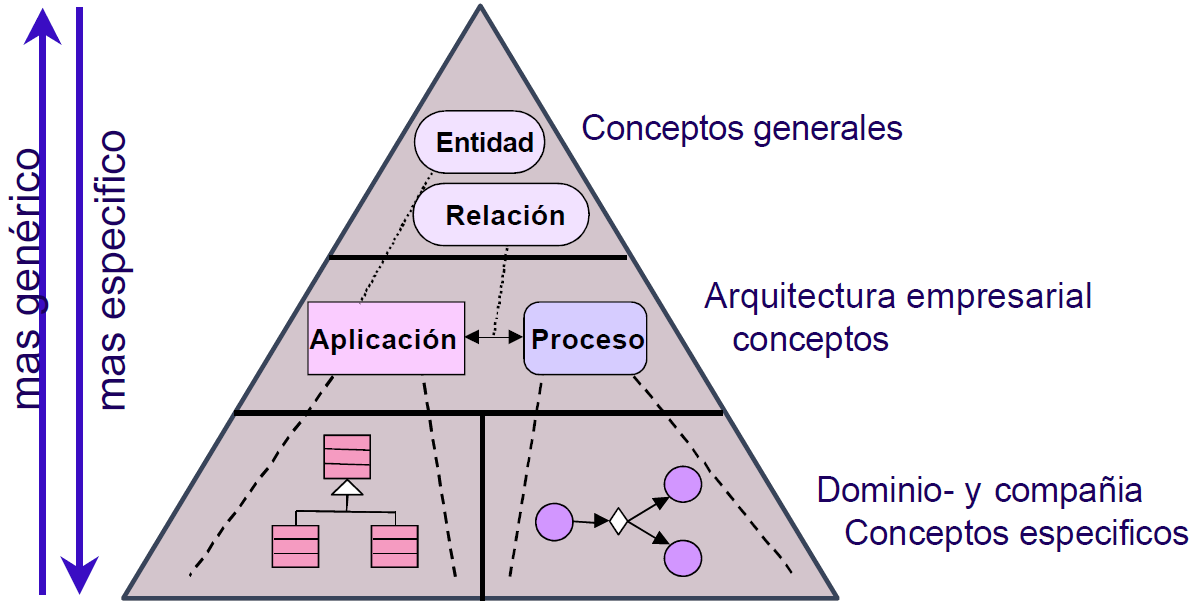
\includegraphics[scale=0.3]{figuras/6}
   	\captionsetup{width=.95\textwidth}
   	\caption{Metamodelos y diferentes niveles de especificación}
   	\label{figura6}
 \end{figure}
  
  \subsection{Conceptos centrales}
  El lenguaje central consiste de tres tipos de elementos:
  \begin{enumerate}
  	\itemcolor{azull}
  	\item \textbf{Elementos de estructura activa} Es una entidad capaz de ejercer comportamientos, tales como los actores del negocio, componentes de aplicación
  	\item \textbf{Elementos de comportamiento} Es una unidad de actividad ejecutada por uno o más elementos de estructura activa.
  	\item \textbf{Elementos de estructura pasiva} Es un objeto sobre el cual se ejecuta un comportamiento.
  	\item \textbf{Servicio} Es una unidad de funcionalidad que el sistema provee.
  	\item \textbf{Interfaz} Es el punto de acceso donde uno o más servicios son hechos disponibles al entorno. Provee una vista externa sobre el proveedor de servicio y oculta su estructura interna.
  	\item Para nombrar los roles de las interrelaciones, se utiliza una convención similar a la de UML(pero usando verbos en lugar de sustantivos).
  	\item Si no se muestra cardinalidad alguna al final de un interrelación, se asume una 0..* (cero o más).
  \end{enumerate}

  Estos elementos tienen como inspiración el lenguaje natural donde una sentencia tiene un sujeto (estructura activa), un verbo (comportamiento) y un predicado (estructura pasiva)
  
     \begin{figure}[H]
     	\centering
     	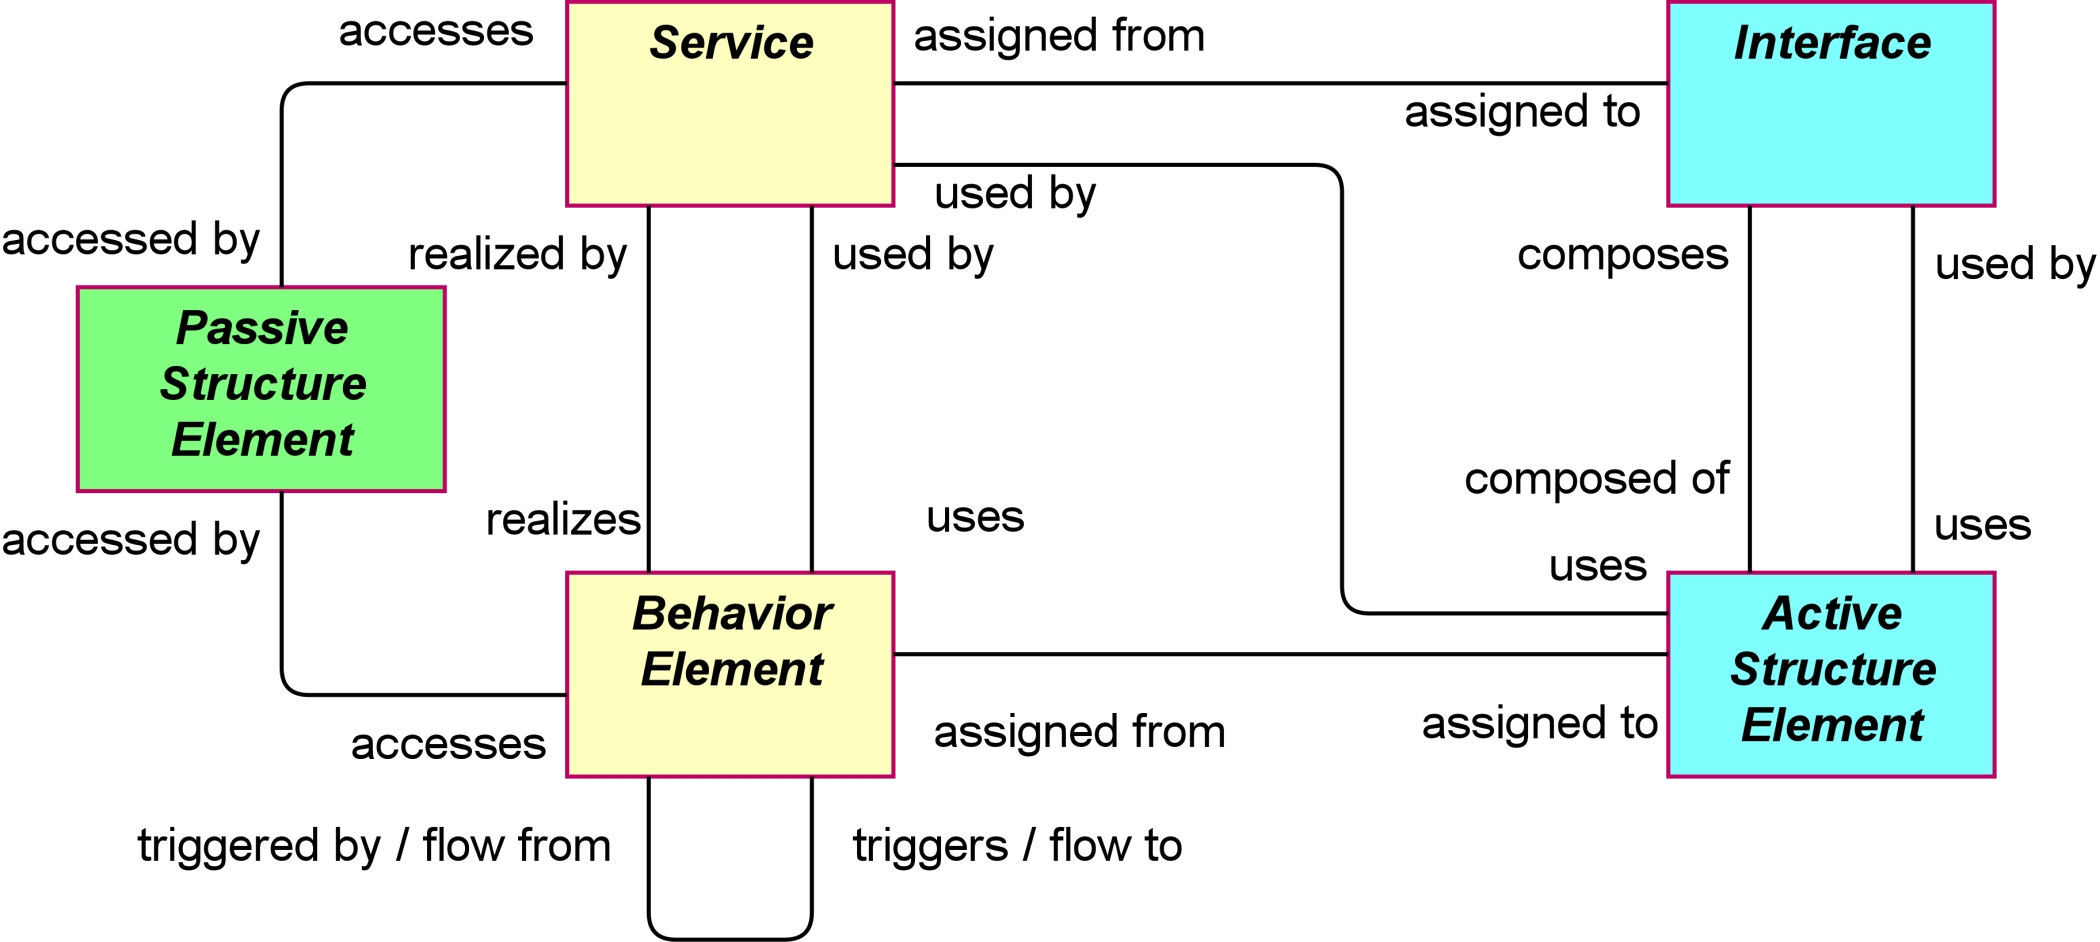
\includegraphics{figuras/7}
     	\captionsetup{width=.95\textwidth}
     	\caption{Conceptos básicos de ArchiMate}
     	\label{figura7}
     \end{figure}
  
  \subsection{Colaboración e interacción}
  Si vamos a un nivel más profundo en la estructura del lenguaje, se distingue entre el comportamiento que es realizado por un elemento de estructura única (Ejemplo: actor, rol, componentes, etc.), o comportamiento colectivo (Interacción) que se realiza por una colaboración de varios elementos de la estructura.
  
  \begin{description}
  	\item[Colaboración] Es una (temporal) agrupación (o agregación) de dos o más elementos de estructura, trabajando juntos para realizar algún comportamiento colectivo. Este comportamiento colectivo puede ser modelado como una interacción.
  	\item[Interacción] Es una unidad de comportamiento llevada a cabo por una colaboración de dos o más elementos de estructura.
  \end{description}
 
  \begin{figure}[H]
   	\centering
   	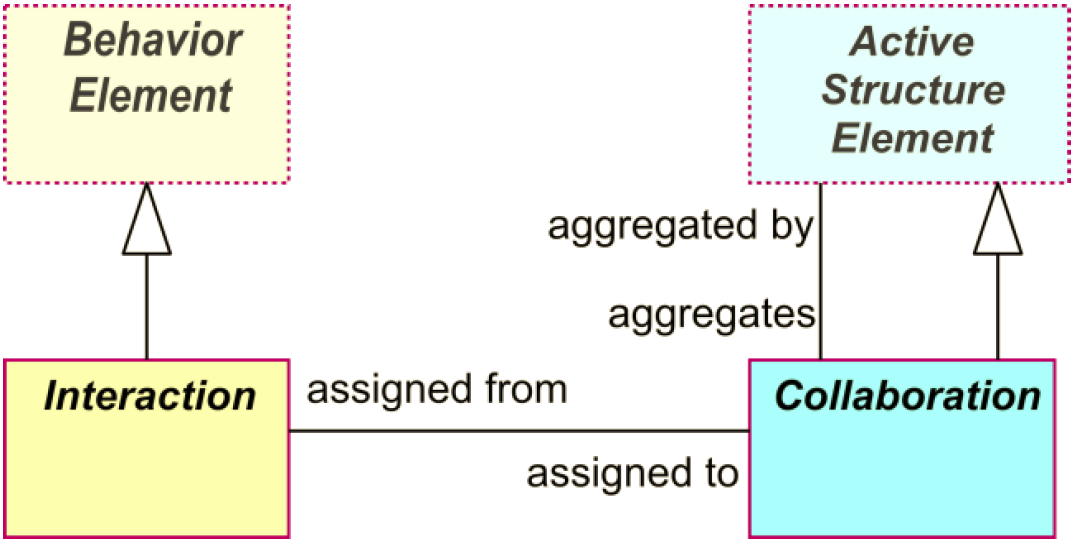
\includegraphics[scale=0.25]{figuras/8}
   	\captionsetup{width=.95\textwidth}
   	\caption{Colaboración e interacción}
   	\label{figura8}
  \end{figure}
  
  \subsection{Relaciones}
  Al lado de los conceptos fundamentales antes reseñadas, ArchiMate contiene un conjunto básico de las relaciones. Varias de estas relaciones han sido adoptadas a partir de conceptos de relación correspondientes que se producen en normas existentes. Relaciones tales como la composición, la agregación, asociación y especialización se toman de UML 2.0, mientras que la activación se utiliza en muchos procesos de negocio lenguajes de modelado.
  
  \subsection{Capas}
  En ArchiMate, hay tres diferentes capas para tres niveles diferentes en una arquitectura empresarial:
  
  \begin{enumerate}
  	\itemcolor{azull}
  	\item \textbf{Capa empresarial} La capa de negocio ofrece productos y servicios para clientes externos. Estos servicios están implementados internamente por los procesos de negocios y ejecutados por actores de negocio.
  	\item \textbf{Capa de aplicación} La capa de aplicación es compatible con la capa de negocio por servicios de aplicaciones implementados por software.
  	\item \textbf{Capa de Tecnología} La capa de tecnología proporciona los servicios de infraestructura que son necesarios para ejecutar aplicaciones (software). Son implementados por computadores y la comunicación del hardware y software del sistema.
  \end{enumerate}
  
  \subsection{Marco de referencia}
Los aspectos y capas identificadas en los apartados anteriores se pueden organizar como un marco de nueve celdas, es importante darse cuenta de que la clasificación de conceptos basados en aspectos y capas es sólo uno y es imposible definir un límite estricto entre los aspecto capas, porque los conceptos que enlazan los diferentes aspectos y capas juegan un papel central en una arquitectura coherente. El trabajo de un arquitecto de la empresa toca varios aspectos, no expresamente contemplados en el marco ArchiMate. Dominios conceptuales, son:
  \begin{itemize}
  	\itemcolor{azull}
  	\item Objetivos, principios y requisitos
  	\item Riesgos y seguridad
  	\item Gobierno
  	\item Políticas y reglas de negocio
  	\item Costos
  	\item Rendimiento
  	\item Planificación y evolución
  \end{itemize}
  
  \begin{figure}[H]
   	\centering
   	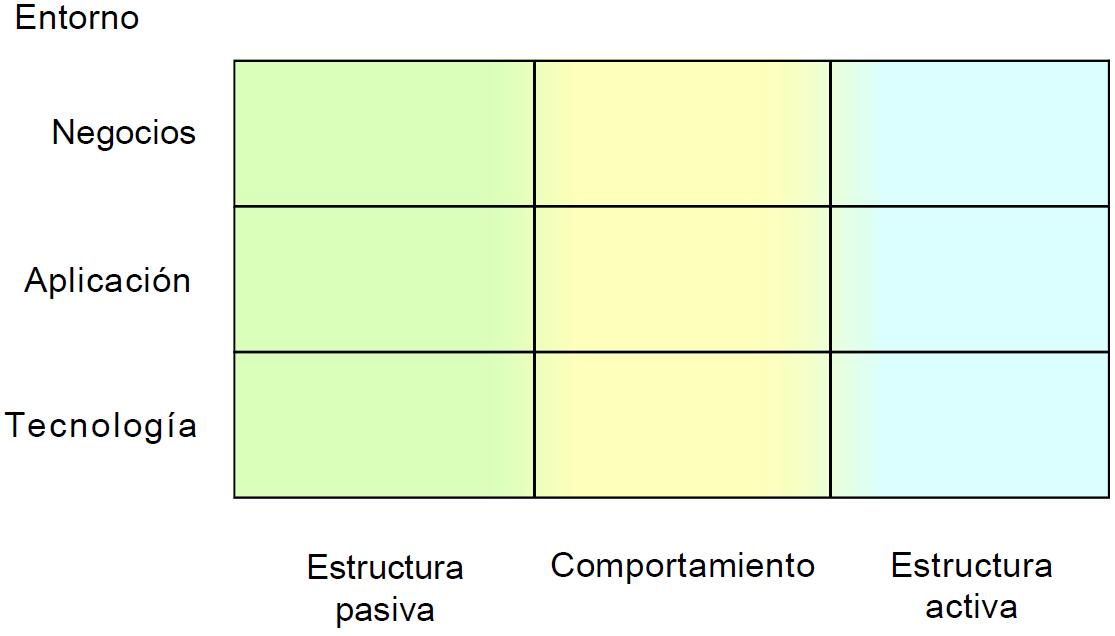
\includegraphics[scale=0.30]{figuras/9}
   	\captionsetup{width=.95\textwidth}
   	\caption{Estructura de la Arquitectura}
   	\label{figura9}
  \end{figure}

  \subsection{Motivación}
  Archimate añade los conceptos de motivación, como objetivo, principio y requisito. Un elemento de motivación se define como un elemento que proporciona el contexto o la razón que está detrás de la arquitectura de la empresa. \\
  
  La gestión de requisitos es una actividad importante en el proceso de diseño y gestión de las arquitecturas empresariales. La metas de las diversas partes interesadas son la base de cualquier cambio en una organización. Estos objetivos deben ser traducidos a los requisitos sobre la arquitectura de la organización. Esta arquitectura debería reflejar cómo los requisitos son realizados por los servicios, procesos y aplicaciones de software en las operaciones del día a día. Por lo tanto, la calidad de la arquitectura está determinada en gran medida por la capacidad de capturar y analizar los objetivos y requisitos pertinentes, el grado en que puede ser realizado por la arquitectura, y la facilidad con que objetivo y los requisitos se puede cambiar. \\
  
  Principios y requerimientos están fuertemente relacionados. Los principios son normas y directrices generales que ayudan a informar y apoyar la forma en que una organización se marca sobre el cumplimiento de su misión. En contraste, las limitaciones de los requisitos dan forma a un diseño específico de la arquitectura empresarial. Esto corresponde a la distinción entre dos interpretaciones generales:
  \begin{itemize}
  	\itemcolor{azull}
  	\item Como la estructura de una organización en términos de sus componentes y sus relaciones
  	\item Como un conjunto de principios que se deben aplicar a dicha estructura.
  \end{itemize}
  El alcance de la primera interpretación se refiere a un solo diseño de la organización, mientras que el segundo se refiere a cualquier diseño posible. Los requisitos están asociados con la primera interpretación. En su lugar, los principios son independientes de un diseño específico y tienen que especializarse en las necesidades y en el proceso de diseño de la arquitectura de la organización. \\
  
  La gestión de requisitos inadecuada es una de las principales causas de daños y fallas en los proyectos informáticos, por exceder los presupuestos o plazos, por no entregar los resultados esperados. Por lo tanto, el proceso de gestión de requisitos y el proceso de desarrollo de la arquitectura necesitan estar bien alineados, y la trazabilidad deben mantenerse entre las necesidades de los elementos arquitectónicos que dan cuenta a estos requisitos.
 
  \begin{figure}[H]
   	\centering
   	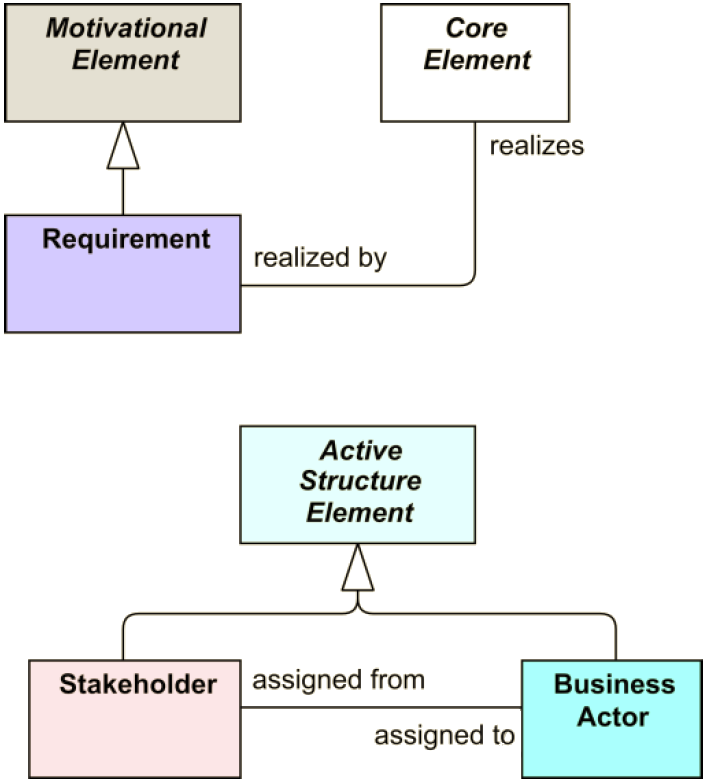
\includegraphics[scale=0.30]{figuras/10}
   	\captionsetup{width=.95\textwidth}
   	\caption{Relación entre los elementos básicos de motivación en ArchiMate}
   	\label{figura10}
  \end{figure}
  
  \subsection{Implementación y Migración}
  La extensión de implantación y migración de ArchiMate añade conceptos para apoyar las fases finales de ADM, relacionados con la implementación y migración de arquitecturas: Fase E (Oportunidades y Soluciones), Fase F (planeamiento de migración), y la Fase G (Gobierno de Aplicación). \\
  
  Esta extensión incluye conceptos para el modelado de los programas y proyectos de aplicación que soportan los programas, el portafolio y la gestión de proyectos. Conceptos que son específicos para uno de estos métodos no son parte de la extensión, pero se pueden definir como la especialización de los conceptos genéricos. De esta manera, el conjunto de conceptos y relaciones que se define en la extensión se mantiene a un mínimo.

  \begin{figure}[H]
  	\centering
   	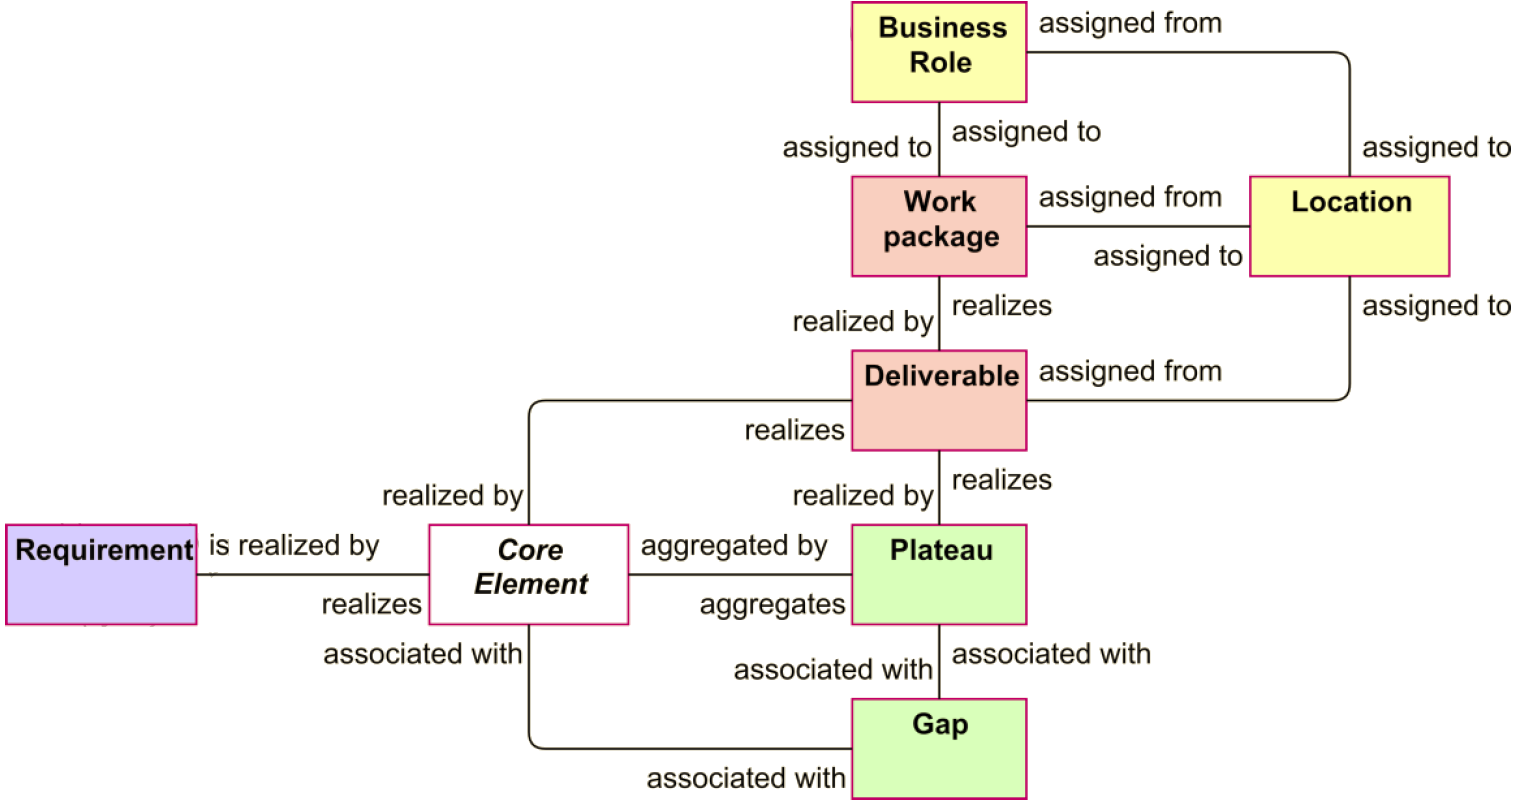
\includegraphics[scale=0.27]{figuras/11}
   	\captionsetup{width=.95\textwidth}
   	\caption{Relaciones entre la motivación, Core, Implementación y Migración}
   	\label{figura11}
  \end{figure}

   \subsection{Archimate: Su relación con TOGAF}
   El lenguaje ArchiMate, tal como se describe en la Norma Técnica, complementa TOGAF, ya que proporciona un conjunto independiente de los proveedores de los conceptos, incluyendo una representación gráfica, que ayuda a crear un modelo integrado coherente "por debajo de la línea de flotación", que puede ser representado en forma de puntos de vista TOGAF. \\
   
   Aunque algunos de los puntos de vista que se definen en TOGAF son difíciles de hacer corresponder con los puntos de vista ArchiMate, el idioma ArchiMate y sus técnicas de análisis sí apoyan los conceptos abordados en estos puntos de vista. Si bien no hay correlación de uno a uno entre ellos, todavía hay una buena cantidad de correspondencia entre los puntos de vista ArchiMate y los puntos de vista que se definen en TOGAF. Aunque los puntos de vista correspondientes de ArchiMate y TOGAF no necesariamente tienen la misma cobertura, podemos ver que muchos puntos de vista de ambos métodos abordan en gran medida los mismos problemas.
   
   TOGAF y ArchiMate pueden ser fácilmente utilizados en conjunto y parecen cubrir gran parte de lo mismo, aunque con algunas diferencias en el alcance y enfoque.
   
     \begin{figure}[H]
     	\centering
     	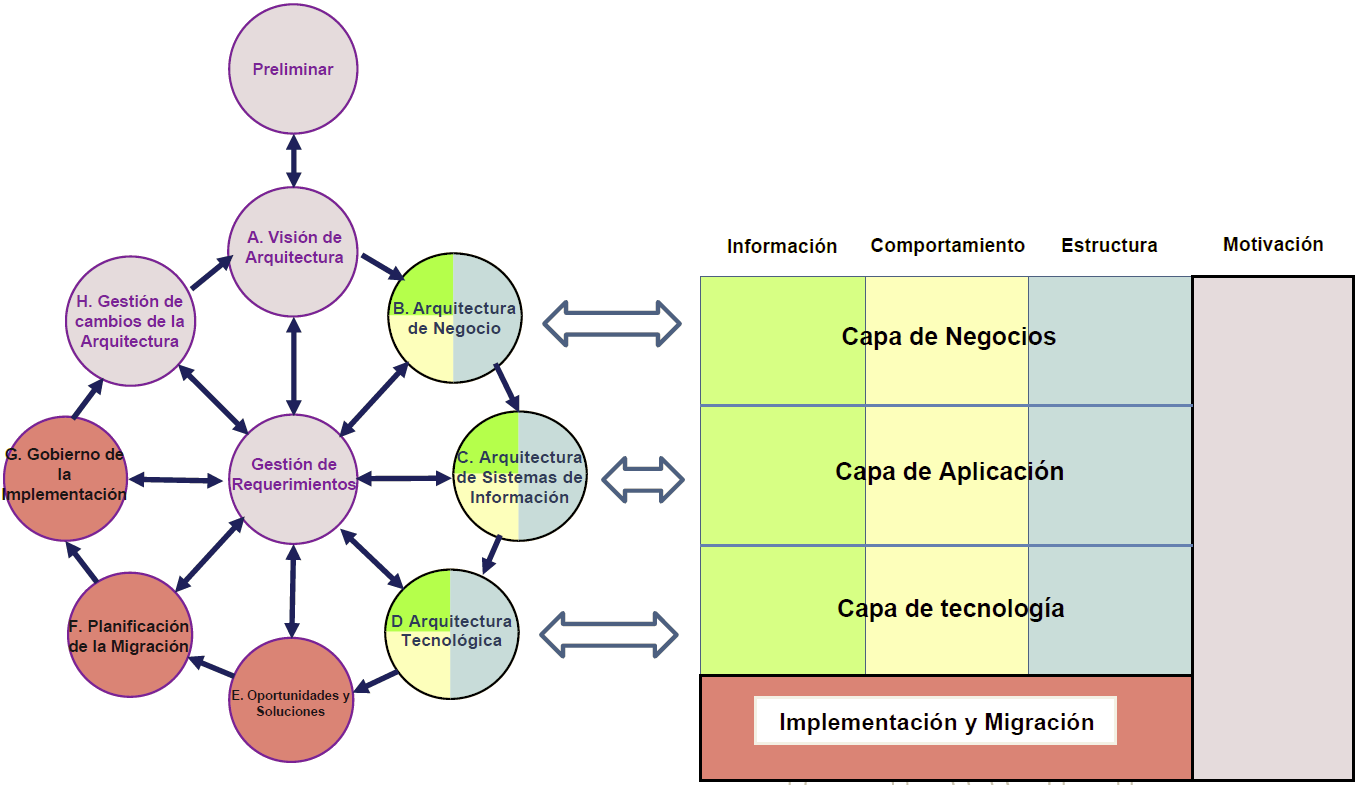
\includegraphics[scale=0.29]{figuras/12}
     	\captionsetup{width=.95\textwidth}
     	\caption{Correspondencia entre ArchiMate (incluyendo extensiones) y TOGAF}
     	\label{figura12}
     \end{figure}

\chapter{Patrones}
\label{chap:patrones}
\textit{The first chapter introduces fluorescence-based DNA technology and highlights the motivation of the research conducted in the thesis}
\vfill
\minitoc
\newpage

\section{Programación Orientada a objetos}
La POO es un paradigma de la programación de computadores; esto hace referencia al conjunto de teorías, estándares, modelos y métodos que permiten organizar el conocimiento, proporcionando un medio bien definido para visualizar el dominio del problema e implementar en un lenguaje de programación la solución a ese problema. \\

La POO se basa en el modelo objeto donde el elemento principal es el objeto, el cual es una unidad que contiene todas sus características y comportamientos en sí misma, lo cual lo hace como un todo independiente pero que se interrelaciona con objetos de su misma clase o de otras clase, como sucede en el mundo real. \\

Una ventaja de la POO frente al paradigma algorítmico es la facilidad que brinda a través de sus herramientas, de concebir, analizar, modelar, diseñar e implementar el mundo real de manera fiel a como se presenta en la realidad; el paso que hay desde la concepción y asimilación del problema hasta la implementación del mismo es un proceso que se hace de manera casi natural. Esto porque el mundo está lleno de objetos reales, los cuales se pueden representar como tales en una solución computarizada.

\section{Patrones de software}
Los patrones para el desarrollo de software son uno de los últimos avances de la Tecnología Orientada a Objetos. Los patrones son una forma literaria para resolver problemas de
ingeniería del software, que tienen sus raíces en los patrones de la arquitectura. \\

Los diseñadores y analistas de software más experimentados aplican de forma intuitiva algunos criterios que solucionan los problemas de manera elegante y efectiva. La ingeniería del
software se enfrenta a problemas variados que hay que identificar para poder utilizar la misma solución (aunque matizada) con problemas similares. \\

El objetivo de los patrones es crear un lenguaje común a una comunidad de desarrolladores para comunicar experiencia sobre los problemas y sus soluciones.

  \subsection{Definiciones}
  Los diferentes autores han dado diversas definiciones de lo que es un patrón software.
  \begin{itemize}
  	\itemcolor{azull}
  	\item \textit{Dirk Riehle y Heinz Zullighoven:} \\
  	“Un patrón es la abstracción de una forma concreta que puede repetirse en contextos específicos.”.
 	\item \textit{Richard Gabriel:} \\
  	“  Cada patrón es una regla de tres partes, la cual expresa una relación entre un cierto contexto, un conjunto de fuerzas que ocurren repetidamente en ese contexto y una cierta configuración software que permite a estas fuerzas resolverse por si mismas.”.
  \end{itemize}
  
  \subsection{Clases de patrones software}
  Existen diferentes ámbitos dentro de la ingeniería del software donde se pueden aplicar los patrones:
  \begin{enumerate}
  	\itemcolor{azull}
  	\item \textbf{Patrones de Arquitectura:} Expresa una organización o esquema estructural fundamental para sistemas software. Proporciona un conjunto de subsistemas predefinidos, especifica sus responsabilidades, e incluye una guía para organizar las relaciones entre ellos.
  	\item \textbf{Patrones de Diseño:} Proporciona un esquema para refinar los subsistemas o componentes de un sistema software, o las relaciones entre ellos. Describe
  	estructuras repetitivas de comunicar componentes que resuelven un problema de diseño en un contexto particular.
  	\item \textbf{Patrones de Programación:} Un idioma es un patrón de bajo nivel de un lenguaje de programación específico. Describe como implementar aspectos de componentes o de las relaciones entre ellos utilizando las facilidades del lenguaje de programación dado.
  	\item \textbf{Patrones de Análisis:} Describen un conjunto de prácticas que aseguran la obtención de un buen modelo de un problema y su solución.
  	\item \textbf{Patrones Organizacionales:} Describen la estructura y prácticas de las organizaciones.
  \end{enumerate}
  
  \section{Patrones de Diseño}
  Los patrones de diseño tienen un cierto nivel de abstracción. Los patrones de diseño no son
  diseños tales como la realización de listas y tablas hash que pueden ser codificadas en clases y reutilizadas. Un algoritmo puede ser un ejemplo de implementación de un patrón, pero es demasiado incompleto, específico y rígido para ser un patrón. Una regla o heurística puede
  participar en los efectos de un patrón, pero un patrón es mucho más. Los patrones de diseño
  son descripciones de las comunicaciones de objetos y clases que son personalizadas para
  resolver un problema general de diseño en un contexto particular. \\
  
  Un patrón de diseño nombra, abstrae e identifica los aspectos clave de un diseño estructurado, común, que lo hace útil para la creación de diseños orientados a objetos   reutilizables. Los patrones de diseño identifican las clases participantes y las instancias, sus papeles y colaboraciones, y la distribución de responsabilidades. Cada patrón de diseño se
  enfoca sobre un particular diseño orientado a objetos. Se describe cuando se aplica, las características de otros diseños y las consecuencias y ventajas de su uso. \\
  
  Los patrones de diseño se pueden utilizar en cualquier lenguaje de programación orientado a objetos, adaptando los diseños generales a las características de la implementación particular.
  
  \subsection{Clasificación de los patrones de diseño}
  Dado que hay muchos patrones de diseño necesitamos un modo de organizarlos. En esta sección clasificamos los patrones de diseño de tal forma que podamos referirnos a familias de patrones relacionados. La clasificación nos ayuda a saber lo que hace un patrón. Según el libro “Patterns in Java (Volume 1)” existen seis categorías:
  
  \subsubsection{Fundamentales}
  Los patrones de esta categoría son los más fundamentales e importantes patrones de diseño
  conocidos. Estos patrones son utilizados extensivamente en otros patrones de diseño.
  
  \subsubsection{Creación}
  Los patrones de creación muestran la guía de cómo crear objetos cuando sus creaciones requieren tomar decisiones. Estas decisiones normalmente serán resueltas dinámicamente decidiendo que clases instanciar o sobre que objetos un objeto delegará responsabilidades. \\
  
  A menudo hay varios patrones de creación que puedes aplicar en una situación. Algunas  veces se pueden combinar múltiples patrones ventajosamente. En otros casos se debe elegir  entre los patrones que compiten.
  
  \subsubsection{Partición}
  Los patrones de esta categoría proveen la guía sobre como dividir actores complejos y casos de uso en múltiples clases.
  
  \subsubsection{Estructurales}
  Los patrones de esta categoría describen las formas comunes en que diferentes tipos de objetos pueden ser organizados para trabajar unos con otros.
  
  \subsubsection{Comportamiento}
  Los patrones de este tipo son utilizados para organizar, manejar y combinar comportamientos.
  
  \subsubsection{Concurrencia}
  Los patrones de esta categoría permiten coordinar las operaciones concurrentes. Estos patrones se dirigen principalmente a dos tipos diferentes de problemas:
  \begin{enumerate}
  	\itemcolor{azull}
  	\item \textbf{Recursos compartidos:}
  	Cuando las operaciones concurrentes acceden a los mismos datos o otros tipos de recursos compartidos, podría darse la posibilidad de que las operaciones interfirieran unas con otras si ellas acceden a los recursos al mismo tiempo. Para garantizar que cada operación se ejecuta correctamente, la operación debe ser protegida para acceder a los recursos compartidos en solitario. Sin embargo, si las operaciones están completamente protegidas, entonces podrían bloquearse y no ser capaces de finalizar su ejecución.
  	\item \textbf{Secuencia de operaciones:}
  	Si las operaciones son protegidas para acceder a un recurso compartido una cada vez, entonces podría ser necesario garantizar que ellas acceden a los recursos compartidos en un orden particular. Por ejemplo, un objeto nunca será borrado de una estructura de datos antes de que esté sea añadido a la estructura de datos.
  \end{enumerate}
  	
  \begin{table}[H]
  	\centering
  	\begin{tabular}{p{6cm}|p{6cm}}
  		\hline
  		\rowcolor[HTML]{0073a1}
  		{\color[HTML]{FFFFFF} \textbf{Fundamentales}} & {\color[HTML]{FFFFFF}\textbf{De Creación}} \\
  		\hline
  		\begin{itemize}
  			\itemcolor{azull}
  			\item Delegation
  			\item Interface
  			\item Unmitable
  			\item Marker Interface
  			\item Proxy
  		\end{itemize} &
  		\begin{itemize}
  			\itemcolor{azull}
  			\item Factory Method
  			\item Abstract Factory
  			\item Builder
  			\item Prototype
  			\item Singleton
  			\item Object Pool
  		\end{itemize} \\
  		\hline
  		\rowcolor[HTML]{0073a1}
  		{\color[HTML]{FFFFFF} \textbf{De Partición}} & {\color[HTML]{FFFFFF}\textbf{Estructurales}} \\
  		\hline
  		\begin{itemize}
  			\itemcolor{azull}
  			\item Layered Initialization
  			\item Filter
  			\item Composite
  		\end{itemize} &
  		\begin{itemize}
  			\itemcolor{azull}
  			\item Adapter
  			\item Iterator
  			\item Bridge
  			\item Facade
  			\item Flyweight
  			\item Dynamic Linkage
  			\item Virtual proxy
  			\item Decorator
  			\item Cache Management
  		\end{itemize} \\
  		\midrule
  	\end{tabular}
  \end{table}
  
  \begin{table}[H]
  	\centering
  	\begin{tabular}{p{6cm}|p{6cm}}  		
  		\hline
  		\rowcolor[HTML]{0073a1}
  		{\color[HTML]{FFFFFF} \textbf{De Comportamiento}} & {\color[HTML]{FFFFFF}\textbf{De Concurrencia}} \\
  		\hline
  		\begin{itemize}
  			\itemcolor{azull}
  			\item Chain of Responsability
  			\item Command
  			\item Little Language
  			\item Mediator
  			\item Snapshot
  			\item Observer
  			\item State
  			\item Null Object
  			\item Strategy
  			\item Template Method
  			\item Visitor
  		\end{itemize} &
  		\begin{itemize}
  			\itemcolor{azull}
  			\item Single Threaded Execution
  			\item Guarded Suspension
  			\item Balking
  			\item Scheduler
  			\item Read/Write Lock
  			\item Producer-Consumer
  			\item Two-Phase Termination
  		\end{itemize} \\
  		\bottomrule
  	\end{tabular}
  	\captionsetup{width=.95\textwidth}
  	\caption{Catalogo de Patrones de Diseño}
  	\label{tabla3} 
  \end{table}

\chapter{Colosoft}
\label{chap:coloso}
\textit{The first chapter introduces fluorescence-based DNA technology and highlights the motivation of the research conducted in the thesis}
\vfill
\minitoc
\newpage

\section{Descripción}
Coloso es una plataforma de desarrollo dirigida a la gestión integral del proceso de Ingeniería de Software que nos permite desarrollar metodologías de arquitectura empresarial. Fue desarrollado por Colosoft, una comunidad dedicada a la investigación, desarrollo e innovación en ingeniería de software. \\

El software Coloso hace parte de un conjunto de herramientas que permiten abordar el desarrollo de software en todas sus etapas. Soporta diferentes metodologías de desarrollo generando los artefactos que aplica a cada metodología especifica, Soporta las disciplinas como: Ingeniería de desarrollo, Arquitectura de software, Ingeniería de procesos de software, Desarrollo de alto nivel, Diseño de software, Ingeniería de sistemas, Análisis de sistemas, Ingeniería de software, Ingeniería de requerimientos, Patrones, Permite el modelamiento de arquitecturas empresariales y soporta los 25 puntos de vista del lenguaje Archimate.
  \begin{figure}[H]
   	\centering
   	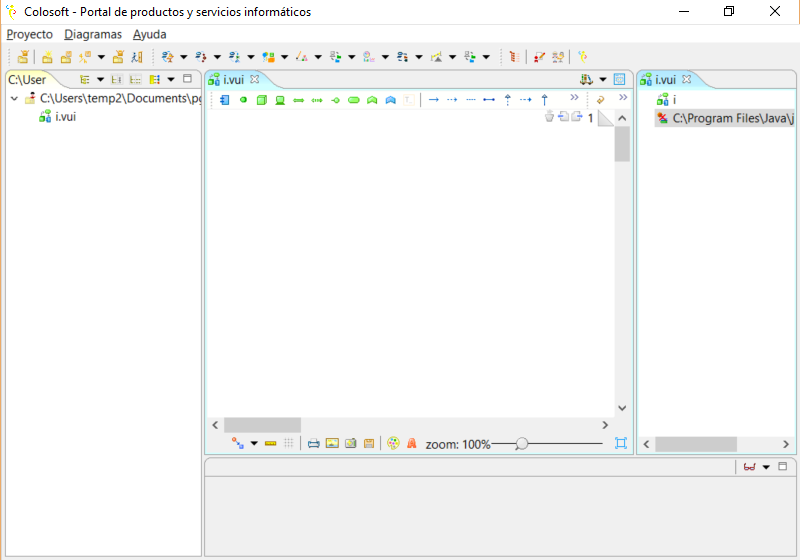
\includegraphics[scale=0.8]{figuras/13}
   	\captionsetup{width=.95\textwidth}
   	\caption{Interfaz Coloso}
   	\label{figura13}
  \end{figure}
	\part{Arquitectura Empresarial}
		\chapter{Modelo de Negocio\index{Negocio}}
\label{chap:Negocio}
\textit{En el presente capítulo se despliega el desarrollo de la Arquitectura Empresarial\index{Arquitectura Empresarial} correspondiente al Modelo de Negocio\index{Negocio} utilizando Archimate\index{Archimate}.}
\vspace{2ex}\vfill
\minitoc
\cleardoublepage

\section{Punto de Vista de la Organización\index{Organización}}
 El punto de vista de la organización se enfoca en el interior de la organización, un departamento, una red de empresas, es un punto de vista muy útil ya que permite identificar  competencias, autoridad y responsabilidades en una organización. \cite{ref9}
 
  \begin{table}[H]
	\centering
	\begin{tabular}{p{3.7cm}p{8cm}}
		\hline
		\rowcolor[HTML]{0073a1}
		{\color[HTML]{FFFFFF} \textbf{Nombre}} & {\color[HTML]{FFFFFF} \textbf{Organización\index{Organización}}} \\
		\hline
		\textbf{Stakeholder\index{Stakeholder}s} & Organización\index{Organización}, arquitectos de dominio y proceso, gerentes, empleados, accionistas \\
		\textbf{Preocupaciones} & Identificación de competencias, autoridad y responsabilidades \\
		\textbf{Propósito} & Diseñar\index{Diseñar}, decidir, informar \\
		\textbf{Nivel de Abstracción\index{Abstracción}} & Coherencia\index{Coherencia} \\
		\textbf{Capa} & Capa de negocio \\
		\textbf{Aspectos} & Activo \\
		\bottomrule
	\end{tabular}
	\captionsetup{width=.95\textwidth}
	\caption{Descripción Punto de Vista de la Organización\index{Organización} \cite{ref9}}
	\label{tabla4}
  \end{table}

  \begin{figure}[H]
 	\centering
 	
\includegraphics[scale=0.2]{figuras/14}
 	\captionsetup{width=.95\textwidth}
 	\caption{Posición del punto de vista de organización conceptualmente y marco del punto de vista \cite{ref9}}
 	\label{figura14}
  \end{figure}

  \subsection{Metamodelo\index{Metamodelo}}
  En la Figura \ref{metamodelo1} se ilustra el metamodelo perteneciente al punto de vista de organización, el cual está compuesto de los conceptos de actor, rol, interface, colaboración y localización. En este punto de vista se destaca como concepto fundamental que el actor juega un rol el cual está ubicado en una localización haciendo parte de una colaboración de negocio y se comunica con su entorno a través de una interface. \cite{ref9}
 
 \begin{figure}[H]
   \centering
   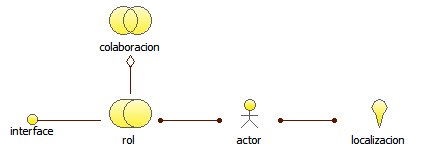
\includegraphics{metamodelos/1}
   \captionsetup{width=.95\textwidth}
   \caption{Metamodelo\index{Metamodelo} Punto de vista organización \cite{ref9}}
   \label{metamodelo1}
 \end{figure}

 \subsection{Modelo mInstituto}
 Esta vista es la interpretación sobre el organigrama en donde se representan los roles desempeñados en la empresa para el proceso de Minstituto\index{Minstituto}, cabe resaltar la importancia de identificar los roles de la estructura organizacional y su interacción que permitirá establecer las estrategias necesarias para controlar los procesos.  Como actores se reconoce al desarrollador, el analista de pruebas y el ejecutivo comercial.
  \begin{figure}[H]
   \centering
   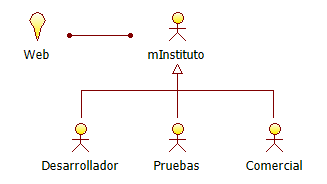
\includegraphics[scale=0.8]{modelos/1}
   \captionsetup{width=.95\textwidth}
   \caption{Modelo Punto de vista organización: minstituto}
   \label{modelo1}
  \end{figure}
  
  \section{Punto de Vista Cooperación\index{Cooperación} de Actor}
  Este punto de vista se enfoca en los actores y sus relaciones con el entorno que los cobija, es un punto de vista donde los Stakeholder\index{Stakeholder}s o interesados son la organización, los procesos y los arquitectos de dominio. La finalidad u objetivo de este punto de vista es la de diseñar, decidir e informar. \cite{ref9}
  
  \begin{table}[H]
  	\centering
  	\begin{tabular}{p{3.7cm}p{8cm}}
  		\hline
  		\rowcolor[HTML]{0073a1}
  		{\color[HTML]{FFFFFF} \textbf{Nombre}} & {\color[HTML]{FFFFFF} \textbf{Cooperación\index{Cooperación} de Actor}} \\
  		\hline
  		\textbf{Stakeholder\index{Stakeholder}s} & Organización\index{Organización}, arquitectos de dominio y proceso \\
  		\textbf{Preocupaciones} & Relación de actores con el entorno \\
  		\textbf{Propósito} & Diseñar\index{Diseñar}, decidir, informar \\
  		\textbf{Nivel de Abstracción\index{Abstracción}} & Detalle \\
  		\textbf{Capa} & Capa de negocio \\
  		\textbf{Aspectos} & Estructura\index{Estructura} Activa, Comportamiento\index{Comportamiento} \\
  		\bottomrule
  	\end{tabular}
  	\captionsetup{width=.95\textwidth}
  	\caption{Descripción Punto de Vista Cooperación\index{Cooperación} de Actor \cite{ref9}}
  	\label{tabla5}
  \end{table}
  
   \begin{figure}[H]
   	\centering
   	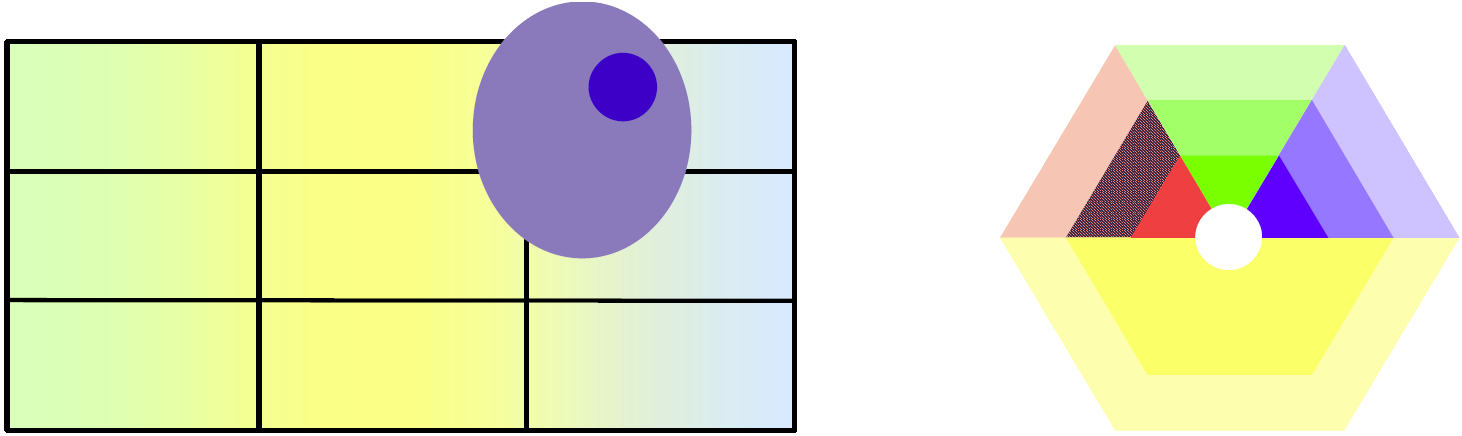
\includegraphics[scale=0.2]{figuras/15}
   	\captionsetup{width=.95\textwidth}
   	\caption{Posición del punto de vista cooperación de actor conceptualmente y marco del punto de vista \cite{ref9}}
   	\label{figura15}
   \end{figure}
  
  \subsection{Metamodelo\index{Metamodelo}}
  En la Figura \ref{metamodelo2} se ilustra el metamodelo perteneciente al punto de vista de cooperación de actor el cual esta compuesto de los conceptos de actor, rol, interface, colaboración, servicio de negocio, servicio de aplicación, interface de comunicación de aplicación y componentes de aplicación.\\
  
  En este punto de vista a el actor se le asigna un rol, el rol se compone de interfaces, a la interface se le asigna servicios y estos servicios van a una capa de aplicación a través de una interface que está conformada por componentes de aplicación y es usada por componentes de aplicación. \\
  
  Otro uso importante del punto de vista de cooperación de actor es mostrar como un número de actores de negocio cooperantes y / o componentes de aplicación juntos realizan un proceso de negocio. Por lo tanto, en esta vista, tanto actores de negocio como roles y componentes de aplicación pueden aparecer. \cite{ref9}
  
  \begin{figure}[H]
  	\centering
  	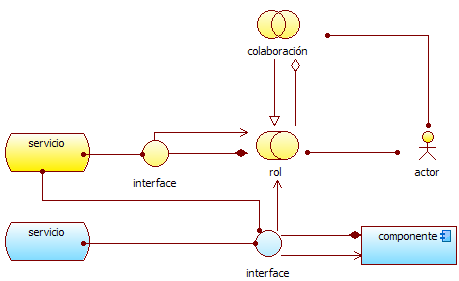
\includegraphics{metamodelos/2}
  	\captionsetup{width=.95\textwidth}
  	\caption{Metamodelo\index{Metamodelo} Punto de Vista Cooperación\index{Cooperación} de Actor \cite{ref9}}
  	\label{metamodelo2}
  \end{figure}
  
  \subsection{Modelo mInstituto}
  Para la empresa se establece una clara interacción por parte del área comercial con el cliente y retroalimentación para el equipo de proyecto, el cual se compone del área de producción, es decir, el desarrollador y el analista de pruebas, que serán los encargados de dar trámite a las solicitudes y requerimientos del cliente.
  
  \begin{figure}[H]
  	\centering
  	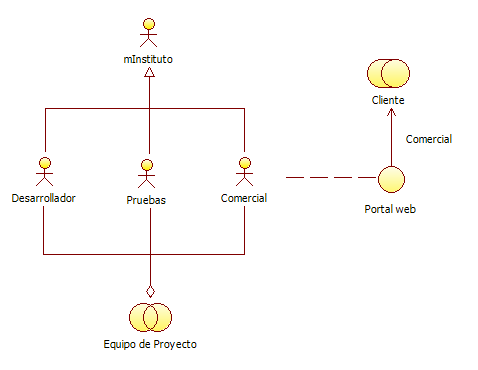
\includegraphics[scale=0.8]{modelos/2}
  	\captionsetup{width=.95\textwidth}
  	\caption{Modelo Punto de Vista Cooperación\index{Cooperación} de Actor: minstituto}
  	\label{modelo2}
  \end{figure}
 
  \section{Punto de Vista Función de Negocio\index{Negocio}}
  En este punto de vista se muestran las principales funciones de negocio de la organización y sus relaciones en términos de los flujos de información, valor, o productos entre ellas, los Stakeholder\index{Stakeholder}s o interesados son los procesos y arquitectos de dominio, administradores operacionales, tiene especial cuidado en la estructura de los procesos de negocio, su coherencia, integridad y las responsabilidades. \cite{ref9}

  \begin{table}[H]
  	\centering
  	\begin{tabular}{p{3.7cm}p{8cm}}
  		\hline
  		\rowcolor[HTML]{0073a1}
  		{\color[HTML]{FFFFFF} \textbf{Nombre}} & {\color[HTML]{FFFFFF} \textbf{Función de Negocio\index{Negocio}}} \\
  		\hline
  		\textbf{Stakeholder\index{Stakeholder}s} & Organización\index{Organización}, arquitectos de dominio y proceso \\
  		\textbf{Preocupaciones} & Identificación de competencias, identificación de actividades principales, reducción de la complejidad \\
  		\textbf{Propósito} & Diseñar\index{Diseñar} \\
  		\textbf{Nivel de Abstracción\index{Abstracción}} & Coherencia\index{Coherencia} \\
  		\textbf{Capa} & Capa de negocio \\
  		\textbf{Aspectos} & Comportamiento\index{Comportamiento} (Activo) \\
  		\bottomrule
  	\end{tabular}
   	\captionsetup{width=.95\textwidth}
   	\caption{Descripción Punto de Vista Función de Negocio\index{Negocio} \cite{ref9}}
   	\label{Tab:tabla6}
  \end{table}

  \begin{figure}[H]
   	\centering
   	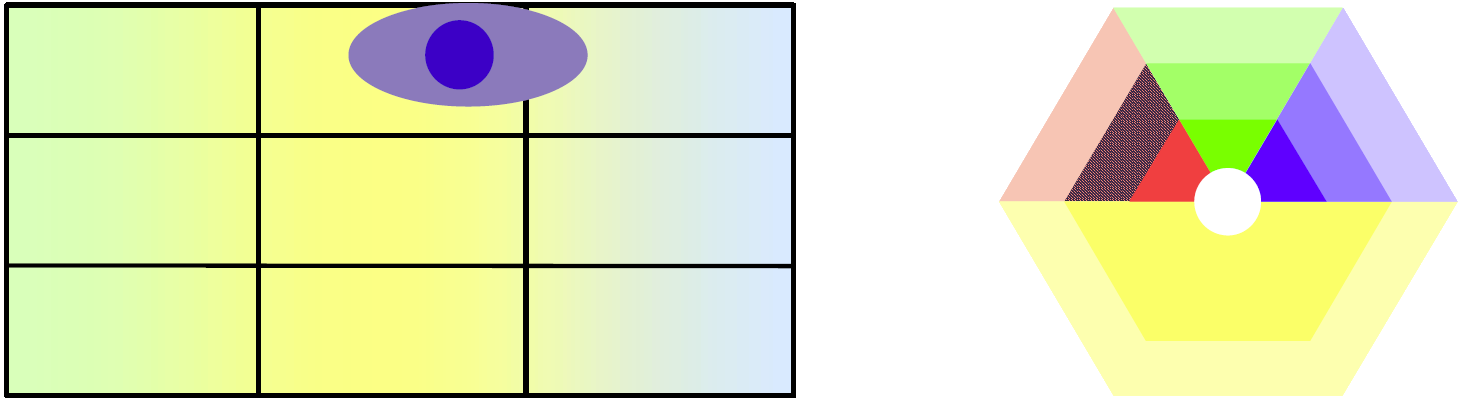
\includegraphics[scale=0.2]{figuras/16}
   	\captionsetup{width=.95\textwidth}
   	\caption{Posición del punto de vista función de negocio conceptualmente y marco del punto de vista \cite{ref9}}
   	\label{figura16}
   \end{figure}
    
   \subsection{Metamodelo\index{Metamodelo}}
   La Figura \ref{metamodelo3} muestra los conceptos de actor, rol y función; aquí se asignan tareas o funciones a estos actores, en el modelo se extrae lo que interesa, lo que se quiere capturar o tener en la mente. En este metamodelo aparecen dos tipos de relaciones el flujo y los disparos. \cite{ref9}
    
   \begin{figure}[H]
   	\centering
   	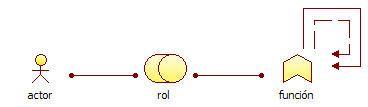
\includegraphics{metamodelos/3}
   	\captionsetup{width=.95\textwidth}
   	\caption{Metamodelo\index{Metamodelo} Punto de Vista Función de Negocio\index{Negocio} \cite{ref9}}
   	\label{metamodelo3}
   \end{figure}
    
    \subsection{Modelo mInstituto}
    En la vista se especifica la función principal de negocio la cual es la comercialización de licencias de uso del software a través de la captación de clientes por medio de material publicitario y la información que se presenta en el portal empresarial, la cual ha sido desarrollada por el diseñador.
    
    \begin{figure}[H]
    	\centering
    	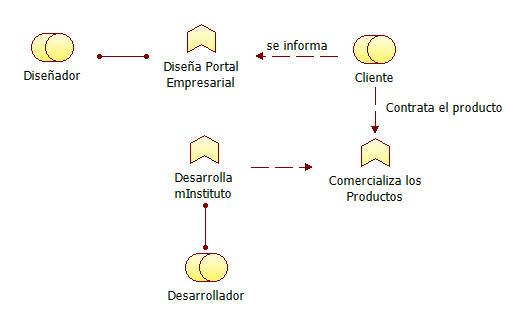
\includegraphics[scale=0.75]{modelos/3}
    	\captionsetup{width=.95\textwidth}
    	\caption{Modelo Punto de Vista Función de Negocio\index{Negocio}: minstituto}
    	\label{modelo3}
    \end{figure}

  \section{Punto de Vista Proceso\index{Proceso} de Negocio\index{Negocio}}
  El punto de vista de proceso de negocio es el encargado de mostrar una estructura de alto nivel y composición de uno o más procesos de negocio. Tiene una complejidad importante, se incorporan elementos de comportamiento se incluye el proceso y/o función de negocio como elemento central, el proceso y/o función de negocio se ve afectado por las mismas relaciones con los demás conceptos, este punto de vista llama la atención en que nos induce a las entrañas de las organizaciones porque se ve lo que ellas hacen. \cite{ref9}
  
  \begin{table}[H]
  	\centering
  	\begin{tabular}{p{3.7cm}p{8cm}}
  		\hline
  		\rowcolor[HTML]{0073a1}
  		{\color[HTML]{FFFFFF} \textbf{Nombre}} & {\color[HTML]{FFFFFF} \textbf{Proceso\index{Proceso} de Negocio\index{Negocio}}} \\
  		\hline
  		\textbf{Stakeholder\index{Stakeholder}s} & Arquitectura de dominio y proceso, Gerentes de operación \\
  		\textbf{Preocupaciones} & Estructura\index{Estructura}r los procesos del negocio, consistencia, integridad y responsabilidades \\
  		\textbf{Propósito} & Diseñar\index{Diseñar} \\
  		\textbf{Nivel de Abstracción\index{Abstracción}} & Detalle \\
  		\textbf{Capa} & Capa de negocio \\
  		\textbf{Aspectos} & Comportamiento\index{Comportamiento} (Activo), (Pasivo) \\
  		\bottomrule
  	\end{tabular}
  	\captionsetup{width=.95\textwidth}
  	\caption{Descripción punto de vista proceso de negocio \cite{ref9}}
  	\label{Tab:tabla7}
  \end{table}
  
  \begin{figure}[H]
  	\centering
  	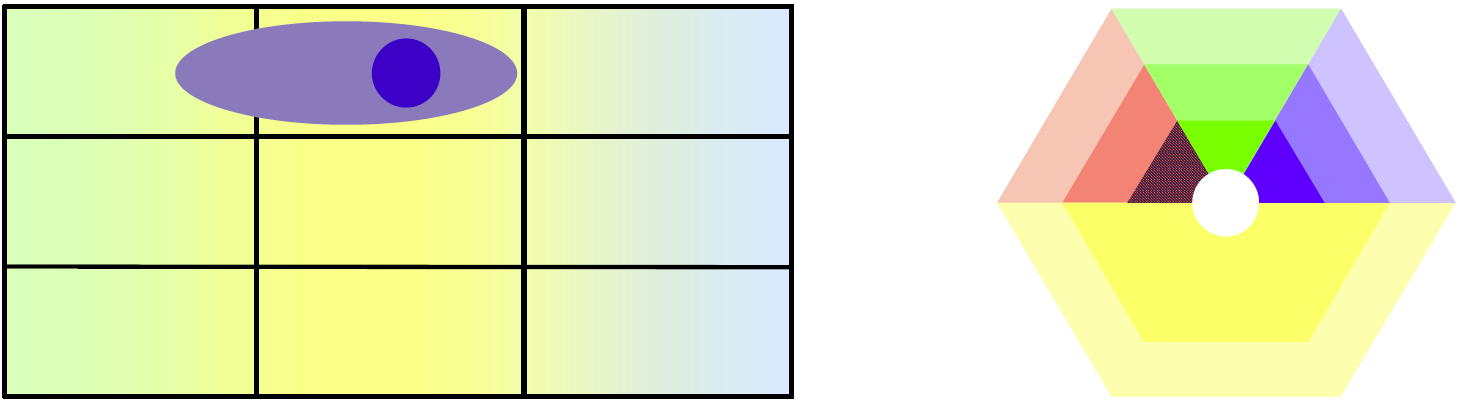
\includegraphics[scale=0.2]{figuras/17}
  	\captionsetup{width=.95\textwidth}
  	\caption{Posición del punto de vista proceso de negocio conceptualmente y marco del punto de vista \cite{ref9}}
  	\label{figura17}
  \end{figure}
  
  \subsection{Metamodelo\index{Metamodelo}}
  La Figura \ref{metamodelo4} se aprecia que el proceso de negocio tiene que ver con un rol o conjunto de roles, el proceso de negocio es disparado por un evento y el proceso de negocio genera un evento o un proceso de eventos, los procesos no son máquinas infinitas todo proceso es
  iniciado por uno o un conjunto de eventos.
  
  Los procesos generan objetos de negocio que es la representación del trabajo en la organización,  el servicio de negocio es lo que el proceso de negocio lleva a cabo estableciéndose entre los dos una relación de realización, el servicio es el core de negocio lo que el cliente mira, el proceso de negocio es lo que implementa realiza, materializa el servicio y el proceso de negocio funciona porque existen unos roles que se encargan de realizar el proceso. \cite{ref9}
  
  \begin{figure}[H]
  	\centering
  	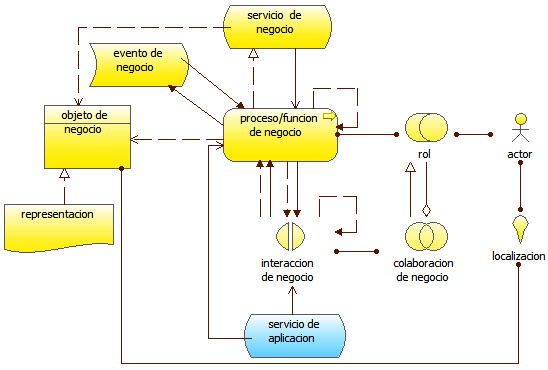
\includegraphics{metamodelos/4}
  	\captionsetup{width=.95\textwidth}
  	\caption{Metamodelo\index{Metamodelo} Punto de Vista Proceso\index{Proceso} de Negocio\index{Negocio} \cite{ref9}}
  	\label{metamodelo4}
  \end{figure}
  
  \subsection{Modelo mInstituto}
  En esta vista se evidencian los procesos que se deben alinear para obtener un producto con un mayor valor agregado, para Creatics, se identifican los procesos de recepción de solicitud, firma del contrato, recepción y/o confirmación del pago y por último la generación de la licencia de uso y acceso a la plataforma.
  
  \begin{figure}[H]
  	\centering
  	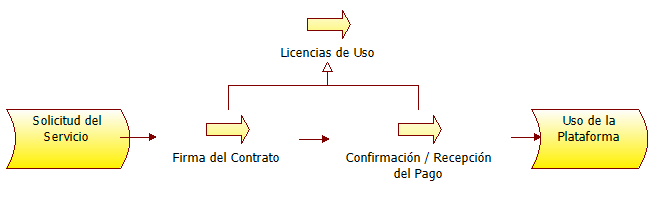
\includegraphics[scale=0.7]{modelos/4}
  	\captionsetup{width=.95\textwidth}
  	\caption{Modelo Punto de Vista Proceso\index{Proceso} de Negocio\index{Negocio}: minstituto}
  	\label{modelo4}
  \end{figure}
  
  %aquí
  \section{Punto de Vista Cooperación\index{Cooperación} de Proceso\index{Proceso} de Negocio\index{Negocio}}
  El punto de vista de cooperación de proceso de negocio es usado para mostrar las relaciones
  de uno o mas procesos de negocio con los demás procesos de negocio y / o con su ambiente. Puede ser usado tanto para crear un diseño de alto nivel de procesos de negocio dentro de su contexto como para proveer un responsable administrador operacional para uno o mas de tales procesos con mando en sus dependencias. \cite{ref9}
  
  \begin{table}[H]
  	\centering
  	\begin{tabular}{p{3.7cm}p{8cm}}
  		\hline
  		\rowcolor[HTML]{0073a1}
  		{\color[HTML]{FFFFFF} \textbf{Nombre}} & {\color[HTML]{FFFFFF} \textbf{Cooperación\index{Cooperación} de Proceso\index{Proceso} de Negocio\index{Negocio}}} \\
  		\hline
  		\textbf{Stakeholder\index{Stakeholder}s} & Proceso\index{Proceso}s, Arquitectos de domino, Gerentes de Operaciones \\
  		\textbf{Preocupaciones} & Dependencias de los procesos de negocio, Responsabilidades \\
  		\textbf{Propósito} & Diseñar\index{Diseñar}, decidir \\
  		\textbf{Nivel de Abstracción\index{Abstracción}} & Coherencia\index{Coherencia} \\
  		\textbf{Capa} & Capa de Negocio\index{Negocio} (Aplicación\index{Aplicación}) \\
  		\textbf{Aspectos} & Comportamiento\index{Comportamiento}, (activo), (pasivo) \\
  		\bottomrule
  	\end{tabular}
  	\captionsetup{width=.95\textwidth}
  	\caption{Descripción punto de vista de cooperación de proceso \cite{ref9}}
  	\label{tabla8}
  \end{table}
  
  \begin{figure}[H]
  	\centering
  	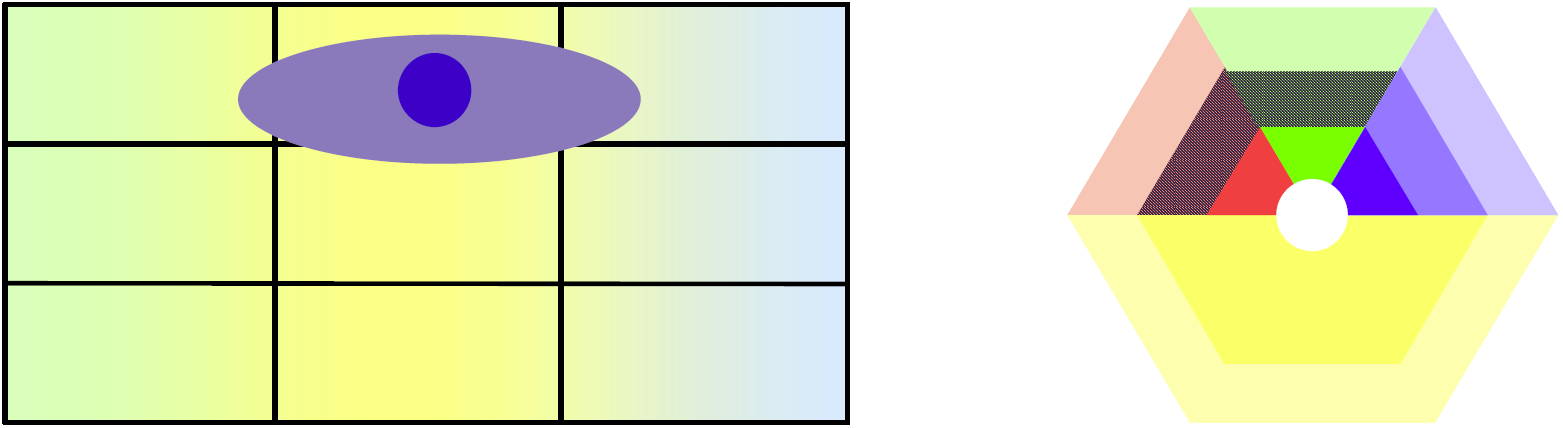
\includegraphics[scale=0.2]{figuras/18}
  	\captionsetup{width=.95\textwidth}
  	\caption{Posición del punto de vista de cooperación de proceso conceptualmente y marco del punto de vista \cite{ref9}}
  	\label{figura18}
  \end{figure}
  
  \subsection{Metamodelo\index{Metamodelo}}
  En la Figura \ref{metamodelo5} se ilustra el metamodelo perteneciente al punto de vista de cooperación de proceso el cual esta compuesto de los conceptos de los procesos del negocio y sus responsabilidades. En este punto de vista a al proceso se le asigna un rol, el rol se compone de interfaces, a la interface se le asigna interacciones y estas interacciones van a una capa de aplicación a través de una interface. \cite{ref9}
  
  \begin{figure}[H]
  	\centering
  	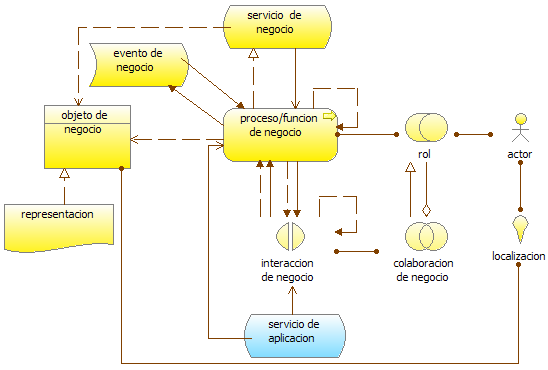
\includegraphics{metamodelos/5}
  	\captionsetup{width=.95\textwidth}
  	\caption{Metamodelo\index{Metamodelo} Punto de Vista de Producto\index{Producto} \cite{ref9}}
  	\label{metamodelo5}
  \end{figure}
  
  \subsection{Modelo mInstituto}
  En la vista se describe el soporte y razón de ser de Minstituto\index{Minstituto}.com que es generar soluciones tecnológicas aplicadas a la administración educativa, convirtiéndose en el objetivo estratégico de la organización. \\
  
  La plataforma web que corresponde a la ubicación del producto, es el medio que proporciona al cliente la confidencialidad, integridad y disponibilidad que su información y funciones de negocio necesitan. \\
  
  El acceso a la plataforma se establece a través de la generación de la licencia y en el contrato se determinan las diferentes características del producto, incluyendo actualizaciones y soporte especializado.
  
  \begin{figure}[H]
  	\centering
  	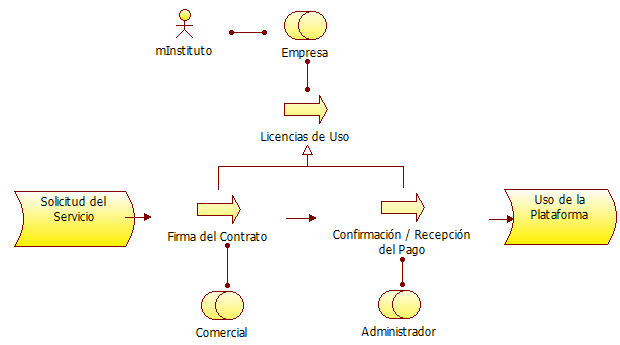
\includegraphics[scale=0.7]{modelos/5}
  	\captionsetup{width=.95\textwidth}
  	\caption{Modelo Punto de Vista de Producto\index{Producto}: minstituto}
  	\label{modelo5}
  \end{figure}
  
\section{Punto de Vista de Producto\index{Producto}}
Este punto de vista se describe como eje central el valor que uno o más productos ofrecen a la clientes u otras partes externas involucradas con la organización, muestra además la composición de uno o más productos en términos de cómo están compuestos, la asociación, el contrato y otros acuerdos. El punto de vista del producto se suele utilizar en el desarrollo de productos para diseñar un producto componiendo servicios existentes o mediante la identificación de nuevos servicios que se tienen que crear para este producto, dado el valor que un cliente espera de ella. \cite{ref9}

  \begin{table}[H]
  	\centering
  	\begin{tabular}{p{3.7cm}p{8cm}}
  		\hline
  		\rowcolor[HTML]{0073a1}
  		{\color[HTML]{FFFFFF} \textbf{Nombre}} & {\color[HTML]{FFFFFF} \textbf{Vista de Producto\index{Producto}}} \\
  		\hline
  		\textbf{Stakeholder\index{Stakeholder}s} & Diseñadores de producto, gerentes de producto, Arquitectos de proceso y de dominio \\
  		\textbf{Preocupaciones} & Desarrollo\index{Desarrollo} del producto y el valor que este ofrece a la organización \\
  		\textbf{Propósito} & Diseñar\index{Diseñar}, decidir \\
  		\textbf{Nivel de Abstracción\index{Abstracción}} & Coherencia\index{Coherencia} \\
  		\textbf{Capa} & Capa de Negocio\index{Negocio} (Aplicación\index{Aplicación}) \\
  		\textbf{Aspectos} & Comportamiento\index{Comportamiento}, información, (activo) \\
  		\bottomrule
  	\end{tabular}
	\captionsetup{width=.95\textwidth}
	\caption{Descripción Punto de Vista de Producto\index{Producto} \cite{ref9}}
	\label{tabla9}
  \end{table}

  \begin{figure}[H]
	\centering
	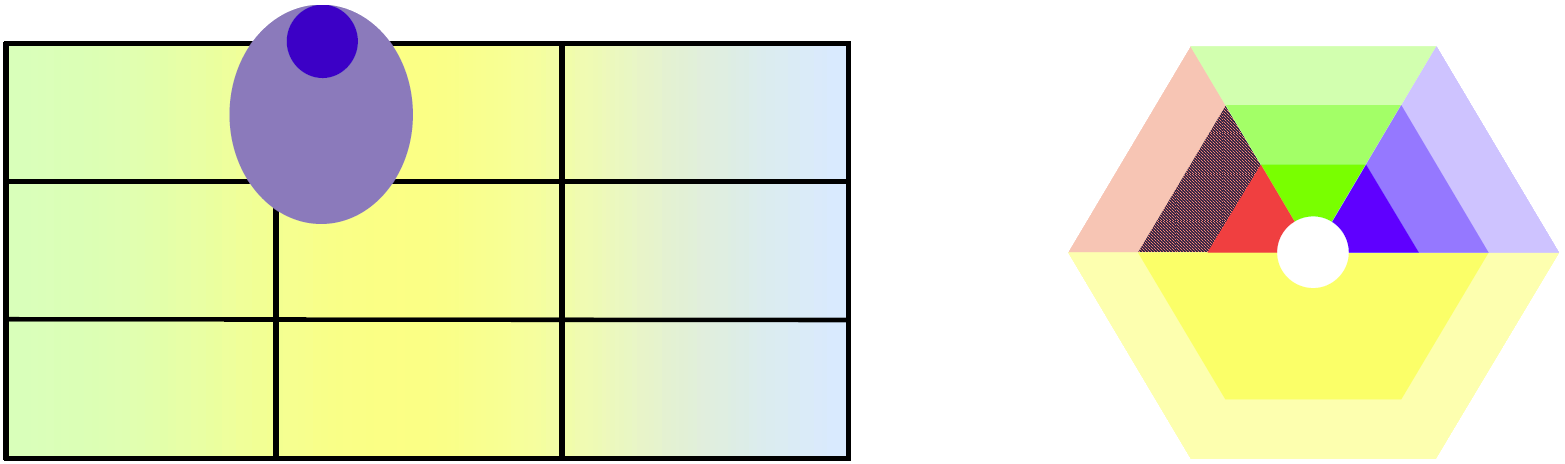
\includegraphics[scale=0.2]{figuras/19}
	\captionsetup{width=.95\textwidth}
	\caption{Posición del Punto de Vista de Producto\index{Producto} conceptualmente y marco del punto de vista \cite{ref9}}
	\label{figura19}
  \end{figure}
  
  \subsection{Metamodelo\index{Metamodelo}}
  La Figura \ref{metamodelo6} ilustra el punto de vista de producto el cual es la convergencia de los puntos de vista anteriores, es el esfuerzo por conocer la estructura, el esfuerzo por saber qué hace cada persona todo converge en el punto de vista que apunta al producto, el cual es un conjunto de servicios al cual se le adhiere un contrato y como elemento clave se le destaca un valor; el producto reposa sobre los procesos que son hechos por unos roles de negocio los cuales corresponden a unos actores. \cite{ref9}

  \begin{figure}[H]
	\centering
	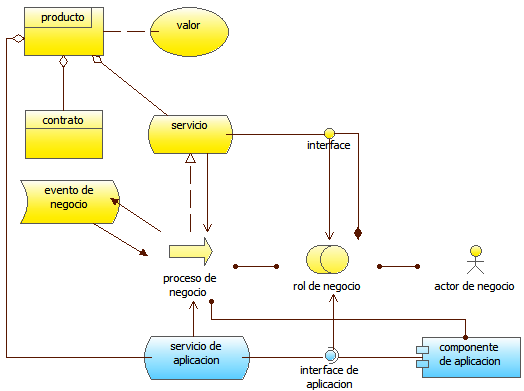
\includegraphics{metamodelos/6}
	\captionsetup{width=.95\textwidth}
	\caption{Metamodelo\index{Metamodelo} Punto de Vista de Producto\index{Producto} \cite{ref9}}
	\label{metamodelo6}
  \end{figure}

  \subsection{Modelo mInstituto}
  El soporte y razón de ser de Minstituto\index{Minstituto}.com es generar soluciones tecnológicas aplicadas a la administración educativa, siendo la plataforma web el medio que proporciona al cliente la confidencialidad, integridad y disponibilidad que su información y funciones de negocio necesitan.  El acceso a la plataforma se establece a través de la generación de la licencia y en el contrato se determinan las diferentes características del producto, incluyendo actualizaciones y soporte especializado.

  \begin{figure}[H]
	\centering
	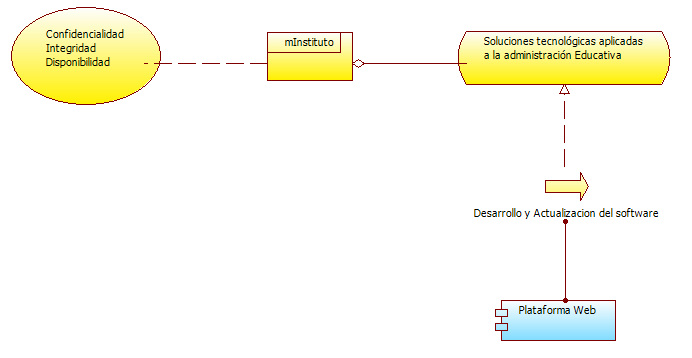
\includegraphics[scale=0.7]{modelos/6}
	\captionsetup{width=.95\textwidth}
	\caption{Modelo Punto de Vista de Producto\index{Producto}: minstituto}
	\label{modelo6}
  \end{figure}
		\chapter{Capa de Aplicación\index{Aplicación}}
\label{chap:Aplicacion}
\textit{El capítulo presenta el desarrollo de la Arquitectura Empresarial\index{Arquitectura Empresarial} correspondiente a la Capa de Aplicación\index{Aplicación} utilizando Archimate\index{Archimate}.}
\vspace{2ex}\vfill
\minitoc
\cleardoublepage

\section{Punto de Vista Comportamiento\index{Comportamiento} de Aplicación\index{Aplicación}}
El punto de vista del comportamiento de aplicaciones describe el comportamiento interno de la aplicación, este punto de vista es útil en el diseño del comportamiento principal de aplicaciones, o en la identificación de solapamiento funcional entre diferentes aplicaciones. \cite{ref9}

  \begin{table}[H]
  	\centering
  	\begin{tabular}{p{3.7cm}p{8cm}}
  		\hline
  		\rowcolor[HTML]{0073a1}
  		{\color[HTML]{FFFFFF} \textbf{Nombre}} & {\color[HTML]{FFFFFF} \textbf{Comportamiento\index{Comportamiento} de Aplicación\index{Aplicación}}} \\
  		\hline
  		\textbf{Stakeholder\index{Stakeholder}s} & Arquitectos de la organización, proceso, aplicación y dominio \\
  		\textbf{Preocupaciones} & Estructura\index{Estructura}r las relaciones entre las aplicaciones, garantizar la consistencia e integridad, reducir la complejidad \\
  		\textbf{Propósito} & Diseñar\index{Diseñar} \\
  		\textbf{Nivel de Abstracción\index{Abstracción}} & Coherencia\index{Coherencia}, detalle \\
  		\textbf{Capa} & Capa de Aplicación\index{Aplicación} (Aplicación\index{Aplicación}) \\
  		\textbf{Aspectos} & Activo, comportamiento, (información) \\
  		\bottomrule
  	\end{tabular}
	\captionsetup{width=.95\textwidth}
	\caption{Descripción punto de vista comportamiento de aplicación \cite{ref9}}
	\label{tabla10}
  \end{table}

  \begin{figure}[H]
	\centering
	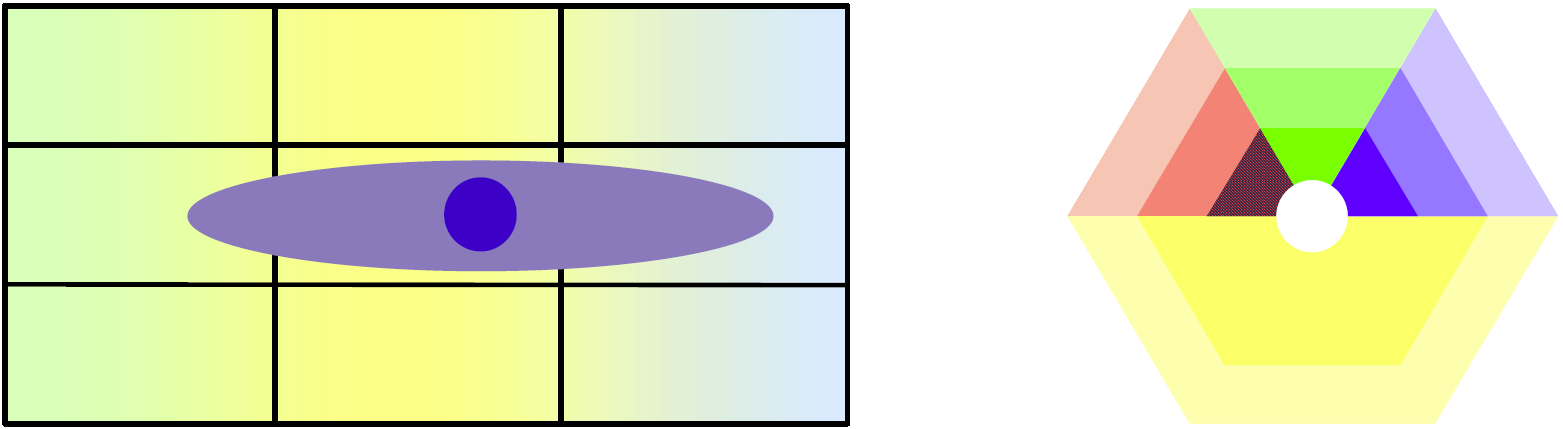
\includegraphics[scale=0.2]{figuras/20}
	\captionsetup{width=.95\textwidth}
	\caption{Posición del punto de vista comportamiento de aplicación conceptualmente y marco del punto de vista \cite{ref9}}
	\label{figura20}
  \end{figure}

\subsection{Metamodelo\index{Metamodelo}}
En la Figura \ref{metamodelo7} se ilustra el metamodelo perteneciente al punto de vista comportamiento de aplicación, el concepto clave para la estructura es el componente de aplicación, a este componentes se le asignan funciones de aplicación, las cuales realizan los servicios de aplicación donde estos servicios soportan los procesos de negocio, se generan unos objetos de datos; la interface es la encargada de interconectar los componentes, en el metamodelo aparece la colaboración de aplicación donde se reúnen componentes que aplican el concepto de colaboración. \cite{ref9}

\begin{figure}[H]
	\centering
	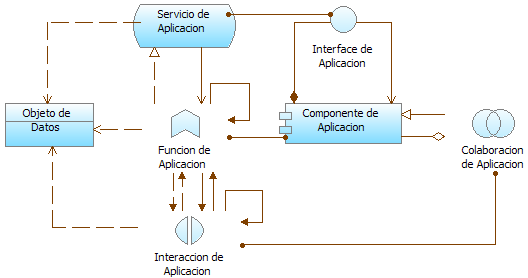
\includegraphics{metamodelos/7}
	\captionsetup{width=.95\textwidth}
	\caption{Metamodelo\index{Metamodelo} punto de vista comportamiento de aplicación \cite{ref9}}
	\label{metamodelo7}
\end{figure}

  \subsection{Modelo mInstituto}
  En el punto de vista se describe la funcionalidad de cada componente de aplicación, se encuentran los siguientes componentes y su funcionalidad; el licenciamiento tiene como funcionalidad permitir el acceso de los perfiles y usuarios configurados, garantizar transacciones seguras y generar los respectivos soportes contables de las transacciones. \\
  
  El producto tiene como funcionalidad brindar la información necesaria en cuanto a las características del mismo y condiciones de adquisición, además incluye las respectivas actualizaciones del sistema. La comunidad tiene como funcionalidad proveer de herramientas de comunicación entre grupos de estudiantes así como enlazar la comunicación con las redes sociales. \\
  
  Por último la el componente de publicidad tiene como funcionalidad ampliar la participación en el mercado a través de las estrategias de marketing que se utilicen.

\begin{figure}[H]
	\centering
	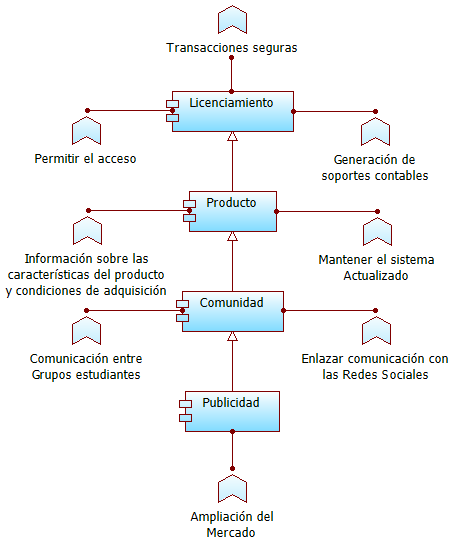
\includegraphics[scale=0.7]{modelos/7}
	\captionsetup{width=.95\textwidth}
	\caption{Modelo punto de vista comportamiento de aplicación: minstituto}
	\label{modelo7}
\end{figure}

\section{Punto de Vista Cooperación\index{Cooperación} de Aplicación\index{Aplicación}}
El punto de vista de Cooperación\index{Cooperación} de la aplicación describe las relaciones entre los componentes de las aplicaciones en función de los flujos de información entre ellos, o en términos de los servicios que ofrecen y su uso. \\

Este punto de vista también se utiliza para expresar la cooperación (interna) o la orquestación de los servicios que en conjunto apoyan la ejecución de un proceso de negocio. \cite{ref9}

  \begin{table}[H]
  	\centering
  	\begin{tabular}{p{3.7cm}p{8cm}}
  		\hline
  		\rowcolor[HTML]{0073a1}
  		{\color[HTML]{FFFFFF} \textbf{Nombre}} & {\color[HTML]{FFFFFF} \textbf{Cooperación\index{Cooperación} de Aplicación\index{Aplicación}}} \\
  		\hline
  		\textbf{Stakeholder\index{Stakeholder}s} & Arquitectos de la organización, proceso, aplicación y dominio \\
  		\textbf{Preocupaciones} & Estructura\index{Estructura}r las relaciones y dependencias entre las aplicaciones, orquestación de los servicios, garantizar la consistencia e integridad, reducir la complejidad \\
  		\textbf{Propósito} & Diseñar\index{Diseñar} \\
  		\textbf{Nivel de Abstracción\index{Abstracción}} & Coherencia\index{Coherencia}, detalle \\
  		\textbf{Capa} & Capa de Aplicación\index{Aplicación} (Aplicación\index{Aplicación}) \\
  		\textbf{Aspectos} & Activo, comportamiento \\
  		\bottomrule
  	\end{tabular}
  	\captionsetup{width=.95\textwidth}
  	\caption{Descripción punto de vista cooperación de aplicación \cite{ref9}}
  	\label{tabla11}
  \end{table}

\begin{figure}[H]
	\centering
	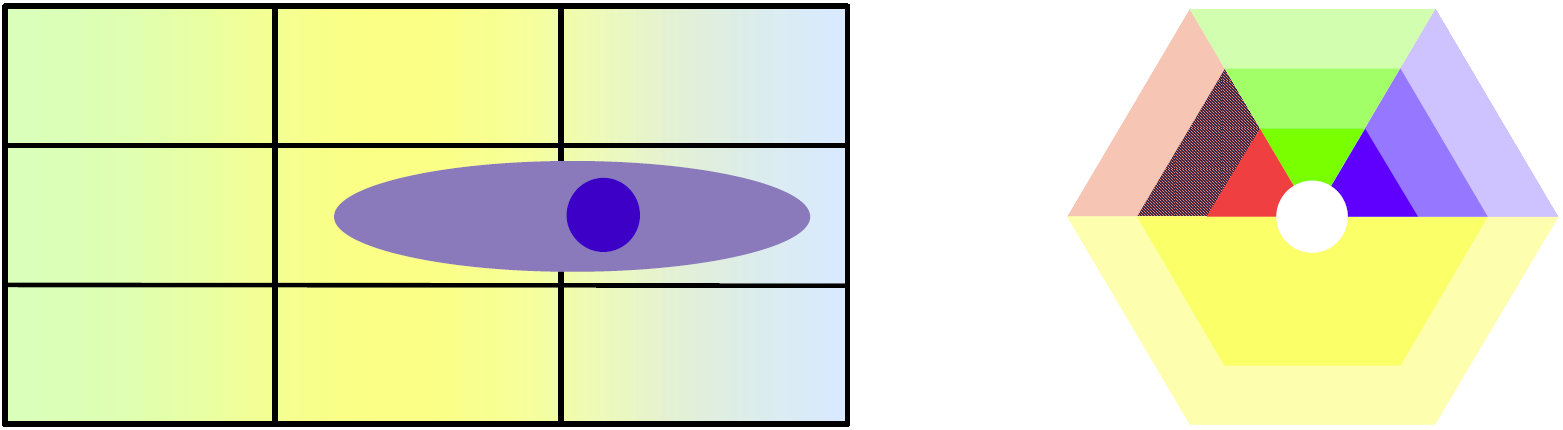
\includegraphics[scale=0.2]{figuras/21}
	\captionsetup{width=.95\textwidth}
	\caption{Posición del punto de vista cooperación de aplicación conceptualmente y marco del punto de vista \cite{ref9}}
	\label{figura21}
\end{figure}

\subsection{Metamodelo\index{Metamodelo}}
En la figura Figura \ref{metamodelo8} se ilustra el metamodelo perteneciente al punto de vista cooperación de aplicación, el punto de vista se centra en la localización,ya que se agrupan los componentes en un front office y un back office. \cite{ref9}

\begin{figure}[H]
	\centering
	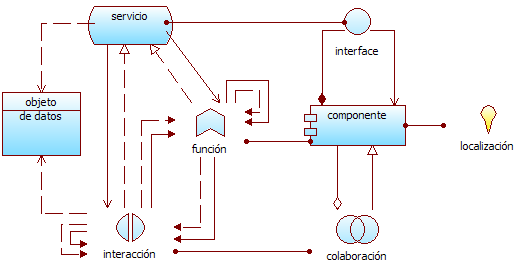
\includegraphics{metamodelos/8}
	\captionsetup{width=.95\textwidth}
	\caption{Metamodelo\index{Metamodelo} punto de vista cooperación de aplicación \cite{ref9}}
	\label{metamodelo8}
\end{figure}

\subsection{Modelo mInstituto}
En el punto de vista se evidencia que la localización del front office se encuentran los componentes de publicidad, minstituto y comunidad, por otro lado en la localización del back office se encuentran ubicados los componentes de diseño, análisis y desarrollo los cuales se relacionan directamente con la aplicación Minstituto\index{Minstituto}.

\begin{figure}[H]
	\centering
	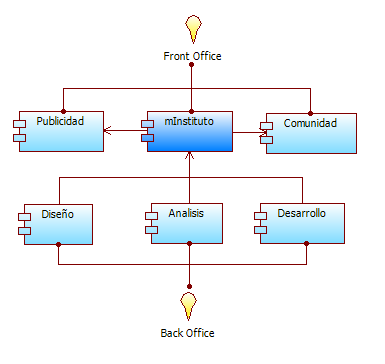
\includegraphics[scale=0.7]{modelos/8}
	\captionsetup{width=.95\textwidth}
	\caption{Modelo Punto de Vista Cooperación\index{Cooperación} de Aplicación\index{Aplicación}: minstituto}
	\label{modelo8}
\end{figure}

\section{Punto de Vista Estructura\index{Estructura} de Aplicación\index{Aplicación}}
El punto de vista de estructura de la aplicación, muestra la estructura de componentes de una aplicación Este punto de vista es útil en el diseño o la comprensión de la estructura principal de componentes de la aplicación y el uso de datos asociados. \cite{ref9}

  \begin{table}[H]
  	\centering
  	\begin{tabular}{p{3.7cm}p{8cm}}
  		\hline
  		\rowcolor[HTML]{0073a1}
  		{\color[HTML]{FFFFFF} \textbf{Nombre}} & {\color[HTML]{FFFFFF} \textbf{Estructura\index{Estructura} de Aplicación\index{Aplicación}}} \\
  		\hline
  		\textbf{Stakeholder\index{Stakeholder}s} & Arquitectos de la organización, aplicación y dominio \\
  		\textbf{Preocupaciones} & Estructura\index{Estructura} de la aplicación, garantizar la consistencia e integridad, reducir la complejidad \\
  		\textbf{Propósito} & Diseñar\index{Diseñar} \\
  		\textbf{Nivel de Abstracción\index{Abstracción}} & Detalle \\
  		\textbf{Capa} & Capa de Aplicación\index{Aplicación} \\
  		\textbf{Aspectos} & Activo, (Pasivo) \\
  		\bottomrule
  	\end{tabular}
  	\captionsetup{width=.95\textwidth}
  	\caption{Descripción punto de vista estructura de aplicación \cite{ref9}}
  	\label{tabla12}
  \end{table}

  \begin{figure}[H]
	\centering
	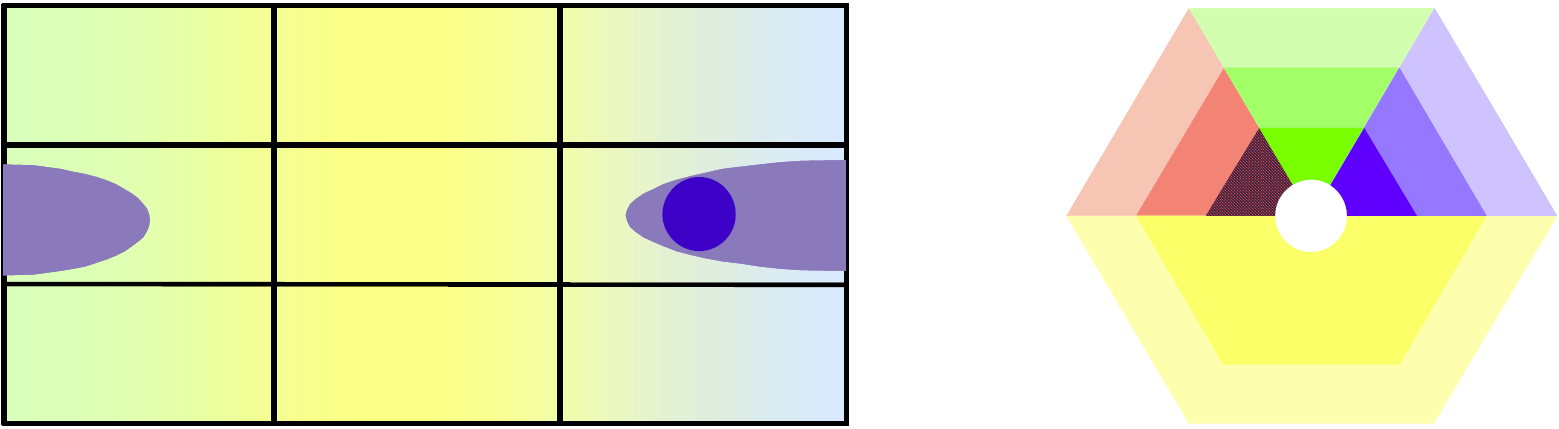
\includegraphics[scale=0.2]{figuras/22}
	\captionsetup{width=.95\textwidth}
	\caption{Posición del punto de vista estructura de aplicación conceptualmente y marco del punto de vista \cite{ref9}}
	\label{figura22}
  \end{figure}

  \subsection{Metamodelo\index{Metamodelo}}
  En la figura Figura \ref{metamodelo9} se ilustra el metamodelo perteneciente al punto de vista de estructura de la aplicación en este metamodelo se involucran el componente y la interfaz, se muestra la forma de interactuar el sistema con los componentes de software haciendo uso de las interfaces de comunicación.\cite{ref9}

  \begin{figure}[H]
	\centering
	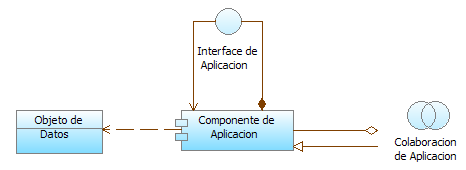
\includegraphics{metamodelos/9}
	\captionsetup{width=.95\textwidth}
	\caption{Metamodelo\index{Metamodelo} punto de vista estructura de aplicación \cite{ref9}}
	\label{metamodelo9}
  \end{figure}

  \subsection{Modelo mInstituto}
  En la vista se describe el mecanismo de comunicación entre los componentes, se define como componente central minstituto siendo el componente más importante en el cumplimiento de la misión de la organización, la comunicación de éste con los demás componentes se genera a través de interfaces.
  
  \begin{figure}[H]
	\centering
	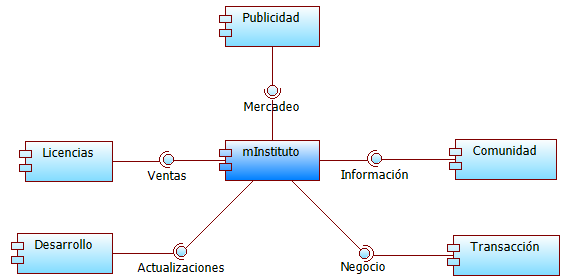
\includegraphics[scale=0.7]{modelos/9}
	\captionsetup{width=.95\textwidth}
	\caption{Modelo punto de vista estructura de aplicación: minstituto}
	\label{modelo9}
  \end{figure}
  
  \section{Punto de Vista de Uso de Aplicación\index{Aplicación}}
  El punto de vista de uso de aplicación describe como las aplicaciones son usadas para soportar uno o mas procesos de negocio, y como ellos son usados por otras aplicaciones. Puede ser usado en el diseño de una aplicación para identificar los servicios requeridos por los procesos de negocios y otras aplicaciones, o en el diseño de procesos de negocio para describir los servicios que están disponibles. Así, al identificar las dependencias de los procesos de negocio sobre las aplicaciones, puede ser útil para los administradores operativos responsables de estos procesos. \cite{ref9}
  
  \begin{table}[H]
  	\centering
  	\begin{tabular}{p{3.7cm}p{8cm}}
  		\hline
  		\rowcolor[HTML]{0073a1}
  		{\color[HTML]{FFFFFF} \textbf{Nombre}} & {\color[HTML]{FFFFFF} \textbf{Uso de Aplicación\index{Aplicación}}} \\
  		\hline
  		\textbf{Stakeholder\index{Stakeholder}s} & La empresa, el proceso, los arquitectos de aplicaciones, directores de operaciones \\
  		\textbf{Preocupaciones} & Consistencia e Integridad\index{Integridad}, Reducción de la complejidad \\
  		\textbf{Propósito} & Diseñar\index{Diseñar}, decidir \\
  		\textbf{Nivel de Abstracción\index{Abstracción}} & Coherencia\index{Coherencia} \\
  		\textbf{Capa} & Capa de Negocio\index{Negocio} y Aplicación\index{Aplicación} \\
  		\textbf{Aspectos} & Comportamiento\index{Comportamiento}, estructura \\
  		\bottomrule
  	\end{tabular}
  	\captionsetup{width=.95\textwidth}
  	\caption{Descripción punto de vista de Uso de Aplicación\index{Aplicación} \cite{ref9}}
  	\label{tabla13}
  \end{table}
  
  \begin{figure}[H]
  	\centering
  	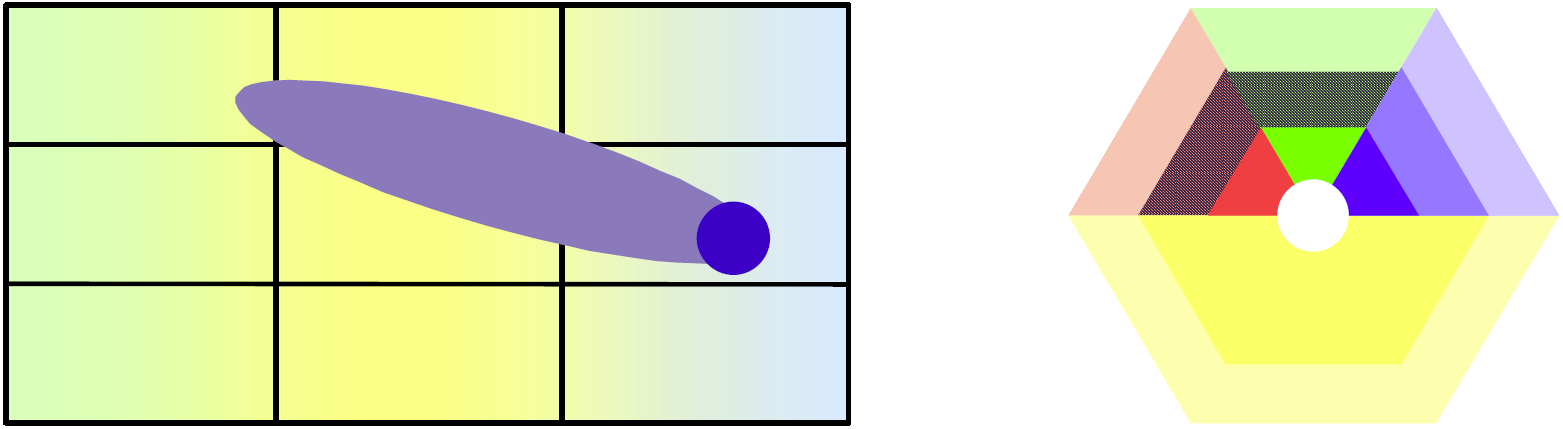
\includegraphics[scale=0.2]{figuras/23}
  	\captionsetup{width=.95\textwidth}
  	\caption{Posición del punto de vista de Uso de Aplicación\index{Aplicación} conceptualmente y marco del punto de vista \cite{ref9}}
  	\label{figura23}
  \end{figure}
  
  \subsection{Metamodelo\index{Metamodelo}}
  En la figura Figura \ref{metamodelo10} se ilustra el metamodelo perteneciente al punto de vista de Uso de Aplicación\index{Aplicación} en este metamodelo se involucran el componente y la interfaz, se muestra la forma de usar el software haciendo uso de las interfaces y componentes. \\
  
  Puede ser usado en el diseño de una aplicación para identificar los servicios requeridos por los procesos de negocios y otras aplicaciones, o en el diseño de procesos de negocio para describir los servicios que están disponibles. Así, al identificar las dependencias de los procesos de negocio sobre las aplicaciones, puede ser útil para los administradores operativos responsables de estos procesos. \cite{ref9}
  
  \begin{figure}[H]
  	\centering
  	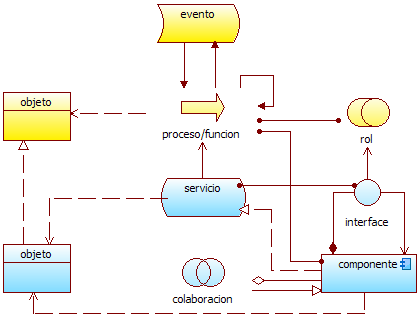
\includegraphics{metamodelos/10}
  	\captionsetup{width=.95\textwidth}
  	\caption{Metamodelo\index{Metamodelo} punto de vista de Uso de Aplicación\index{Aplicación} \cite{ref9}}
  	\label{metamodelo10}
  \end{figure}
  
  \subsection{Modelo mInstituto}
  En la vista se destacan los servicios de aplicación fundamentales para el proceso de negocio, los cuales son el desarrollo de la aplicación y la generación de las licencias. \\
  
  La generación de licencias incluye los servicios de acceso a la aplicación y la realización de los pagos utilizando el componente de transacciones. Por otro lado el desarrollo de aplicación incluye las mejoras y actualizaciones utilizando el componente de desarrollo.\\
  
  Los dos procesos generados en la capa de aplicación están directamente relacionados con el cliente y pertenecen a los procesos misionales. Por una parte el cliente obtiene el acceso al software y por el otro a las actualizaciones del mismo.
  
  \begin{figure}[H]
  	\centering
  	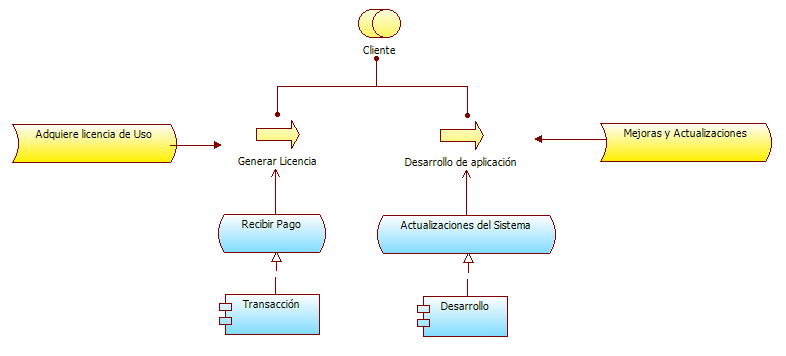
\includegraphics[scale=0.7]{modelos/10}
  	\captionsetup{width=.95\textwidth}
  	\caption{Modelo punto de vista de Uso de Aplicación\index{Aplicación}: minstituto}
  	\label{modelo10}
  \end{figure}
		\chapter{Capa de Infraestructura\index{Infraestructura}}
\label{chap:Infraestructura}
\textit{El siguiente capítulo representa el desarrollo de la Arquitectura Empresarial\index{Arquitectura Empresarial} correspondiente a la Capa de Infraestructura\index{Infraestructura} utilizando Archimate\index{Archimate}.}
\vspace{2ex}\vfill
\minitoc
\newpage

\section{Punto de Vista de Infraestructura\index{Infraestructura}}
El punto de vista de infraestructura contiene los elementos de la infraestructura de cómputo y hardware de comunicación de apoyo a la capa de aplicación, tales como dispositivos o redes físicas.La Tabla \ref{tabla14} describe el punto de vista. \cite{ref9}

  \begin{table}[H]
  	\centering
  	\begin{tabular}{p{3.7cm}p{8cm}}
  		\hline
  		\rowcolor[HTML]{0073a1}
  		{\color[HTML]{FFFFFF} \textbf{Nombre}} & {\color[HTML]{FFFFFF} \textbf{Vista de Infraestructura\index{Infraestructura}}} \\
  		\hline
  		\textbf{Stakeholder\index{Stakeholder}s} & Arquitectos de infraestructura y aplicación gerentes de operación \\
  		\textbf{Preocupaciones} & Dependencias, escalabilidad y performance  \\
  		\textbf{Propósito} & Diseñar\index{Diseñar} \\
  		\textbf{Nivel de Abstracción\index{Abstracción}} & Coherencia\index{Coherencia} \\
  		\textbf{Capa} & Capa de Tecnología\index{Tecnología} \\
  		\textbf{Aspectos} & Comportamiento\index{Comportamiento}, activa \\
  		\bottomrule
  	\end{tabular}
  	\captionsetup{width=.95\textwidth}
  	\caption{Descripción punto de vista de Infraestructura\index{Infraestructura} \cite{ref9}}
  	\label{tabla14}
  \end{table}

  \begin{figure}[H]
	\centering
	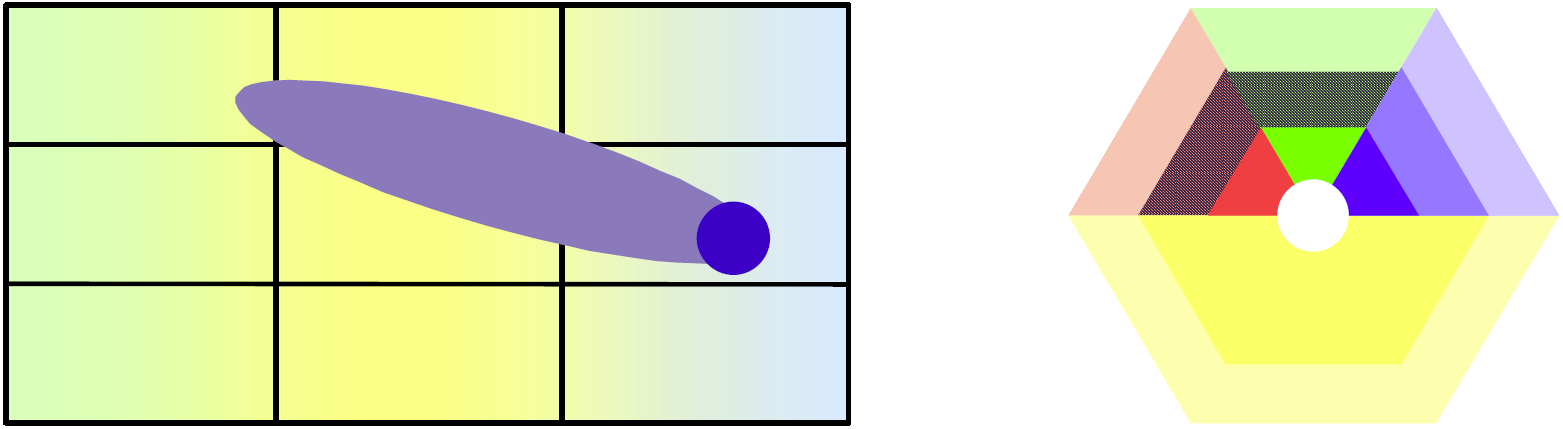
\includegraphics[scale=0.2]{figuras/23}
	\captionsetup{width=.95\textwidth}
	\caption{Posición del punto de vista de infraestructura conceptual y marco del punto de vista \cite{ref9}}
	\label{figura23a}
  \end{figure}

  \subsection{Metamodelo\index{Metamodelo}}
  El metamodelo de la Figura \ref{metamodelo11} se centra en los nodos y los componentes, se muestra como las piezas de software están contenidas en los recursos físicos.\cite{ref9}

  \begin{figure}[H]
	\centering
	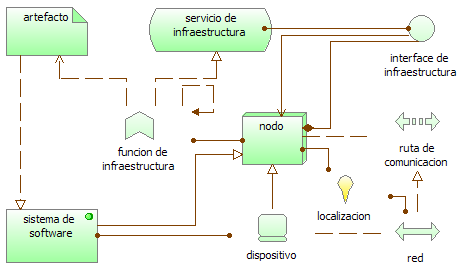
\includegraphics{metamodelos/11}
	\captionsetup{width=.95\textwidth}
	\caption{Metamodelo\index{Metamodelo} punto de vista de infraestructura \cite{ref9}}
	\label{metamodelo11}
  \end{figure}

  \subsection{Modelo mInstituto}
  La infraestructura para el aplicativo mInstituto esta basada en un portal comercial el cual se ejecuta sobre un servidor de páginas web y necesitara de un hosting que cumpla las restricciones de costos y a su vez lleve la menor cantidad de soporte a nivel de seguridad ya que la funcionalidad principal es la de ofrecer información sobre los productos de la organización y realizar actualizaciones que no van mas allá de noticias relacionadas con la empresa, producto o el medio en el que nos desenvolvemos. \\
  
  Por otro lado tenemos nuestro portal para el aplicativo, este estará hospedado en un proveedor de servicios que responda con las necesidades de base de datos así como la demanda de consulta de todos los módulos.  \\
  
  La comunicación se realizará a través del proveedor de servicios de Internet\index{Internet} contratado por el cliente, utilizando la red y equipos de propiedad del cliente en su respectiva localización. \\
  
  \begin{figure}[H]
	\centering
	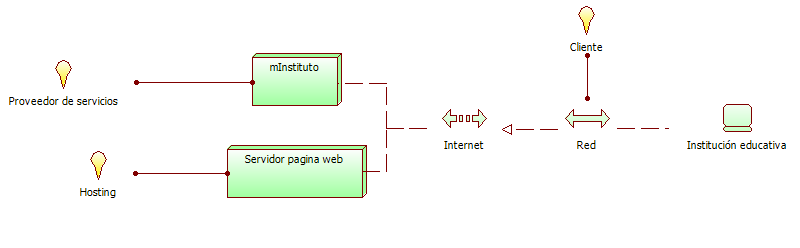
\includegraphics[scale=0.7]{modelos/11}
 	\captionsetup{width=.95\textwidth}
	\caption{Modelo punto de vista de infraestructura: minstituto}
	\label{modelo11}
  \end{figure}
  
  \section{Punto de Vista Uso de Infraestructura\index{Infraestructura}}
  El punto de vista de uso Infraestructura\index{Infraestructura} muestra cómo las aplicaciones son compatibles con el software y hardware de infraestructura: los servicios de infraestructura son entregados por los dispositivos; el software y redes de sistema se proporcionan a las aplicaciones. Este punto de vista desempeña un papel importante en el análisis de rendimiento y escalabilidad, puesto que se refiere la infraestructura física para el mundo lógico de aplicaciones. Es muy útil en la determinación de los requisitos de rendimiento y calidad en la infraestructura basada en las exigencias de las diferentes aplicaciones que lo utilizan. \cite{ref9}
  
  \begin{table}[H]
  	\centering
  	\begin{tabular}{p{3.7cm}p{8cm}}
  		\hline
  		\rowcolor[HTML]{0073a1}
  		{\color[HTML]{FFFFFF} \textbf{Nombre}} & {\color[HTML]{FFFFFF} \textbf{Uso de Infraestructura\index{Infraestructura}}} \\
  		\hline
  		\textbf{Stakeholder\index{Stakeholder}s} & Arquitectos de infraestructura y aplicación, gerentes de operación \\
  		\textbf{Preocupaciones} & Dependencias, escalabilidad y rendimiento \\
  		\textbf{Propósito} & Diseñar\index{Diseñar} \\
  		\textbf{Nivel de Abstracción\index{Abstracción}} & Coherencia\index{Coherencia} \\
  		\textbf{Capa} & Capa de Aplicación\index{Aplicación} y Tecnología\index{Tecnología} \\
  		\textbf{Aspectos} & Activo, (comportamiento) \\
  		\bottomrule
  	\end{tabular}
  	\captionsetup{width=.95\textwidth}
  	\caption{Descripción punto de vista uso de infraestructura \cite{ref9}}
  	\label{tabla15}
  \end{table}
  
  \begin{figure}[H]
  	\centering
  	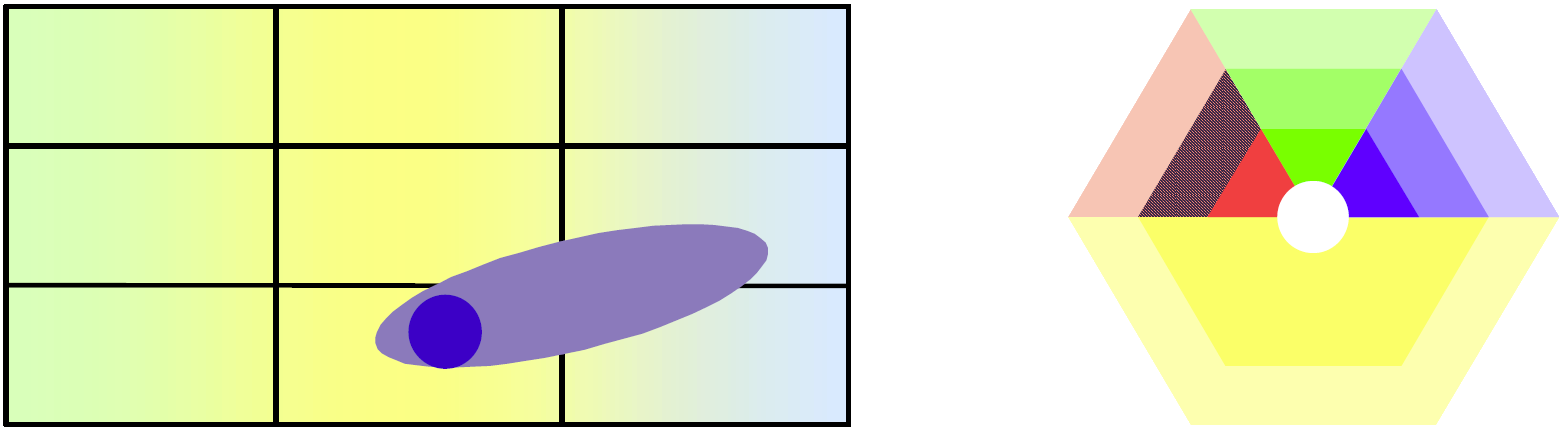
\includegraphics[scale=0.2]{figuras/24}
  	\captionsetup{width=.95\textwidth}
  	\caption{Posición del punto de vista uso de infraestructura conceptualmente y marco del punto de vista \cite{ref9}}
  	\label{figura24}
  \end{figure}
  
  \subsection{Metamodelo\index{Metamodelo}}
  El metamodelo de la Figura \ref{metamodelo12} se centra en los nodos y los componentes, se muestra como las piezas de software están contenidas en los recursos físicos. \cite{ref9}
  
  \begin{figure}[H]
  	\centering
  	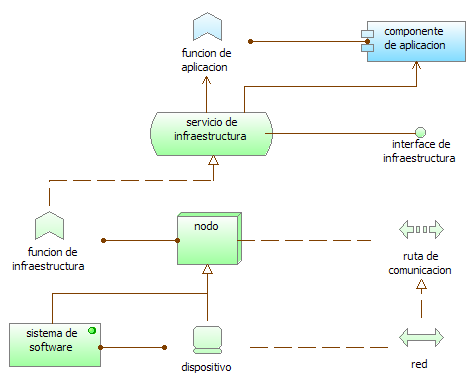
\includegraphics{metamodelos/12}
  	\captionsetup{width=.95\textwidth}
  	\caption{Metamodelo\index{Metamodelo} punto de vista uso de infraestructura \cite{ref9}}
  	\label{metamodelo12}
  \end{figure}
  
  \subsection{Modelo mInstituto}
  El servidor de la página web está destinado a la parte comercial de la empresa, tiene como principales componentes la administración de parte de las estrategias de mercadeo y publicidad y por otro lado se encuentra el acceso a una comunidad basada en redes sociales; este a su vez se comunica con el servidor de aplicaciones a través del punto de acceso o pantalla de login donde nuestros clientes accederán a la aplicación de Minstituto\index{Minstituto}.com, el aplicativo posee herramientas de accesibilidad para los usuarios y perfiles autorizados y tiene incluido un módulo de transacciones y pagos el cual cuenta con el nivel de seguridad informática acorde a las necesidades de la información
  
  \begin{figure}[H]
  	\centering
  	\includegraphics[scale=0.7]{modelos/12}
  	\captionsetup{width=.95\textwidth}
  	\caption{Modelo punto de vista uso de infraestructura: minstituto}
  	\label{modelo12}
  \end{figure}
  
  \section{Punto de Vista de Organización\index{Organización} e Implementación\index{Implementación}}
  La aplicación y el punto de vista de implementación muestran cómo una o más aplicaciones se realizan o se colaboran dentro de la infraestructura, como las aplicaciones son soportadas por el software y el hardware de infraestructura, los servicios de infraestructura son entregados por los dispositivos; el software y las redes del sistema se proporcionan a las aplicaciones, este punto de vista desempeña un papel importante en el análisis de rendimiento y escalabilidad y que hacer referencia a la infraestructura física para el mundo lógico. \cite{ref9}
  
  \begin{table}[H]
  	\centering
  	\begin{tabular}{p{3.7cm}p{8cm}}
  		\hline
  		\rowcolor[HTML]{0073a1}
  		{\color[HTML]{FFFFFF} \textbf{Nombre}} & {\color[HTML]{FFFFFF} \textbf{Organización\index{Organización} e Implementación\index{Implementación}}} \\
  		\hline
  		\textbf{Stakeholder\index{Stakeholder}s} & Arquitectos de infraestructura y aplicación gerente de operación \\
  		\textbf{Preocupaciones} & Dependencias, seguridad, riesgos \\
  		\textbf{Propósito} & Diseñar\index{Diseñar} \\
  		\textbf{Nivel de Abstracción\index{Abstracción}} & Coherencia\index{Coherencia} \\
  		\textbf{Capa} & Capa de tecnología, capa de aplicación \\
  		\textbf{Aspectos} & Activo (Comportamiento\index{Comportamiento}) \\
  		\bottomrule
  	\end{tabular}
  	\captionsetup{width=.95\textwidth}
  	\caption{Descripción punto de vista de organización e implementación \cite{ref9}}
  	\label{tabla16}
  \end{table}
  
  \begin{figure}[H]
  	\centering
  	\includegraphics[scale=0.2]{figuras/25}
  	\captionsetup{width=.95\textwidth}
  	\caption{Posición de la organización e implementación conceptualmente y marco del punto de vista \cite{ref9}}
  	\label{figura25}
  \end{figure}
  
  \subsection{Metamodelo\index{Metamodelo}}
  En el metamodelo de la Figura \ref{metamodelo13} se aprecia como los diferentes nodos de infraestructura que contienen los componentes de aplicación soportan las comunicación entre ellos, muestran como componen elementos de colaboración los cuales permiten tener sistemas de cruce entre sistemas y componentes de aplicación. En el metamodelo se aumenta un componente de infraestructura para reflejar el concepto de colaboración. \\
  
  Visto de otro modo comprende la asignación de aplicaciones y componentes en artefactos y el mapeo de la información utilizada por estas aplicaciones y componentes en la infraestructura de almacenamiento, en pocas palabras establece las relaciones de la infraestructura física con el mundo lógico de las aplicaciones. \cite{ref9}
  
  \begin{figure}[H]
  	\centering
  	\includegraphics{metamodelos/13}
  	\captionsetup{width=.95\textwidth}
  	\caption{Metamodelo\index{Metamodelo} punto de vista de organización e implementación \cite{ref9}}
  	\label{metamodelo13}
  \end{figure}
  
  \subsection{Modelo mInstituto}
  En este punto de vista observamos que Minstituto\index{Minstituto}.com utiliza un servidor Linux\index{Linux} y sobre este se ejecuta el código Java utilizando su máquina virtual y conectado a una base de datos postgreSQL. \\
  
  Para el portal comercial tendremos en un hosting compartido, una página web elaborada en PHP\index{PHP} con una base de datos MySQL\index{MySQL}. Las dos podrán ser consultadas por los clientes usando Internet\index{Internet} de sus proveedor de servicios y un navegador que soporte lenguaje HTML en su última versión, así como tener habilitado la ejecución de código javascript para validaciones necesarias en ambos portales.

  \begin{figure}[H]
  	\centering
  	\includegraphics[scale=0.7]{modelos/13}
  	\captionsetup{width=.95\textwidth}
  	\caption{Modelo punto de vista de organización e implementación: minstituto}
  	\label{modelo13}
  \end{figure}

\section{Punto de Vista de Estructura\index{Estructura} de Información}
El punto de vista de estructura de información es comparable a los modelos tradicionales de información creados en el desarrollo de casi cualquier sistema de información. Se muestra la estructura de la información utilizada en la empresa o en un proceso de negocio específico o aplicación, en términos de tipos de datos o las estructuras de clase (orientada a objetos). Además, puede mostrar cómo se representa la información a nivel de empresa (objetos de negocio), a nivel de aplicación en forma de estructuras de datos utilizadas (objetos de datos), y cómo éstos se asignan a la infraestructura subyacente; por ejemplo por medio de un esquema de base de datos (artefacto). \cite{ref9}
    
    \begin{table}[H]
    	\centering
    	\begin{tabular}{p{3.7cm}p{8cm}}
    		\hline
    		\rowcolor[HTML]{0073a1}
    		{\color[HTML]{FFFFFF} \textbf{Nombre}} & {\color[HTML]{FFFFFF} \textbf{Estructura\index{Estructura} de Información}} \\
    		\hline
    		\textbf{Stakeholder\index{Stakeholder}s} & Arquitectos de dominio e información \\
    		\textbf{Preocupaciones} & Estructura\index{Estructura}, dependencias e inconsistencia del uso de los datos y la información  \\
    		\textbf{Propósito} & Diseñar\index{Diseñar} \\
    		\textbf{Nivel de Abstracción\index{Abstracción}} & Detalle \\
    		\textbf{Capa} & Capa de negocio, capa de tecnología, capa de aplicación \\
    		\textbf{Aspectos} & Pasivo \\
    		\bottomrule
    	\end{tabular}
    	\captionsetup{width=.95\textwidth}
    	\caption{Descripción punto de vista de estructura de información \cite{ref9}}
    	\label{tabla17}
    \end{table}
    
    \begin{figure}[H]
    	\centering
    	\includegraphics[scale=0.2]{figuras/26}
    	\captionsetup{width=.95\textwidth}
    	\caption{Posición del punto de vista de estructura de información conceptualmente y marco del punto de vista \cite{ref9}}
    	\label{figura26}
    \end{figure}
    
    \subsection{Metamodelo\index{Metamodelo}}
    El metamodelo del punto de vista de estructura de información Figura \ref{metamodelo14} da una buena pista de cómo se modelan los elementos finales del negocio que empezamos a percibir, el objeto de negocios el cual baja a un objeto de datos el cual nosotros llamamos artefacto en la infraestructura, le podemos asociar representaciones. El metamodelo es un sistema de conceptos que constituye un sistema de información. \cite{ref9}
    
    \begin{figure}[H]
    	\centering
    	\includegraphics{metamodelos/14}
    	\captionsetup{width=.95\textwidth}
    	\caption{Metamodelo\index{Metamodelo} punto de vista de estructura de información \cite{ref9}}
    	\label{metamodelo14}
    \end{figure}
    
    \subsection{Modelo mInstituto}
    El manejo de información estará basado en el producto, este tendrá el manejo de comercialización y toda la parte de mercadeo entregando al cliente solo lo que impacte y genere en él una decisión de compra. Capacitación: brindar todas las herramientas necesarias para que se pueda hacer un uso correcto de la herramienta y que nos limite al máximo toda la parte de soporte post-venta. Documentación: mantener al día los manuales de usuario con nuevas funcionalidades así como nuevos desarrollos, tips y ayuda para cada una de la pantallas de la plataforma.
    
    \begin{figure}[H]
    	\centering
    	\includegraphics[scale=0.65]{modelos/14}
    	\captionsetup{width=.95\textwidth}
    	\caption{Modelo punto de vista de estructura de información: minstituto}
    	\label{modelo14}
    \end{figure}
    
\section{Punto de vista de Realización del Servicio\index{Servicio}}
El punto de vista de realización del servicio es usado para mostrar como uno o mas servicios de negocio son realizados por los procesos subyacentes(y algunas veces por componentes de aplicación). Así, se forma el puente entre el punto de vista de producto de negocio y la vista de proceso de negocio. Proporciona una "vista desde afuera" sobre uno o mas procesos de negocio. \cite{ref9}
    
    \begin{table}[H]
    	\centering
    	\begin{tabular}{p{3.7cm}p{8cm}}
    		\hline
    		\rowcolor[HTML]{0073a1}
    		{\color[HTML]{FFFFFF} \textbf{Nombre}} & {\color[HTML]{FFFFFF} \textbf{Realización del Servicio\index{Servicio}}} \\
    		\hline
    		\textbf{Stakeholder\index{Stakeholder}s} & Proceso\index{Proceso} y de dominio, arquitectos y gerentes de producto operativos \\
    		\textbf{Preocupaciones} & Valor añadido de los procesos de negocio, Coherencia\index{Coherencia} e integridad,
    		responsabilidades \\
    		\textbf{Propósito} & Diseñar\index{Diseñar}, Decidir \\
    		\textbf{Nivel de Abstracción\index{Abstracción}} & Coherencia\index{Coherencia} \\
    		\textbf{Capa} & Capa de Negocio\index{Negocio}s (Aplicación\index{Aplicación}) \\
    		\textbf{Aspectos} & Comportamiento\index{Comportamiento}, estructura, información \\
    		\bottomrule
    	\end{tabular}
    	\captionsetup{width=.95\textwidth}
    	\caption{Descripción punto de vista de realización del servicio \cite{ref9}}
    	\label{tabla18}
    \end{table}
    
    \begin{figure}[H]
    	\centering
    	\includegraphics[scale=0.2]{figuras/27}
    	\captionsetup{width=.95\textwidth}
    	\caption{Posición del punto de vista de realización del servicio conceptualmente y marco del punto de vista \cite{ref9}}
    	\label{figura27}
    \end{figure}
    
    \subsection{Metamodelo\index{Metamodelo}}
    El metamodelo del punto de vista de estructura de realización del servicio nos muestra cómo se modelan los elementos finales del negocio que empezamos a percibir, sus competencias al igual que las responsabilidades basado en la estructura y la información. \cite{ref9}
    
    \begin{figure}[H]
    	\centering
    	\includegraphics{metamodelos/15}
    	\captionsetup{width=.95\textwidth}
    	\caption{Metamodelo\index{Metamodelo} punto de vista de estructura de realización del servicio \cite{ref9}}
    	\label{metamodelo15}
    \end{figure}
    
    \subsection{Modelo mInstituto}
    En este modelo se presenta el producto que obtiene el cliente luego de un licenciamiento. Como punto de partida tenemos la comercialización que iniciará con una orden de compra y la aceptación de los términos y condiciones de uso de la plataforma, el cliente recibirá mes a mes su facturación a través del gestor contable. Software\index{Software}: MInstituto con todas las funcionalidades descritas en los términos y condiciones. Soporte: esa necesidad vital del ciclo del software que permite al aplicativo crecer por medio de la retroalimentación y generar comunicación y confianza de nuestros clientes a través de un excelente servicio post-venta, manejado por un gestor de clientes que recibirá todas las solicitudes en diferentes escalas y serán gestionadas por nuestros profesionales de las diferentes áreas.
    
    \begin{figure}[H]
    	\centering
    	\includegraphics[scale=0.65]{modelos/15}
    	\captionsetup{width=.95\textwidth}
    	\caption{Modelo punto de vista de estructura de realización del servicio: minstituto}
    	\label{modelo15}
    \end{figure}

\section{Punto de Vista de Capas}
El punto de vista de capas ilustra en un diagrama de capas los aspectos de una arquitectura
empresarial. Hay dos categorías de capas, capa dedicada y capa de servicios. Las capas
son el resultado de la utilización de la relación “agrupación” de todo el conjunto de objetos
y relaciones que pertenecen a un modelo. La infraestructura, la aplicación, el proceso
y los actores / roles pertenecen a la categoría de capa dedicada. La Tabla \ref{tabla19} describe el
punto de vista. \cite{ref9}
    
  \begin{table}[H]
  	\centering
   	\begin{tabular}{p{3.7cm}p{8cm}}
   		\hline
   		\rowcolor[HTML]{0073a1}
   		{\color[HTML]{FFFFFF} \textbf{Nombre}} & {\color[HTML]{FFFFFF} \textbf{Vista de Capas}} \\
   		\hline
   		\textbf{Stakeholder\index{Stakeholder}s} & Arquitectos de Organización\index{Organización}, proceso, aplicación, infraestructura y dominio \\
   		\textbf{Preocupaciones} & Consistencia, reducción de la complejidad, impacto del cambio y flexibilidad \\
   		\textbf{Propósito} & Diseñar\index{Diseñar}, decidir, informar \\
   		\textbf{Nivel de Abstracción\index{Abstracción}} & Información General \\
   		\textbf{Capa} & Capa de Negocio\index{Negocio}, Capa de Tecnología\index{Tecnología}, Capa de Aplicación\index{Aplicación} \\
   		\textbf{Aspectos} & Activo, comportamiento, pasivo \\
   		\bottomrule
   	\end{tabular}
   	\captionsetup{width=.95\textwidth}
   	\caption{Descripción punto de vista de capas \cite{ref9}}
   	\label{tabla19}
  \end{table}
    
  \begin{figure}[H]
   	\centering
   	\includegraphics[scale=0.2]{figuras/28}
   	\captionsetup{width=.95\textwidth}
   	\caption{Posición del punto de vista de capas conceptualmente y marco del punto de vista \cite{ref9}}
   	\label{figura28}
   \end{figure}
   
   \subsection{Metamodelo\index{Metamodelo}}
   El metamodelo Figura \ref{metamodelo16} expresa la conexión entre las capas por medio de los servicios o de los componentes que integran a cada una, la capa de infraestructura se relaciona por medio del servicio de aplicaciones con el componente de aplicación de la capa de aplicación, este componente a su vez se relaciona con el proceso de negocio de la capa de negocio y por ultimo este proceso de negocio se relaciona con los servicio de negocio de la organización. \cite{ref9}
  
   \begin{figure}[H]
   	\centering
   	\includegraphics{metamodelos/16}
   	\captionsetup{width=.95\textwidth}
   	\caption{Metamodelo\index{Metamodelo} punto de vista de capas \cite{ref9}}
   	\label{metamodelo16}
   \end{figure}
   
%   \subsection{Modelo mInstituto}Chachara del diagrama
%   \begin{figure}[H]
%   	\centering
%   	\includegraphics{metamodelos/16}
%   	\captionsetup{width=.95\textwidth}
%   	\caption{Modelo punto de vista de capas: minstituto}
%   	\label{modelo16}
%   \end{figure}
		\chapter{Capa Motivacional}
\label{chap:Motivacional}
\textit{En el aparte se describe el desarrollo de la Arquitectura Empresarial\index{Arquitectura Empresarial} correspondiente a la Capa Motivacional utilizando Archimate\index{Archimate}.}
\vspace{2ex}\vfill
\minitoc
\cleardoublepage

\section{Punto de Vista de Stakeholder\index{Stakeholder}}
El punto de vista de stakeholders nos permite al analizar para modelar las partes interesadas o implicados, los manejadores internos y externos para el cambio, y se efectúan evaluaciones (en términos de fortalezas, debilidades, oportunidades y amenazas) de estos manejadores. Los objetivos constituyen la base para el proceso de ingeniería de requisitos, incluyendo el refinamiento meta, contribución y análisis de conflictos. \cite{ref9}
    
  \begin{table}[H]
  	\centering
   	\begin{tabular}{p{3.7cm}p{8cm}}
   		\hline
   		\rowcolor[HTML]{0073a1}
   		{\color[HTML]{FFFFFF} \textbf{Nombre}} & {\color[HTML]{FFFFFF} \textbf{Vista de Stakeholder\index{Stakeholder}}} \\
   		\hline
   		\textbf{Stakeholder\index{Stakeholder}s} & Stakeholder\index{Stakeholder}s, administradores de empresas, arquitectos TIC\index{TIC}, analistas de negocios, Analistas de requerimientos \\
   		\textbf{Preocupaciones} & Misión de la arquitectura y la estrategia, motivación \\
   		\textbf{Propósito} & Diseñar\index{Diseñar}, decidir, informar \\
   		\textbf{Nivel de Abstracción\index{Abstracción}} & Coherencia\index{Coherencia}, detalle \\
   		\textbf{Capa} & Capa de Negocio\index{Negocio}s, Aplicación\index{Aplicación} y tecnología \\
   		\textbf{Aspectos} & Motivación \\
   		\bottomrule
   	\end{tabular}
   	\captionsetup{width=.95\textwidth}
   	\caption{Descripción punto de vista de stakeholders \cite{ref9}}
   	\label{tabla20}
  \end{table}
    
  \begin{figure}[H]
   	\centering
   	\includegraphics[scale=0.2]{figuras/29}
   	\captionsetup{width=.95\textwidth}
   	\caption{Posición del punto de vista de stakeholders conceptualmente y marco del punto de vista \cite{ref9}}
   	\label{figura29}
   \end{figure}
   
   \subsection{Metamodelo\index{Metamodelo}}
   En la Figura \ref{metamodelo17} se ilustra el metamodelo del punto de vista de Stakeholder\index{Stakeholder} donde el pivote de todo es el objetivo, por medio del cual se establece la relación entre los stakeholders, los manejadores y la valoración o apreciaciones generadas desde los objetivos que le apuntan a situaciones propositivas para la organización; se hace énfasis en como los stakeholders juegan con los objetivos de la organización. \cite{ref9}
   
   \begin{figure}[H]
   	\centering
   	\includegraphics{metamodelos/17}
   	\captionsetup{width=.95\textwidth}
   	\caption{Metamodelo\index{Metamodelo} punto de vista de stakeholders \cite{ref9}}
   	\label{metamodelo17}
   \end{figure}
   
   \subsection{Modelo mInstituto}
   Dentro del modelo de stakeholder tenemos como principales componentes el desarrollador quien sera el encargado de proveer las soluciones tecnológicas de la organización, para nuestro caso el aplicativo para instituciones minstituto. También tenemos la parte comercial con un objetivo principal que es generar el reconocimiento de nuestra empresa y sus productos para cada día obtener una mayor participación del mercado.
   
   \begin{figure}[H]
   	\centering
   	\includegraphics[scale=0.7]{modelos/17}
   	\captionsetup{width=.95\textwidth}
   	\caption{Modelo punto de vista de stakeholders: minstituto}
   	\label{modelo17}
   \end{figure}
   
\section{Punto de Vista de Realización de Objetivos}
El punto de vista de la realización de objetivos permite a un diseñador modelar y refinar los objetivos (de alto nivel) en objetivos más concretos, y el refinamiento de objetivos concretos en requisitos o limitaciones que describen las propiedades que se necesitan para alcanzar los objetivos. El refinamiento de objetivos en sub objetivos se modela utilizando la relación de agregación. El refinamiento de objetivos en los requisitos se modela utilizando la relación realización. \cite{ref9}
      
   \begin{table}[H]
   	\centering
   	\begin{tabular}{p{3.7cm}p{8cm}}
   		\hline
   		\rowcolor[HTML]{0073a1}
   		{\color[HTML]{FFFFFF} \textbf{Nombre}} & {\color[HTML]{FFFFFF} \textbf{Realización de Objetivos}} \\
   		\hline
   		\textbf{Stakeholder\index{Stakeholder}s} & Stakeholder\index{Stakeholder}s, administradores de empresas, arquitectos TIC\index{TIC}, analistas de negocios, Analistas de requerimientos \\
   		\textbf{Preocupaciones} & Misión de arquitectura, estrategia y táctica, motivación \\
   		\textbf{Propósito} & Diseñar\index{Diseñar}, decidir \\
   		\textbf{Nivel de Abstracción\index{Abstracción}} & Coherencia\index{Coherencia}, detalle \\
   		\textbf{Capa} & Capa de negocio, tecnología \\
   		\textbf{Aspectos} & Motivación \\
   		\bottomrule
   	\end{tabular}
   	\captionsetup{width=.95\textwidth}
   	\caption{Descripción punto de vista de la realización de objetivos \cite{ref9}}
   	\label{tabla21}
   \end{table}
   
   \begin{figure}[H]
   	\centering
   	\includegraphics[scale=0.2]{figuras/30}
   	\captionsetup{width=.95\textwidth}
   	\caption{Posición del punto de vista de la realización de objetivos conceptualmente y marco del punto de vista \cite{ref9}}
   	\label{figura30}
   \end{figure}
   
   \subsection{Metamodelo\index{Metamodelo}}
   En la Figura \ref{metamodelo18} se ilustra el metamodelo del punto de vista de Realización de Objetivos, donde un objetivo se convierte en un requerimiento, el objetivo se realiza con un requerimiento o una restricción. \\
   
   Teniendo en cuenta que la restricción es un requerimiento pero lo diferencia porque tiene algún límite o alcance, el principio es un concepto para consolidar la arquitectura empresarial. \cite{ref9}
   
   \begin{figure}[H]
   	\centering
   	\includegraphics{metamodelos/18}
   	\captionsetup{width=.95\textwidth}
   	\caption{Metamodelo\index{Metamodelo} punto de vista de la realización de objetivos \cite{ref9}}
   	\label{metamodelo18}
   \end{figure}
   
   \subsection{Modelo mInstituto}
   Como principal objetivo de la organización tenemos proveer soluciones tecnológicas con un primer producto minstituto; cuya funcionalidad se basa en optimizar la gestión de la información en las instituciones educativas. Es importante resaltar que este no sera un desarrollo a la medida de cada cliente sino que manejaremos un paquete de funcionalidades comunes englobadas en unas licencias de uso estándar \\
   
   Otro de nuestros objetivos es que los productos software nos den el reconocimiento necesario en cada uno de los mercados a los que nos enfoquemos. Esto solo sera posible si tenemos clientes que puedan ser esos casos exitosos que podamos mostrar.

   \begin{figure}[H]
   	\centering
   	\includegraphics[scale=0.7]{modelos/18}
   	\captionsetup{width=.95\textwidth}
   	\caption{Modelo punto de vista de la realización de objetivos: minstituto}
   	\label{modelo18}
   \end{figure}
   
\section{Punto de Vista de Contribución}
El punto de vista de la contribución de objetivos permite a un diseñador o analista modelar las relaciones de influencia entre los objetivos y los requisitos. Los puntos de vista resultantes pueden utilizarse para analizar el impacto que las metas tienen para detectar conflictos entre los objetivos de las partes interesadas. La Tabla \ref{tabla22} describe el punto de vista. \cite{ref9}
   
   \begin{table}[H]
   	\centering
   	\begin{tabular}{p{3.7cm}p{8cm}}
   		\hline
   		\rowcolor[HTML]{0073a1}
   		{\color[HTML]{FFFFFF} \textbf{Nombre}} & {\color[HTML]{FFFFFF} \textbf{Vista de Contribución}} \\
   		\hline
   		\textbf{Stakeholder\index{Stakeholder}s} & Stakeholder\index{Stakeholder}s, administradores de empresas, arquitectos TIC\index{TIC}, analistas de negocios, Analistas de requerimientos \\
   		\textbf{Preocupaciones} &  Misión de arquitectura, estrategia y táctica, motivación \\
   		\textbf{Propósito} & Diseñar\index{Diseñar}, decidir \\
   		\textbf{Nivel de Abstracción\index{Abstracción}} & Coherencia\index{Coherencia}, detalle \\
   		\textbf{Capa} & Capa de negocio, Capa de tecnología \\
   		\textbf{Aspectos} & Motivación \\
   		\bottomrule
   	\end{tabular}
   	\captionsetup{width=.95\textwidth}
   	\caption{Descripción punto de vista de la contribución \cite{ref9}}
   	\label{tabla22}
   \end{table}
   
   \begin{figure}[H]
   	\centering
   	\includegraphics[scale=0.2]{figuras/31}
   	\captionsetup{width=.95\textwidth}
   	\caption{Posición del punto de vista de la contribución conceptualmente y marco del punto de vista \cite{ref9}}
   	\label{figura31}
   \end{figure}
   
   \subsection{Metamodelo\index{Metamodelo}}
   En la figura Figura \ref{metamodelo19} se ilustra el metamodelo del punto de vista de Contribución, en el metamodelo se realza la relación de contribución, esta relación tiene algo a destacar y son las contribuciones positivas y negativas, se apunta a objetivos que aporten de manera positiva y/o negativa hacia los requerimientos que se tratan de diferenciar. \cite{ref9}
   
   \begin{figure}[H]
   	\centering
   	\includegraphics{metamodelos/19}
   	\captionsetup{width=.95\textwidth}
   	\caption{Metamodelo\index{Metamodelo} punto de vista de la contribución \cite{ref9}}
   	\label{metamodelo19}
   \end{figure}
   
   \subsection{Modelo mInstituto}
  La contribución que se espera generar con Minstituto\index{Minstituto}.com en las instituciones educativas es la optimización de sus procesos administrativos generando agilidad y eficiencia en los mismos y logrando un mayor flujo de información influyendo en la agilidad del proceso de toma de decisiones con base en información actualizada y en reportes gerenciales que den una visión global dela organización en diferentes intervalos de tiempo. \\
  
  Tenemos que tener en cuenta que para poder ser ese apoyo organizacional debemos hacer ver nuestro producto como una inversión antes que un costo sin valores agregados y que vamos a estar con ellos realizando el acompañamiento necesario siendo un aliado estratégico en cada una de las etapas del proceso de implementación de un software dentro de una institución, así como en un proceso de capacitación que les permita obtener la mayor utilidad y explotar al máximo su funcionalidad.
  
   \begin{figure}[H]
   	\centering
   	\includegraphics[scale=0.65]{modelos/19}
   	\captionsetup{width=.95\textwidth}
   	\caption{Modelo punto de vista de la contribución: minstituto}
   	\label{modelo19}
   \end{figure}
   
\section{Punto de Vista de Principio\index{Principio}s}
El punto de vista de los principios permite al analista o diseñador modelar los principios que son relevantes para el problema a diseñar, se incluyen los objetivos que motivan a estos principios. Además, las relaciones entre los principios y sus objetivos, pueden ser modelados. Por ejemplo, los principios pueden influir entre sí positiva o negativamente. \cite{ref9}
   
   \begin{table}[H]
   	\centering
   	\begin{tabular}{p{3.7cm}p{8cm}}
   		\hline
   		\rowcolor[HTML]{0073a1}
   		{\color[HTML]{FFFFFF} \textbf{Nombre}} & {\color[HTML]{FFFFFF} \textbf{Vista de Principio\index{Principio}s}} \\
   		\hline
   		\textbf{Stakeholder\index{Stakeholder}s} & Stakeholder\index{Stakeholder}s, administradores de empresas, arquitectos TIC\index{TIC}, analistas de negocios, Analistas de requerimientos \\
   		\textbf{Preocupaciones} & Misión de arquitectura, estrategia y táctica, motivación \\
   		\textbf{Propósito} & Diseñar\index{Diseñar}, decidir \\
   		\textbf{Nivel de Abstracción\index{Abstracción}} & Coherencia\index{Coherencia}, detalle \\
   		\textbf{Capa} & Capa de negocio, tecnología \\
   		\textbf{Aspectos} & Motivación \\
   		\bottomrule
   	\end{tabular}
   	\captionsetup{width=.95\textwidth}
   	\caption{Descripción punto de vista de los principios \cite{ref9}}
   	\label{tabla23}
   \end{table}
   
   \begin{figure}[H]
   	\centering
   	\includegraphics[scale=0.2]{figuras/32}
   	\captionsetup{width=.95\textwidth}
   	\caption{Posición del punto de vista de los principios conceptualmente y marco del punto de vista \cite{ref9}}
   	\label{figura32}
   \end{figure}
   
   \subsection{Metamodelo\index{Metamodelo}}
   En la figura Figura \ref{metamodelo20} se ilustra el metamodelo del punto de vista de Principio\index{Principio}s, los principios son características que le dan caracterización,matizan o resaltan a la organización en los objetivos, le asocia adjetivos que apuntalan la naturaleza de la organización. \cite{ref9}
   
   \begin{figure}[H]
   	\centering
   	\includegraphics{metamodelos/20}
   	\captionsetup{width=.95\textwidth}
   	\caption{Metamodelo\index{Metamodelo} punto de vista de los principios \cite{ref9}}
   	\label{metamodelo20}
   \end{figure}
   
   \subsection{Modelo mInstituto}
   Cuando hablamos de principios de nuestra organización es importante resaltar que debemos tener un sistema que cumpla con los estándares de confidencialidad: Salvaguardar\index{Salvaguardar} la información. Integridad\index{Integridad}: Que los datos sean consistentes y suplan las necesidades para la toma de decisiones correctas. Disponibilidad: disponer de un gestor que le brinde a cada usuario los datos autorizados y que de igual manera estén siempre visibles en el momento en que los clientes los quieran consultar. Innovación: Es importante resaltar que nuestra empresa y sus productos deben estar en un constante cambio para estar al día con las nuevas propuestas, tecnologías y exigencias del mercado.
   
   \begin{figure}[H]
   	\centering
   	\includegraphics[scale=0.6]{modelos/20}
   	\captionsetup{width=.95\textwidth}
   	\caption{Modelo punto de vista de los principios: minstituto}
   	\label{modelo20}
   \end{figure}
   
\section{Punto de Vista de Realización de Requerimientos}
El punto de vista de realización de requerimientos permite al diseñador modelar la realización de los requerimientos para los elementos base o core, tales como los actores de negocios, servicios de negocios, procesos de negocios, servicios de aplicaciones, componentes de la aplicación, etc. Por lo general, los requisitos son el resultado del punto de vista de refinamiento del objetivo. Además, este punto de vista se puede usar para refinar los requisitos en requisitos más detallados. La relación de agregación se usa para este propósito. \cite{ref9}
   
   \begin{table}[H]
   	\centering
   	\begin{tabular}{p{3.7cm}p{8cm}}
   		\hline
   		\rowcolor[HTML]{0073a1}
   		{\color[HTML]{FFFFFF} \textbf{Nombre}} & {\color[HTML]{FFFFFF} \textbf{Realización de Requerimientos}} \\
   		\hline
   		\textbf{Stakeholder\index{Stakeholder}s} & Stakeholder\index{Stakeholder}s, administradores de empresas, arquitectos TIC\index{TIC}, analistas de negocios, Analistas de requerimientos \\
   		\textbf{Preocupaciones} & Misión de arquitectura, estrategia y táctica, motivación \\
   		\textbf{Propósito} & Diseñar\index{Diseñar}, decidir \\
   		\textbf{Nivel de Abstracción\index{Abstracción}} & Coherencia\index{Coherencia}, detalle \\
   		\textbf{Capa} & Capa de Aplicación\index{Aplicación}, tecnología \\
   		\textbf{Aspectos} & Motivación \\
   		\bottomrule
   	\end{tabular}
   	\captionsetup{width=.95\textwidth}
   	\caption{Descripción punto de vista de realización de requerimientos \cite{ref9}}
   	\label{tabla24}
   \end{table}
   
   \begin{figure}[H]
   	\centering
   	\includegraphics[scale=0.2]{figuras/33}
   	\captionsetup{width=.95\textwidth}
   	\caption{Posición del punto de vista de realización de requerimientos conceptualmente y marco del punto de vista \cite{ref9}}
   	\label{figura33}
   \end{figure}
   
   \subsection{Metamodelo\index{Metamodelo}}
   En la Figura \ref{metamodelo21} se ilustra el metamodelo del punto de vista de Realización de Requerimientos, la realización de requerimientos tiene un vocabulario que se aleja del negocio y pone más en términos de requerimiento, se toma el objetivo y se desagrega; el lenguaje utilizado es un lenguaje apropiado para entenderlo. \cite{ref9}
   
   \begin{figure}[H]
   	\centering
   	\includegraphics{metamodelos/21}
   	\captionsetup{width=.95\textwidth}
   	\caption{Metamodelo\index{Metamodelo} punto de vista de realización de requerimientos \cite{ref9}}
   	\label{metamodelo21}
   \end{figure}
   
   \subsection{Modelo mInstituto}
   Para proveer soluciones tecnológicas que permitan optimizar la gestión de la información en las instituciones educativas debemos conocer la dinámica de estas, identificar sus necesidades y dificultades a las que se enfrentan cada día al no tener una solución tecnológica que les permita disponer de información actualizada y precisa de la gestión de la institución, se debe concientizar al cliente de que la solución tecnológica representa una inversión y no un costo y debe ser un entorno amigable de fácil navegación. \\
   
   Con respecto a las licencias debemos alinearnos con el modelo de requerimientos ofrecido a los clientes.

   \begin{figure}[H]
   	\centering
   	\includegraphics[scale=0.65]{modelos/21}
   	\captionsetup{width=.95\textwidth}
   	\caption{Modelo punto de vista de realización de requerimientos: minstituto}
   	\label{modelo21}
   \end{figure}
   
\section{Punto de Vista de Motivación}
El punto de vista de la motivación permite al diseñador o analista modelar el aspecto motivacional, sin centrarse en ciertos elementos dentro de este aspecto. Por ejemplo, este punto de vista se puede utilizar para presentar una visión completa o parcial del aspecto de motivación por parte de los stakeholders, los principales objetivos, los principios que se aplican, y los requerimientos principales de los servicios, procesos, aplicaciones y objetos. \cite{ref9}

   \begin{table}[H]
   	\centering
   	\begin{tabular}{p{3.7cm}p{8cm}}
   		\hline
   		\rowcolor[HTML]{0073a1}
   		{\color[HTML]{FFFFFF} \textbf{Nombre}} & {\color[HTML]{FFFFFF} \textbf{Motivación}} \\
   		\hline
   		\textbf{Stakeholder\index{Stakeholder}s} & Stakeholder\index{Stakeholder}s, administradores de empresas, arquitectos TIC\index{TIC}, analistas de negocios, Analistas de requerimientos \\
   		\textbf{Preocupaciones} & Misión de arquitectura, estrategia y táctica, motivación \\
   		\textbf{Propósito} & Diseñar\index{Diseñar}, decidir \\
   		\textbf{Nivel de Abstracción\index{Abstracción}} & Coherencia\index{Coherencia}, detalle \\
   		\textbf{Capa} & Capa de Aplicación\index{Aplicación}, tecnología \\
   		\textbf{Aspectos} & Motivación \\
   		\bottomrule
   	\end{tabular}
   	\captionsetup{width=.95\textwidth}
   	\caption{Descripción punto de vista de la motivación \cite{ref9}}
   	\label{tabla25}
   \end{table}
   
   \begin{figure}[H]
   	\centering
   	\includegraphics[scale=0.2]{figuras/34.png}
   	\captionsetup{width=.95\textwidth}
   	\caption{Posición del punto de vista de la motivación conceptualmente y marco del punto de vista \cite{ref9}}
   	\label{figura34}
   \end{figure}
   
   \subsection{Metamodelo\index{Metamodelo}}
   En la Figura \ref{metamodelo22} se ilustra el metamodelo del punto de vista de Motivación, donde el punto angular es el participante que tiene una valoración y cuenta con un objetivo clave el cual se relaciona con los requerimientos, al participante se le asocia el manejador que es una asociación es parecida a un objetivo pero es propia del participante, se puede decir que es un objetivo del participante. Con este punto de vista se muestra la esencia de la parte motivacional. De esto se puede decir que el punto de vista se centra en el participante lo que él hace, los requerimientos que el genera, en la valoración que el produce, la asociación con el objetivo organizacional y el manejo que tiene con respecto al negocio. \cite{ref9}
   
   \begin{figure}[H]
   	\centering
   	\includegraphics{metamodelos/22}
   	\captionsetup{width=.95\textwidth}
   	\caption{Metamodelo\index{Metamodelo} punto de vista de la motivación \cite{ref9}}
   	\label{metamodelo22}
   \end{figure}
   
   \subsection{Modelo mInstituto}
   Como principal motivación del proyecto a desarrollar por parte de nuestra organización es tener esa participación en el mercado de las instituciones educativas, que nos permita crecer como organización y como miembros de la misma. Sin embargo, para lograr ese objetivo es necesario que nuestro software esté en capacidad de soportar la dinámica de negocio de nuestros clientes, manteniendo la confidencialidad y disponibilidad de su información.
   
   \begin{figure}[H]
   	\centering
   	\includegraphics[scale=0.6]{modelos/22}
   	\captionsetup{width=.95\textwidth}
   	\caption{Modelo punto de vista de la motivación: minstituto}
   	\label{modelo22}
   \end{figure}
		\chapter{Implementación\index{Implementación} y Migración\index{Migración}}
\label{chap:Implementacion}
\textit{En este capítulo se evidencia el desarrollo de la Arquitectura Empresarial\index{Arquitectura Empresarial} correspondiente a la Implementación\index{Implementación} y Migración\index{Migración} utilizando Archimate\index{Archimate}.}
\vspace{2ex}\vfill
\minitoc
\cleardoublepage

\section{Punto de Vista de Proyecto}
Un punto de vista del proyecto se utiliza principalmente para modelar el cambio de arquitectura. El proceso de migración de la “arquitectura” desde una situación o estado anterior a una nueva situación tiene consecuencias importantes en la estrategia de crecimiento a largo y mediano plazo, y el proceso de toma de decisiones. Algunas de las cuestiones que deben tenerse en cuenta por los modelos diseñados en este punto de vista son \cite{ref9}:
  
  \begin{itemize}
  	\itemcolor{azull}
	\item El desarrollo de la arquitectura empresarial en toda la organización es una tarea que puede requerir varios años.
	\item Todos los sistemas y servicios deben seguir funcionando sin importar todas las modificaciones presumibles y cambios en la arquitectura de la empresa durante el proceso de cambio.
	\item El proceso de cambio puede tener que lidiar con estándares tecnológicos inmaduros (por ejemplo, mensajería, seguridad, datos, etc.).
	\item El cambio tiene consecuencias graves para el personal, la cultura, la forma de trabajo y la organización.
  \end{itemize}

  \begin{table}[H]
	\centering
	\begin{tabular}{p{3.7cm}p{8cm}}
		\hline
		\rowcolor{azull}
		{\color{blancoo} \textbf{Nombre}} & {\color{blancoo} \textbf{Proyecto}} \\
		\hline
		\textbf{Stakeholder\index{Stakeholder}s} & Gerentes (operativos), empresarios, arquitectos TIC\index{TIC}, empleados, accionistas \\
		\textbf{Preocupaciones} & Visión y políticas de la arquitectura, motivación \\
		\textbf{Propósito} & Decidir, informar \\
		\textbf{Nivel de Abstracción\index{Abstracción}} & Conjunto \\
		\textbf{Capa} & Capa de implementación y migración \\
		\textbf{Aspectos} & Estructura\index{Estructura} pasiva, comportamiento, estructura activa \\
		\bottomrule
	\end{tabular}
	\captionsetup{width=.95\textwidth}
	\caption{Descripción punto de vista del proyecto \cite{ref9}}
	\label{tabla26}
  \end{table}

  \begin{figure}[H]
	\centering
	\includegraphics[scale=0.2]{figuras/35}
	\captionsetup{width=.95\textwidth}
	\caption{Posición del punto de vista del proyecto conceptualmente y marco del punto de vista \cite{ref9}}
	\label{figura35}
  \end{figure}

  \subsection{Metamodelo\index{Metamodelo}}
  En la Figura \ref{metamodelo23} se ilustra el metamodelo del punto de vista de Proyecto donde se resuelven los objetivos a partir de paquetes de trabajo, el paquete de trabajo es el conjunto de actividades con miras a generar entregables, esto está asociado a roles que a su vez está asignado a actores; los paquetes resuelven objetivos. \cite{ref9}

  \begin{figure}[H]
	\centering
	\includegraphics{metamodelos/23}
	\captionsetup{width=.95\textwidth}
	\caption{Metamodelo\index{Metamodelo} punto de vista del proyecto \cite{ref9}}
	\label{metamodelo23}
  \end{figure}

  \subsection{Modelo mInstituto}
  En la vista se representa el vínculo existente entre elementos de la vista de motivación y los componentes presentes en la vista de negocio donde el objetivo de negocio principal es el de proveer soluciones tecnológicas que permitan optimizar la gestión de la información en las instituciones educativas, a este objetivo se encuentran asociados los roles principales de negocio, es decir, el desarrollador y el cliente.  El paquete de trabajo unido al objetivo corresponde al desarrollo de la solución tecnológica.
  
  \begin{figure}[H]
	\centering
	\includegraphics[scale=0.65]{modelos/23}
	\captionsetup{width=.95\textwidth}
	\caption{Modelo punto de vista del proyecto: minstituto}
	\label{modelo23}
  \end{figure}
  
\section{Punto de Vista de Migración\index{Migración}}
El punto de vista de migración implica modelos y conceptos que pueden ser utilizados para especificar la transición de una arquitectura existente a una arquitectura deseada. \\
El punto de vista de migración implica modelos y conceptos que pueden ser utilizados para especificar la transición de una arquitectura existente a una arquitectura deseada. \cite{ref9}

  \begin{table}[H]
	\centering
	\begin{tabular}{p{3.7cm}p{8cm}}
		\hline
		\rowcolor[HTML]{0073a1}
		{\color[HTML]{FFFFFF} \textbf{Nombre}} & {\color[HTML]{FFFFFF} \textbf{Migración\index{Migración}}} \\
		\hline
		\textbf{Stakeholder\index{Stakeholder}s} & Arquitectos empresariales, arquitectos de proyecto, arquitectos de aplicación, arquitectos de dominio, arquitectos de infraestructura, empleados \\
		\textbf{Preocupaciones} & Historia\index{Historia} de los modelos \\
		\textbf{Propósito} & Diseñar\index{Diseñar}, decidir, informar \\
		\textbf{Nivel de Abstracción\index{Abstracción}} & Conjunto \\
		\textbf{Capa} & Capa de implementación y migración \\
		\textbf{Aspectos} & NA \\
		\bottomrule
	\end{tabular}
	\captionsetup{width=.95\textwidth}
	\caption{Descripción punto de vista de migración \cite{ref9}}
	\label{tabla27}
  \end{table}

  \begin{figure}[H]
	\centering
	\includegraphics[scale=0.2]{figuras/35b}
	\captionsetup{width=.95\textwidth}
	\caption{Posición del punto de vista de migración conceptualmente y marco del punto de vista \cite{ref9}}
	\label{figura36}
  \end{figure}

  \subsection{Metamodelo\index{Metamodelo}}
  En la Figura \ref{metamodelo24} se ilustra el metamodelo del punto de vista de Migración\index{Migración}, En este punto de vista están los conceptos de brecha y platea, se deben tener en cuenta los hitos y como se puede pasar de un hito a otro. Una brecha es lo que se debe superar para alcanzar el otro lado, la platea es el hito en el que nos apoyamos para progresar en la arquitectura empresarial. \cite{ref9}

  \begin{figure}[H]
	\centering
	\includegraphics{metamodelos/24}
	\captionsetup{width=.95\textwidth}
	\caption{Metamodelo\index{Metamodelo} punto de vista de migración \cite{ref9}}
	\label{metamodelo24}
  \end{figure}

  \subsection{Modelo mInstituto}
  En la vista se representan las plateas y brechas evidenciadas para el proyecto.  Se identificaron como primera platea los requerimientos de la gestión de información de las instituciones educativas; la segunda platea es el análisis y diseño, la brecha entre las dos plateas corresponde al levantamiento de requerimientos, el cual se realiza con la información obtenida de los requerimientos.  La tercera platea corresponde al licenciamiento y la brecha entre análisis y diseño y el licenciamiento es el proceso de desarrollo del software y las pruebas correspondientes. 
  
  \begin{figure}[H]
	\centering
	\includegraphics[scale=0.7]{modelos/24}
	\captionsetup{width=.95\textwidth}
	\caption{Modelo punto de vista de migración: minstituto}
	\label{modelo24}
  \end{figure}
  
\section{Punto de Vista de Migración\index{Migración} e Implementación\index{Implementación}}
El punto de vista de la implementación y migración se utiliza para relacionar los programas y proyectos con las partes de la arquitectura que se implementan. Esta visión permite el modelado del alcance de los programas, proyectos, actividades del proyecto en términos de los elementos individuales de la arquitectura que se ven afectados. Además, se puede indicar la forma en que los elementos se ven afectados por las relaciones entre componentes. \cite{ref9}

  \begin{table}[H]
	\centering
	\begin{tabular}{p{3.7cm}p{8cm}}
		\hline
		\rowcolor[HTML]{0073a1}
		{\color[HTML]{FFFFFF} \textbf{Nombre}} & {\color[HTML]{FFFFFF} \textbf{Migración\index{Migración} e Implementación\index{Implementación}}} \\
		\hline
		\textbf{Stakeholder\index{Stakeholder}s} & Gerentes (operativos), organización, arquitectos TIC\index{TIC}, empleados, accionistas \\
		\textbf{Preocupaciones} &  Visión y políticas de la arquitectura, motivación \\
		\textbf{Propósito} & Diseñar\index{Diseñar}, informar \\
		\textbf{Nivel de Abstracción\index{Abstracción}} & Conjunto \\
		\textbf{Capa} & Capa de negocio, Aplicación\index{Aplicación}, tecnología, implementación y extensión de la migración \\
		\textbf{Aspectos} & Estructura\index{Estructura} pasiva, comportamiento, estructura activa \\
		\bottomrule
	\end{tabular}
	\captionsetup{width=.95\textwidth}
	\caption{Descripción punto de vista de la implementación y migración \cite{ref9}}
	\label{tabla28}
  \end{table}

  \begin{figure}[H]
	\centering
	\includegraphics[scale=0.2]{figuras/35c}
	\captionsetup{width=.95\textwidth}
	\caption{Posición del punto de vista de la implementación y migración conceptualmente y marco del punto de vista \cite{ref9}}
	\label{figura37}
  \end{figure}

  \subsection{Metamodelo\index{Metamodelo}}
  En la figura Figura \ref{metamodelo25} se ilustra el metamodelo del punto de vista de Migración\index{Migración} e Implementación\index{Implementación}, es la conjunción integración de los puntos de vista de proyecto y de migración, es una síntesis del despliegue, nos resume el proyecto y la migración. \cite{ref9}

  \begin{figure}[H]
	\centering
	\includegraphics{metamodelos/25}
	\captionsetup{width=.95\textwidth}
	\caption{Metamodelo\index{Metamodelo} punto de vista de la implementación y migración \cite{ref9}}
	\label{metamodelo25}
  \end{figure}

  \subsection{Modelo mInstituto}
  En la vista se evidencia el paquete de trabajo que es el desarrollo de la solución tecnológica, su objetivo es proveer soluciones tecnológicas de gestión de información de las instituciones educativas, para el cumplimiento del objetivo se identificaron instrumentos puntuales que permiten su ejecución los cuales son, requerimientos específicos del negocio, análisis y diseño y el licenciamiento con sus respectivas brechas.  Se identifica como punto de unión entre los modelos de migración y proyecto el software con los requerimientos de la gestión de información de las instituciones educativas.
  
  \begin{figure}[H]
	\centering
	\includegraphics[scale=0.64]{modelos/25}
	\captionsetup{width=.95\textwidth}
	\caption{Modelo punto de vista de la implementación y migración: minstituto}
	\label{modelo25}
  \end{figure}
	% --------------------------
	% Conclusiones
	% --------------------------
	\part{Conclusiones}
		\cleardoublepage
		\thispagestyle{empty}
%\hfill
\vspace*{3cm}
\noindent\Huge\textsc{Conclusiones}\\
\normalsize
\noindent\rule[2pt]{\textwidth}{0.8pt}
\hspace*{3cm}

Se evidenció que Archimate fue un lenguaje apropiado a las necesidades de identificación de factores y relaciones entre los mismos para el desarrollo de la arquitectura empresarial ya que a través de los diferentes puntos de vista que propone se logró abarcar todos los procesos y alinearlos con la filosofía organizacional. \\

El desarrollo de la Arquitectura Empresarial permitió identificar debilidades y fortalezas a nivel interno y oportunidades y amenazas a nivel externo teniendo en cuenta los diferentes stakeholders. \\

La alineación de todos los procesos con los objetivos estratégicos permite que las políticas y planes de acción generados en los procesos estratégicos y de apoyo tengan el mismo horizonte que los procesos misionales. \\

La arquitectura empresarial permite definir el estado ideal en el que se desea que se encuentre la organización, contribuyendo a la generación de una planeación estratégica con bases realmente sólidas que garantice que la organización cumple las expectativas y requerimientos de las instituciones educativas en cuando a necesidades de gestión y se encuentra en capacidad de responder acertadamente a los cambios que se presentan.
		\cleardoublepage
		\pdfbookmark[0]{Trabajos Futuros}{futuros}
%\addcontentsline{toc}{chapter}{Trabajos Futuros}
\vspace*{3cm}
\noindent\Huge\textsc{Trabajos Futuros}\\
\normalsize
\noindent\rule[2pt]{\textwidth}{0.8pt}
\hspace*{3cm}

Con el desarrollo del proyecto, el siguiente paso para la empresa Creatics se centrara en la realización de un estudio de factibilidad del proyecto de diseño y desarrollo del software en donde se tendrán en cuenta variables económicas y otras variables influyentes como lo es el estudio de mercados. \\

Posterior al estudio de factibilidad se procederá a realizar el diseño y desarrollo de la solución tecnológica que permita optimizar la gestión de la información en las instituciones educativas, este desarrollo de software tendrá como base y fundamento la arquitectura empresarial propuesta para la empresa y la aplicación de los patrones necesarios. \\
		\cleardoublepage
		\thispagestyle{empty}
%\hfill
\vspace*{3cm}
\noindent\Huge\textsc{Bibliografia}\\
\normalsize
\noindent\rule[2pt]{\textwidth}{0.8pt}
\hspace*{3cm}

[1] Prada Sarmiento, Luis Felipe. El Universo LATEX Rodrigo De Castro Korgi. Universidad Nacional de Colombia. Segunda Edición. 2003.

FINALIDAD DEL COMPLEMENTO MÓDULOS
[2] S. J. Bolaños Castro and R. Gonzalez Crespo. A software architecture proposal artistic engineering environment -aee-. Engineering Applications (WEA),2012 Workshop on,	pages 1-6, 2012.

[3] S. J. Bolaños, R. G. Crespo, O. Sanjuan Martinez, J. P. Espada and V. H. Medina Garcia. Coloso: A development environment centered process and intent. In Information Systems and Technologies (CISTI), 2012 7th Iberian Conference on, pages 1-6 .IEEE Conference Publications, 2012

[5] Pressman, R. (2006). Ingenieria de Software, un enfoque practico. Mexico: Mc Graw Hill.
Programming, E. (s.f.). Rational Unified Process. Recuperado el 29 de 02 de 2014, de http://www.usmp.edu.pe/publicaciones/boletin/fia/info49/articulos/RUP%20vs.%20XP.pdf

[6] Módulo de Programación Orientada a Objetos, Apuntes de clase, Profesor Fernando Martínez Rodríguez, Universidad Distrital Francisco José de Caldas, 2015.

[7] Introducción a la Programación Orientada a Objetos, Luis R. Izquierdo, http://luis.izqui.org/resources/ProgOrientadaObjetos.pdf, 2015

[8] Módulo de Patrones, Apuntes de clase, Profesor Jhon Francined Herrera Cubides, Universidad Distrital Francisco José de Caldas, 2015.

[9] Somerville, I. (2005). Ingenieria de Software. España: Pearson Addison Wesley.
Ticona Condori, S. F. (s.f.). Metodologias tradicionales, metodologias agiles. Recuperado el 28 de 02 de 2014

TODO EL CAPITULO 3
[10] Open Group Stadard, Archimate 2.0 Specification – Language Structure, Business, Aplication, Technology Layers, Relationships, Motivation, Implementation and Migration Extension. Document Number C118. 2012

[11] Architecture Development Method (ADM), Introduction to the ADM
http://pubs.opengroup.org/architecture/togaf9-doc/arch/chap05.html


[12] EURACHEM. The Fitness for Purpose of Analytical Methods. A Laboratory Guide to Method Validation and Related Topics. EURACHEM Guide. 1998. Disponible en http://www.eurachem.ul.pt/. 

[13] Sistemas de gestión de la calidad – Principios y vocabulario. NMX-CC-9000-IMNC-2001. 2001

[14] Gonzalez, Rafael A. "Validation of Crisis Response Simulation within the Design Science Framework". ICIS 2009 Proceedings. Paper 87. 2009. http://aisel.aisnet.org/icis2009/87 

[15] Sistemas de gestión de la calidad – Requisitos. NMX-CC-9001-IMNC-2001. 2001 

[16] Majewski, M., Han, Q., Wurster, A. “Business Process Validation”. University of Augsburg. 2009 

[17] Khatri, V., Vessey, I., Ramesh, V., Clay, P., Park, S. “Understanding conceptual schemas: exploring the role of application and IS Domain knowledge”. Information Systems Research. Vol. 17, Number 1. Pp: 81-99. 2006. 

[18] Weber, I., Hoffmann, J., Mendling, J. “Semantic Business Process Validation”. In Proc. of International workshop on Semantic Business Process Management. 2008.
	\part{Anexos}
		\cleardoublepage
		\appendix
		\chapter{Patrones}
\label{apex:patrones}
\textit{El anexo presenta el desarrollo de patrones aplicados a mInstituto}
\vfill
\minitoc
\cleardoublepage

\section{Cadena de Responsabilidad}
Permite a un objeto enviar un comando sin conocer que objeto o objetos lo recibirán, evitando el acoplamiento entre el que envía y el que recibe una petición. Esto permite el paso del comando a un objeto de la cadena que es parte de una gran estructura. Cada objeto de la cadena podría manejar el comando, pasar el comando al siguiente objeto de la cadena, o las dos cosas. \cite{ref12}

  \begin{figure}[H]
 	\centering
  	\includegraphics[scale=0.7]{patrones/1}
  	\captionsetup{width=.95\textwidth}
  	\caption{Patrón\index{Patrón} cadena de responsabilidad mInstituto \cite{ref9,ref6}}
  	\label{patron1}
  \end{figure}

  \subsection{Patrón\index{Patrón} cadena de responsabilidad mInstituto}
  Las solicitudes de soporte técnico se pueden manifestar por diferentes medios como el correo electrónico, chat, software de aplicación, y otros más siendo unos de los medios más utilizados el teléfono. Para brindar asistencia a los clientes se ha generalizado la tendencia a la prestación de soporte técnico remoto, donde un técnico se conecta al ordenador mediante una aplicación de conexión remota disminuyendo el tiempo de respuesta, evitando desplazamientos y optimizando varios procesos con esta metodología.
  
  Dependiendo del inconveniente reportado, se pueden dar varios niveles de soporte, donde el soporte nivel 1 es el que está en contacto directo con el usuario y que soluciona las incidencias triviales, soporte nivel 2, daría soporte a las incidencias que no pudieron ser asistidas por el nivel I y el nivel 3, sería la última instancia donde llegarían las incidencias que no fue posible asistir en el nivel II.
  
  El soporte o asistencia técnica está a menudo subdividido en capas, o niveles, para que así pueda atender de una forma más eficaz y eficiente a una base de negocio o clientes. En la empresa se han establecido tres niveles de soporte los cuales son: Consultor funcional, Ingeniero de soporte, Ingeniero de desarrollo.

  \begin{description}
  	\item[Consultor funcional] Nivel 1 de soporte.
  \end{description}
  
  \begin{multicols}{2}[\subsection{Clases cadena de responsabilidad}]
    \lstinputlisting[language=Java,style=java,caption={Cliente.java}]{java/src/Cadena/Cliente.java}
    \lstinputlisting[language=Java,style=java,caption={Soporte.java}]{java/src/Cadena/Soporte.java}
    \lstinputlisting[language=Java,style=java,caption={Consultor.java}]{java/src/Cadena/Consultor.java}
  \end{multicols}
  
\section{Fabrica Abstracta}
Dado un conjunto de clases abstractas relacionadas, el patrón Abstract Factory permite el modo de crear instancias de estas clases abstractas desde el correspondiente conjunto de subclases concretas. Proporciona una interfaz para crear familias de objetos relacionados o dependientes sin especificar su clase concreta. El patrón Abstract Factory puede ser muy útil para permitir a un programa trabajar con una variedad compleja de entidades externas, tales como diferentes sistemas de ventanas con una funcionalidad similar. \cite{ref12}

  \begin{figure}[H]
  	\centering
  	\includegraphics[scale=0.54]{patrones/2}
  	\captionsetup{width=.95\textwidth}
  	\caption{Patrón\index{Patrón} fabrica abstracta mInstituto \cite{ref9,ref6}}
  	\label{patron2}
  \end{figure}
  
  \subsection{Patrón\index{Patrón} Fabrica Abstracta mInstituto}
  La función del contenido original y de calidad a parte de brindar información a nuestros posibles clientes, es la de generar tráfico entrante que generará una mejor posición de nuestro sitio web en los resultados de búsqueda de motores como Google\index{Google}. También hay otros elementos que son igual de importantes como son un diseño responsivo que se puede adaptar a las necesidades del usuario y que le permita trabajar en diferentes dispositivos como su computadora (Portátil) (Windows, Linux\index{Linux}, MacOS), tablet (Ipad) o celular (Iphone, Android\index{Android}, Windows Phone). Sin embargo, es importante que independiente de la vista, el aplicativo tenga un modelo y unos controladores comunes que permitan su funcionalidad en diversas plataformas sin tener que modificar la codificación.
  
  \begin{multicols}{2}[\subsection{Clases fabrica abstracta}]
    \lstinputlisting[language=Java,style=java,caption={Cliente.java}]{java/src/Factory/Cliente.java}
    \lstinputlisting[language=Java,style=java,caption={Ventana.java}]{java/src/Factory/Ventana.java}
    \lstinputlisting[language=Java,style=java,caption={Android.java}]{java/src/Factory/Android.java}
    \lstinputlisting[language=Java,style=java,caption={html.java}]{java/src/Factory/html.java}
    \lstinputlisting[language=Java,style=java,caption={Widget.java}]{java/src/Factory/Widget.java}
    \lstinputlisting[language=Java,style=java,caption={AndroidWidget.java}]{java/src/Factory/AndroidWidget.java}
    \lstinputlisting[language=Java,style=java,caption={MSWidget.java}]{java/src/Factory/MSWidget.java}
    \lstinputlisting[language=Java,style=java,caption={InterfazAbstracta.java}]{java/src/Factory/InterfazAbstracta.java}
    \lstinputlisting[language=Java,style=java,caption={InterfazHTML.java}]{java/src/Factory/InterfazHTML.java}
    \lstinputlisting[language=Java,style=java,caption={InterfazAndroid.java}]{java/src/Factory/InterfazAndroid.java}
  \end{multicols}
  
\section{Decorador}
Extiende la funcionalidad de un objeto dinámicamente de tal modo que es transparente a sus clientes, utilizando una instancia de una subclase de la clase original que delega las operaciones al objeto original. Provee una alternativa muy flexible para agregar funcionalidad a una clase. \cite{ref12}

  \subsubsection{Aplicabilidad}
  \begin{itemize}
  	\item Hay una necesidad de extender la funcionalidad de una clase, pero no hay razones para extenderlo a través de la herencia.
  	\item Hay la necesidad de extender dinámicamente la funcionalidad de un objeto y quizás quitar la funcionalidad extendida.
  \end{itemize}

  \begin{figure}[H]
	\centering
	\includegraphics[scale=0.7]{patrones/3}
	\captionsetup{width=.95\textwidth}
	\caption{Patrón\index{Patrón} decorador mInstituto \cite{ref9,ref6}}
	\label{patron2}
  \end{figure}

  \subsection{Patrón\index{Patrón} Decorador mInstituto}
  Con este patrón queremos resaltar la estructura modular característica de minstituto que nos permitirá ir agregando funcionalidades a cada uno de los perfiles del sistema. Para nuestro caso los Estudiantes heredan sus cualidades de la clase persona y se les ira agregando nuevas funcionalidades, una inicial de estadística que luego incrementará su nivel de complejidad o detalle a medida que se desarrollan las actividades y objetivos permitiendo que puedan generar comparativas con sus compañeros y podrán verificar el nivel de cumplimento de objetivos en la institución.

\begin{multicols}{2}[\subsection{Clases Decorador}]
	\lstinputlisting[language=Java,style=java,caption={Persona.java}]{java/src/Decorator/Persona.java}
	\lstinputlisting[language=Java,style=java,caption={Estudiante.java}]{java/src/Decorator/Estudiante.java}
	\lstinputlisting[language=Java,style=java,caption={Estadistica.java}]{java/src/Decorator/Estadistica.java}
	\lstinputlisting[language=Java,style=java,caption={ComparativaCompetencias.java}]{java/src/Decorator/ComparativaCompetencias.java}
	\lstinputlisting[language=Java,style=java,caption={CumplimientoObjetivos.java}]{java/src/Decorator/CumplimientoObjetivos.java}
\end{multicols}

\chapter{Resumen Simbología\index{Simbología} Archimate\index{Archimate} 2.1}
\label{apex:anexos}
\textit{El presente anexo describe la Simbología\index{Simbología} de Archimate\index{Archimate} utilizada como referencia en el modelamiento de la Arquitectura Empresarial\index{Arquitectura Empresarial}.}
\vfill
\minitoc
\cleardoublepage

\section{Capa de Negocio\index{Negocio}s}
  \begin{longtable}
	{m{3cm}m{4.8cm}m{5.2cm}}
	\hline
	\rowcolor[HTML]{0073a1}
	{\color[HTML]{FFFFFF} \textbf{Concepto}} & {\color[HTML]{FFFFFF} \textbf{Definición}} & {\color[HTML]{FFFFFF} \textbf{Notación}} \\
	\hline
	 Actor & Una entidad de organización que es capaz de realizar la conducta a través de un rol. & \includegraphics[scale=0.5]{figuras/36} \\ \hline
	 Role & La responsabilidad de llevar a cabo un comportamiento específico, al que se le puede asignar un actor. & \includegraphics[scale=0.5]{figuras/37} \\ \hline
	 Colaboración\index{Colaboración} & Un agregado de dos o más funciones de negocios que trabajan en conjunto para llevar a cabo el comportamiento colectivo. & \includegraphics[scale=0.5]{figuras/38} \\ \hline
	 Interface\index{Interface} & Un punto de acceso donde se pone a disposición un servicio de negocio al entorno. & \includegraphics[scale=0.5]{figuras/39} \\ \hline
	 Localización & Un punto conceptual o extensión en el espacio. & \includegraphics[scale=0.5]{figuras/40} \\ \hline
	 Proceso\index{Proceso} & Un elemento de la conducta que el comportamiento de los grupos basa en un ordenamiento de las actividades. Se tiene la intención de producir un conjunto definido de productos o servicios. & \includegraphics[scale=0.5]{figuras/41} \\ \hline
	 Función & Un elemento de la conducta que el comportamiento de los grupos basada en una seleccion en un conjunto seleccionado de criterios (recursos empresariales suelen ser necesarios y / o competencias). & \includegraphics[scale=0.5]{figuras/42} \\ \hline
	 Interacción & Un elemento de comportamiento que describe el comportamiento de una colaboración de negocios. & \includegraphics[scale=0.5]{figuras/43} \\ \hline
	 Evento & Algo que sucede (interna o externa) e influye en el comportamiento (de negocios proceso, la función empresarial, la interacción de negocios). & \includegraphics[scale=0.5]{figuras/44} \\ \hline
	 Servicio\index{Servicio} & Un servicio que satisface una necesidad comercial de un cliente (interno o externo a la organización). & \includegraphics[scale=0.5]{figuras/45} \\ \hline
	 Objeto & Un elemento pasivo que tiene relevancia desde un punto de vista comercial. & \includegraphics[scale=0.5]{figuras/46} \\ \hline
	 Representación & Una forma perceptible de la información transportada por un objeto de negocio. & \includegraphics[scale=0.5]{figuras/47} \\ \hline
	 Sentido & El conocimiento o experiencia presente en un objeto de negocio o de su representación, dado un contexto particular. & \includegraphics[scale=0.5]{figuras/48} \\ \hline
	 Valor & El valor relativo, utilidad o importancia de un servicio de negocio o producto. & \includegraphics[scale=0.5]{figuras/49} \\ \hline
	 Producto\index{Producto} & Una colección coherente de los servicios, acompañada de un contrato / conjunto de acuerdos, que se ofrece en su conjunto a los clientes (internos o externos). & \includegraphics[scale=0.5]{figuras/50} \\ \hline
	 Contrato & Una especificación formal o informal de acuerdo que especifica los derechos y obligaciones inherentes a un producto. & \includegraphics[scale=0.5]{figuras/51} \\
	\bottomrule
    \captionsetup{width=.95\textwidth}
    \caption{Simbología\index{Simbología} capa de Negocio\index{Negocio}s \cite{ref9}}
    \label{tabla29}
  \end{longtable}

\newpage
\section{Capa de Aplicación\index{Aplicación}}
  \begin{longtable}
  	{m{3cm}m{4.8cm}m{5.2cm}}
  	\hline
  	\rowcolor[HTML]{0073a1}
  	{\color[HTML]{FFFFFF} \textbf{Concepto}} & {\color[HTML]{FFFFFF} \textbf{Definición}} & {\color[HTML]{FFFFFF} \textbf{Notación}} \\
  	\hline
	Componente & Parte modular, desplegable, y reemplazable de un sistema de software que encapsula su comportamiento y los datos y expone a estos a través de un conjunto de interfaces. & \includegraphics[scale=0.5]{figuras/52} \\ \hline
	Colaboración\index{Colaboración} & Un agregado de dos o más componentes de aplicaciones que funcionan en conjunto para llevar a cabo el comportamiento colectivo. & \includegraphics[scale=0.5]{figuras/53} \\ \hline
	Interface\index{Interface}s & Un punto de acceso donde se pone a disposición un servicio de aplicaciones para un usuario u otro componente de la aplicación. & \includegraphics[scale=0.5]{figuras/54} \\ \hline
	Función & Un elemento de comportamiento que los grupos de comportamiento que puede ser realizada por un componente de aplicación automatizado. & \includegraphics[scale=0.5]{figuras/55} \\ \hline
	Interacción & Un elemento de comportamiento que describe el comportamiento de una aplicación colaborativa. & \includegraphics[scale=0.5]{figuras/56} \\ \hline
	Servicio\index{Servicio} & Un servicio que expone comportamiento automatizado. & \includegraphics[scale=0.5]{figuras/57} \\ \hline
	Objeto & Un elemento pasivo que permite su tratamiento automatizado. & \includegraphics[scale=0.5]{figuras/58} \\
	\bottomrule
	\captionsetup{width=.95\textwidth}
	\caption{Simbología\index{Simbología} capa de Aplicación\index{Aplicación} \cite{ref9}}
	\label{tabla30}
  \end{longtable}

\newpage
\section{Capa de Tecnología\index{Tecnología}}
  \begin{longtable}
  	{m{3cm}m{4.8cm}m{5.2cm}}
  	\hline
  	\rowcolor[HTML]{0073a1}
  	{\color[HTML]{FFFFFF} \textbf{Concepto}} & {\color[HTML]{FFFFFF} \textbf{Definición}} & {\color[HTML]{FFFFFF} \textbf{Notación}} \\
  	\hline
	Nodo & Un recurso computacional sobre los que los artefactos se pueden almacenar o desplegar para su ejecución. & \includegraphics[scale=0.5]{figuras/59} \\ \hline
	Dispositivo & Un recurso de hardware sobre el cual los artefactos se pueden almacenar o desplegar para su ejecución. & \includegraphics[scale=0.5]{figuras/60} \\ \hline
	Red & Un medio de comunicación entre dos o más dispositivos. & \includegraphics[scale=0.5]{figuras/61} \\ \hline
	Ruta comunicación & Un enlace entre dos o más nodos, a través del cual estos pueden intercambiar datos. & \includegraphics[scale=0.5]{figuras/62} \\ \hline
	Infraestructura\index{Infraestructura} & Un punto de acceso en caso de los servicios de infraestructura ofrecidos por un nodo puede acceder a otros nodos y componentes de la aplicación. & \includegraphics[scale=0.5]{figuras/63} \\ \hline
	Software\index{Software} & Un entorno de software para los tipos específicos de componentes y objetos que se despliegan en ella en forma de artefactos. & \includegraphics[scale=0.5]{figuras/64} \\ \hline
	Función & Un elemento de comportamiento que agrupa infraestructura. Comportamiento\index{Comportamiento} que puede ser realizado por un nodo. & \includegraphics[scale=0.5]{figuras/65} \\ \hline
	Servicio\index{Servicio} & Una unidad externa visible de la funcionalidad proporcionada por uno o más nodos, expuesta a través de interfaces bien definidas, y significativo para el entorno. & \includegraphics[scale=0.5]{figuras/66} \\ \hline
	Artefacto\index{Artefacto} & Una pieza física de datos que se utilizan o producen en un proceso de desarrollo de software, o por la implementación y operación de un sistema. & \includegraphics[scale=0.5]{figuras/67} \\
	\bottomrule
	\captionsetup{width=.95\textwidth}
	\caption{Simbología\index{Simbología} capa de Tecnología\index{Tecnología} \cite{ref9}}
	\label{tabla31}
  \end{longtable}
  
\section{Relaciones}
  \subsection{Estructura\index{Estructura}les}
    \begin{longtable}
    	{m{3cm}m{4.8cm}m{5.2cm}}
    	\hline
    	\rowcolor[HTML]{0073a1}
    	{\color[HTML]{FFFFFF} \textbf{Concepto}} & {\color[HTML]{FFFFFF} \textbf{Definición}} & {\color[HTML]{FFFFFF} \textbf{Notación}} \\
    	\hline
    	Asociación & Los modelos de asociación de una relación entre los objetos que no está cubierta por otro, la relación más específica. & \includegraphics[scale=0.5]{figuras/68} \\ \hline
    	Acceso & La relaciones de acceso en los modelos unen los conceptos de comportamiento a los objetos de negocio o de datos. & \includegraphics[scale=0.5]{figuras/69} \\ \hline
    	Usado por & La relación de uso une los servicios por parte de los procesos, funciones o las interacciones y el acceso a las interfaces de funciones, componentes o colaboraciones. & \includegraphics[scale=0.5]{figuras/70} \\ \hline
    	Realización & La relación realización vincula a una entidad lógica con una entidad más concreta que se da cuenta de ello. & \includegraphics[scale=0.5]{figuras/71} \\ \hline
    	Asignación\index{Asignación} & La relación de asignación vincula unidades de comportamiento con los elementos activos (por ejemplo, funciones, componentes) que las llevan a cabo, o roles con actores que las cumplen. & \includegraphics[scale=0.5]{figuras/72} \\ \hline
    	Agregación & La relación de agregación indica que un grupo de objetos es una serie de otros objetos. & \includegraphics[scale=0.5]{figuras/73} \\ \hline
    	Composición\index{Composición} & La relación composición indica que un objeto está compuesto por uno o más de otros objetos. & \includegraphics[scale=0.5]{figuras/74} \\
  	    \bottomrule
    	\captionsetup{width=.95\textwidth}
    	\caption{Simbología\index{Simbología} de Relaciones Estructura\index{Estructura}les \cite{ref9}}
    	\label{tabla32}
    \end{longtable}
    
    \subsection{Dinámicas}
        \begin{longtable}
        	{m{3cm}m{4.8cm}m{5.2cm}}
        	\hline
        	\rowcolor[HTML]{0073a1}
        	{\color[HTML]{FFFFFF} \textbf{Concepto}} & {\color[HTML]{FFFFFF} \textbf{Definición}} & {\color[HTML]{FFFFFF} \textbf{Notación}} \\
        	\hline
        	Flujo & La relación de flujo describe el intercambio o de transferencia, por ejemplo, la información o el valor entre los procesos, funciones, interacciones y eventos. & \includegraphics[scale=0.5]{figuras/75} \\ \hline
        	Disparo & La relación de disparo describe las relaciones temporales o causales entre procesos, funciones, interacciones y eventos. & \includegraphics[scale=0.5]{figuras/76} \\
   	  	    \bottomrule
  	  	    \captionsetup{width=.95\textwidth}
   	  	    \caption{Simbología\index{Simbología} de Relaciones Dinámicas \cite{ref9}}
   	  	    \label{tabla33}
   	  	\end{longtable}
   	  	
  	    \subsection{Otras}
    	    \begin{longtable}
    	    	{m{3cm}m{4.8cm}m{5.2cm}}
    	    	\hline
    	    	\rowcolor[HTML]{0073a1}
    	    	{\color[HTML]{FFFFFF} \textbf{Concepto}} & {\color[HTML]{FFFFFF} \textbf{Definición}} & {\color[HTML]{FFFFFF} \textbf{Notación}} \\
    	    	\hline
   	  	    	Grupo & La relación indica que la agrupación de objetos del mismo tipo o de tipos diferentes, uno para el otro basado en alguna característica común. & \includegraphics[scale=0.5]{figuras/77} \\ \hline
   	  	    	Unión & Una unión se utiliza para conectar las relaciones del mismo tipo. & \includegraphics[scale=0.5]{figuras/78} \\ \hline
   	  	    	Especialización\index{Especialización} & La relación especialización indica que un objeto es una especialización de otro objeto. & \includegraphics[scale=0.5]{figuras/79} \\
   	  	    	\bottomrule
   	  	    	\captionsetup{width=.95\textwidth}
   	  	    	\caption{Simbología\index{Simbología} de otras Relaciones \cite{ref9}}
   	  	    	\label{tabla34}
   	  	    \end{longtable}
   	  	    
\section{Motivación}
  \begin{longtable}
  	{m{3cm}m{4.8cm}m{5.2cm}}
  	\hline
  	\rowcolor[HTML]{0073a1}
  	{\color[HTML]{FFFFFF} \textbf{Concepto}} & {\color[HTML]{FFFFFF} \textbf{Definición}} & {\color[HTML]{FFFFFF} \textbf{Notación}} \\
  	\hline
  	Stakeholder\index{Stakeholder} & El papel de un individuo, equipo u organización (o clases de los mismos) que representa sus intereses en, o preocupaciones en relación con, el resultado de la arquitectura. & \includegraphics[scale=0.5]{figuras/80} \\ \hline
  	Manejador\index{Manejador} & Algo que crea, motiva y alimenta el cambio en una organización. & \includegraphics[scale=0.5]{figuras/81} \\ \hline
  	Valoración & El resultado de un análisis de algún conductor. & \includegraphics[scale=0.5]{figuras/82} \\ \hline
  	Objetivo & Un estado final de que una parte interesada tiene la intención de lograr. & \includegraphics[scale=0.5]{figuras/83} \\ \hline
  	Requerimiento & Una declaración de necesidad que debe ser realizado por un sistema. & \includegraphics[scale=0.5]{figuras/84} \\ \hline
  	Restricción & Una restricción en el modo en que se realiza un sistema. & \includegraphics[scale=0.5]{figuras/85} \\ \hline
  	Principio\index{Principio} & Una propiedad normativo de todos los sistemas en un contexto dado, o la forma en que se realizan. & \includegraphics[scale=0.5]{figuras/86} \\
	\bottomrule
	\captionsetup{width=.95\textwidth}
	\caption{Simbología\index{Simbología} capa de Motivación \cite{ref9}}
	\label{tabla35}
  \end{longtable}

\newpage
\section{Implementación\index{Implementación} y Migración\index{Migración}}
  \begin{longtable}
  	{m{3cm}m{4.8cm}m{5.2cm}}
  	\hline
  	\rowcolor[HTML]{0073a1}
  	{\color[HTML]{FFFFFF} \textbf{Concepto}} & {\color[HTML]{FFFFFF} \textbf{Definición}} & {\color[HTML]{FFFFFF} \textbf{Notación}} \\
  	\hline
	Paquete de trabajo & Una serie de acciones destinadas a lograr un objetivo único dentro de un tiempo especificado. & \includegraphics[scale=0.5]{figuras/87} \\ \hline
	Entregable & Un resultado definido con precisión de un paquete de trabajo. & \includegraphics[scale=0.5]{figuras/88} \\ \hline
	Platea & Un estado relativamente estable de la arquitectura que existió durante un período de tiempo limitado. & \includegraphics[scale=0.5]{figuras/89} \\ \hline
	Brecha & Uno de los resultados de un análisis de la brecha entre dos plateas. & \includegraphics[scale=0.5]{figuras/90} \\
	\bottomrule
	\captionsetup{width=.95\textwidth}
	\caption{Simbología\index{Simbología} capa de Implementación\index{Implementación} y Migración\index{Migración} \cite{ref9}}
	\label{tabla36}
  \end{longtable}
  
%\chapter{A Software\index{Software} Architecture Proposal Artistic Engineering Environment -AEE}
%\label{apex:articulo}
%\textit{El presente anexo describe la Simbología\index{Simbología} de Archimate\index{Archimate} utilizada como referencia en el modelamiento de la Arquitectura Empresarial\index{Arquitectura Empresarial}. El siguiente anexo corresponde a una Publicación utilizada como referencia relevante para el desarrollo del proyecto de grado.}
%\vfill
%\cleardoublepage
%\includepdf[pages=-]{pdfs/AIA.pdf}
	\printindex
\end{document}